\documentclass[12px, a4paper, makeidx]{memoir}
\usepackage[dvips]{graphicx}
\usepackage{epsfig}
\usepackage{amsmath}
\usepackage{amssymb}
\usepackage{amsthm}
\usepackage{booktabs}
\usepackage{stmaryrd}
\usepackage{url}
\usepackage{wrapfig}
\usepackage{longtable}
\usepackage[figuresright]{rotating}
\usepackage{rotating}
\usepackage{lscape}
\usepackage{amstext}
\usepackage{psfrag} % See the section on figures.
\usepackage{overpic}
\usepackage{amssymb} % You might need some special symbols.
\usepackage{pifont}
\usepackage{mathrsfs}
\usepackage{verbatim}
\usepackage{setspace}
\usepackage{color}
\usepackage{caption}
\definecolor{greenyellow}   {cmyk}{0.15, 0   , 0.69, 0   }
\definecolor{yellow}        {cmyk}{0   , 0   , 1   , 0   }
\definecolor{goldenrod}     {cmyk}{0   , 0.10, 0.84, 0   }
\definecolor{dandelion}     {cmyk}{0   , 0.29, 0.84, 0   }
\definecolor{apricot}       {cmyk}{0   , 0.32, 0.52, 0   }
\definecolor{peach}         {cmyk}{0   , 0.50, 0.70, 0   }
\definecolor{melon}         {cmyk}{0   , 0.46, 0.50, 0   }
\definecolor{yelloworange}  {cmyk}{0   , 0.42, 1   , 0   }
\definecolor{orange}        {cmyk}{0   , 0.61, 0.87, 0   }
\definecolor{burntorange}   {cmyk}{0   , 0.51, 1   , 0   }
\definecolor{bittersweet}   {cmyk}{0   , 0.75, 1   , 0.24}
\definecolor{redorange}     {cmyk}{0   , 0.77, 0.87, 0   }
\definecolor{mahogany}      {cmyk}{0   , 0.85, 0.87, 0.35}
\definecolor{maroon}        {cmyk}{0   , 0.87, 0.68, 0.32}
\definecolor{brickred}      {cmyk}{0   , 0.89, 0.94, 0.28}
\definecolor{red}           {cmyk}{0   , 1   , 1   , 0   }
\definecolor{orangered}     {cmyk}{0   , 1   , 0.50, 0   }
\definecolor{rubinered}     {cmyk}{0   , 1   , 0.13, 0   }
\definecolor{wildstrawberry}{cmyk}{0   , 0.96, 0.39, 0   }
\definecolor{salmon}        {cmyk}{0   , 0.53, 0.38, 0   }
\definecolor{carnationpink} {cmyk}{0   , 0.63, 0   , 0   }
\definecolor{magenta}       {cmyk}{0   , 1   , 0   , 0   }
\definecolor{violetred}     {cmyk}{0   , 0.81, 0   , 0   }
\definecolor{rhodamine}     {cmyk}{0   , 0.82, 0   , 0   }
\definecolor{mulberry}      {cmyk}{0.34, 0.90, 0   , 0.02}
\definecolor{redviolet}     {cmyk}{0.07, 0.90, 0   , 0.34}
\definecolor{fuchsia}       {cmyk}{0.47, 0.91, 0   , 0.08}
\definecolor{lavender}      {cmyk}{0   , 0.48, 0   , 0   }
\definecolor{thistle}       {cmyk}{0.12, 0.59, 0   , 0   }
\definecolor{orchid}        {cmyk}{0.32, 0.64, 0   , 0   }
\definecolor{darkorchid}    {cmyk}{0.40, 0.80, 0.20, 0   }
\definecolor{purple}        {cmyk}{0.45, 0.86, 0   , 0   }
\definecolor{plum}          {cmyk}{0.50, 1   , 0   , 0   }
\definecolor{violet}        {cmyk}{0.79, 0.88, 0   , 0   }
\definecolor{royalpurple}   {cmyk}{0.75, 0.90, 0   , 0   }
\definecolor{blueviolet}    {cmyk}{0.86, 0.91, 0   , 0.04}
\definecolor{periwinkle}    {cmyk}{0.57, 0.55, 0   , 0   }
\definecolor{cadetblue}     {cmyk}{0.62, 0.57, 0.23, 0   }
\definecolor{cornflowerblue}{cmyk}{0.65, 0.13, 0   , 0   }
\definecolor{midnightblue}  {cmyk}{0.98, 0.13, 0   , 0.43}
\definecolor{navyblue}      {cmyk}{0.94, 0.54, 0   , 0   }
\definecolor{royalblue}     {cmyk}{1   , 0.50, 0   , 0   }
\definecolor{blue}          {cmyk}{1   , 1   , 0   , 0   }
\definecolor{cerulean}      {cmyk}{0.94, 0.11, 0   , 0   }
\definecolor{cyan}          {cmyk}{1   , 0   , 0   , 0   }
\definecolor{processblue}   {cmyk}{0.96, 0   , 0   , 0   }
\definecolor{skyblue}       {cmyk}{0.62, 0   , 0.12, 0   }
\definecolor{turquoise}     {cmyk}{0.85, 0   , 0.20, 0   }
\definecolor{tealblue}      {cmyk}{0.86, 0   , 0.34, 0.02}
\definecolor{aquamarine}    {cmyk}{0.82, 0   , 0.30, 0   }
\definecolor{bluegreen}     {cmyk}{0.85, 0   , 0.33, 0   }
\definecolor{emerald}       {cmyk}{1   , 0   , 0.50, 0   }
\definecolor{junglegreen}   {cmyk}{0.99, 0   , 0.52, 0   }
\definecolor{seagreen}      {cmyk}{0.69, 0   , 0.50, 0   }
\definecolor{green}         {cmyk}{1   , 0   , 1   , 0   }
\definecolor{forestgreen}   {cmyk}{0.91, 0   , 0.88, 0.12}
\definecolor{pinegreen}     {cmyk}{0.92, 0   , 0.59, 0.25}
\definecolor{limegreen}     {cmyk}{0.50, 0   , 1   , 0   }
\definecolor{yellowgreen}   {cmyk}{0.44, 0   , 0.74, 0   }
\definecolor{springgreen}   {cmyk}{0.26, 0   , 0.76, 0   }
\definecolor{olivegreen}    {cmyk}{0.64, 0   , 0.95, 0.40}
\definecolor{rawsienna}     {cmyk}{0   , 0.72, 1   , 0.45}
\definecolor{sepia}         {cmyk}{0   , 0.83, 1   , 0.70}
\definecolor{brown}         {cmyk}{0   , 0.81, 1   , 0.60}
\definecolor{tan}           {cmyk}{0.14, 0.42, 0.56, 0   }
\definecolor{gray}          {cmyk}{0   , 0   , 0   , 0.50}
\definecolor{black}         {cmyk}{0   , 0   , 0   , 1   }
\definecolor{white}         {cmyk}{0   , 0   , 0   , 0   }
\usepackage[cp1250]{inputenc}
\usepackage[english]{babel}

% *************** Page layout ***************

%    *  pt - a point is 1/72 inch.
%    * mm - millimetre.
%    * cm - centimetre.
%    * in - inch.
%    * ex - roughly the height of an 'x' in the current font.
%    * em - roughly the width of an 'M' (note the uppercase) of the current font.




\settypeblocksize{*}{150mm}{1.618}

\setlrmargins{*}{1.47in}{*}
\setulmargins{*}{*}{1.3}

%\settypeblocksize{*}{32pc}{1.618}
%\setlrmargins{*}{1.47in}{*}
%\setulmargins{*}{*}{1.3}


\setheadfoot{\onelineskip}{2\onelineskip}
\setheaderspaces{*}{2\onelineskip}{*}

\def\baselinestretch{1.1}

\checkandfixthelayout

% *************** Chapter and section style ***************
\makechapterstyle{mychapterstyle}{%
    \renewcommand{\chapnamefont}{\LARGE\sffamily\bfseries}%
    \renewcommand{\chapnumfont}{\LARGE\sffamily\bfseries}%
    \renewcommand{\chaptitlefont}{\Huge\sffamily\bfseries}%
    \renewcommand{\printchaptertitle}[1]{%
        \chaptitlefont
        \hrule height 2pt
        \vspace{3px}\hrule height 0.5pt%
        \vspace{1em}%
        {##1}
        \vspace{1em}\hrule height 2pt%
        \vspace{3px}\hrule height 0.5pt%
        }%
    \renewcommand{\printchapternum}{%
        \chapnumfont\thechapter%
        }%
}

\chapterstyle{mychapterstyle}

\setsecheadstyle{\Large\sffamily\bfseries}
\setsubsecheadstyle{\large\sffamily\bfseries}
\setsubsubsecheadstyle{\normalfont\sffamily\bfseries}
\setparaheadstyle{\normalfont\sffamily}

\makeevenhead{headings}{\thepage}{}{\small\slshape\leftmark}
\makeoddhead{headings}{\small\slshape\rightmark}{}{\thepage}

% *************** Table of contents style ***************
\settocdepth{subsection}

\setsecnumdepth{subsection}
\maxsecnumdepth{subsection}
\settocdepth{subsection}
\maxtocdepth{subsection}


% *************** Other ***************
\renewcommand{\thefootnote}{\arabic{footnote}}


%\usepackage{graphicx,euscript,a4wide}
\usepackage{amsthm}
\usepackage{url}
\usepackage{epsfig}
\usepackage{amsmath}
\usepackage{epstopdf}
\usepackage{mathcomp}
\usepackage{multirow}
\usepackage{lmodern}
%\usepackage{subfigure}
\usepackage{subfig}
\usepackage{float}
\usepackage[bookmarks=true]{hyperref}
\usepackage{amssymb}
\usepackage[curves]{struktex}
\usepackage[ruled,chapter]{algorithm}
\usepackage{algorithmic}
\usepackage{listings}
\usepackage{afterpage}

\providecommand{\bbmat}{\begin{bmatrix}}
\providecommand{\ebmat}{\end{bmatrix}}
\DeclareMathOperator*{\argmin}{\arg\!\min}

\newtheorem{theorem}{Theorem}[section]
\newtheorem{lemma}[theorem]{Lemma}
\newtheorem{proposition}[theorem]{Proposition}
\newtheorem{corollary}[theorem]{Corollary}
\newtheorem{mydef}{Definition}[section]

\hypersetup
{
    pdfauthor={Manuel Baumann},
    pdfsubject={Optimal Control of reduced models},
    pdftitle={Master Thesis of Manuel Baumann},
    pdfkeywords={Nonlinear MOR, Burgers Eqn}
}



\begin{document}

%*************** Front **********************

\thispagestyle{empty}
\begin{figure}[h]
  \hfill
  \begin{minipage}[t]{1\linewidth}
       
\includegraphics[scale=0.23]{logo_tudelft.png}
%         \hfill
%      \includegraphics[scale=1]{liander.eps}
    \end{minipage}
  \hfill
\end{figure}
\begin{center}
\vspace{1.0cm}
\large
\textsf{\textbf{\large{Delft University of Technology}} \\
\textbf{\large{Faculty of Electrical Engineering, Mathematics and Computer Science}} \\
\textbf{\large{Delft Institute of Applied Mathematics}}}


\vspace{1.0cm}

\framebox[16cm]{\raisebox{0cm}[1.5cm][1.5cm]
 {\textbf{
   \begin{minipage}{13cm}\Large
   \begin{center}
      %\textsf{Model Order Reduction for Optimal Control of \\ Nonlinear Partial Differential Equations}
      \textsf{Nonlinear Model Order Reduction using POD/DEIM \\ for Optimal Control of Burgers' Equation}
   \end{center}
   \end{minipage}}}}

\vspace{1.0cm}
\textsf{
\large A thesis submitted to the\\
Delft Institute of Applied Mathematics\\
in partial fulfillment of the requirements}
%\textbf{\LARGE{DRAFT OF THE THESIS}}

\vspace{1.0cm}

\textsf{for the degree}\\

\vspace{1.0cm}
\textsf{
\textbf{\large{MASTER OF SCIENCE} \\
in \\
\large{APPLIED MATHEMATICS} \\
\vspace{0.7cm}
by}}

\vspace{0.7cm}

\begin{huge}
\textbf{\textsf{Manuel Matthias Baumann}}\\
\end{huge}

\vspace{1cm}

\textbf{\textsf{Delft, The Netherlands \\}}
%June 2010}} \\

%\textbf{\textsf{\scriptsize{\today{}}}}
\textbf{\textsf{\scriptsize{July 8, 2013}}}

\vspace{1.5cm}

\textit{\textsf{Copyright \copyright{} 2013 by \href{mailto:manuelmbaumann@gmail.com}{Manuel M. Baumann}. All rights reserved.}}
\end{center}

\newpage

\thispagestyle{empty}

\quad

\newpage

\thispagestyle{empty}

\begin{figure}[h]
  \hfill
  \begin{minipage}[t]{1\linewidth}
       
\includegraphics[scale=0.23]{logo_tudelft.png}
%         \hfill
%       \includegraphics[scale=1]{liander.eps}
    \end{minipage}
  \hfill
\end{figure}
\begin{center}

\textsf{\textbf{MSc THESIS APPLIED MATHEMATICS}}

\hspace{0.5cm}

\qquad

\begin{LARGE}
\textbf{\textsf{"Nonlinear Model Order Reduction using POD/DEIM \\ for Optimal Control of Burgers' Equation"}}
\end{LARGE}

\qquad

\hspace{0.5cm}

\begin{LARGE}
\textbf{\textsf{Manuel M. Baumann}}
\end{LARGE}

\hspace{0.5cm}

\textbf{\large{\textsf{Delft University of Technology}}}

\qquad

\qquad

\qquad

\qquad

\qquad

\qquad

\qquad

\qquad

\qquad

\qquad

\qquad

\qquad

\qquad

\qquad

\qquad

\qquad
\end{center}
\textsf{
\begin{center}
\begin{tabular}{ll}
\large{\textbf{Daily supervisor}} & \large{\textbf{Responsible professor}} \\
$\;$ & \\
\large{Dr. ir. Martin van Gijzen} & \large{Prof. dr. ir. Arnold Heemink} \\
$\;$ & \\
\large{Dr. Marielba Rojas} &  \\
\phantom{niets} & \phantom{niets} \\
$\;$ & \\
\large{\textbf{Committee members\qquad}} & \phantom{niets} \\
$\;$ & \\
\large{Prof. dr. ir. Arnold Heemink} & \large{Prof. dr. ir. Cornelis Vuik} \\
$\;$ & \\
\large{Dr. ir. Martin van Gijzen} & \large{Dr. Marielba Rojas } \\
$\;$ & \\
\phantom{niets} & \phantom{niets} \\
$\;$ & \\
%\textbf{\textsf{\scriptsize{\today{}}}}
\textbf{\textsf{\scriptsize{July 8, 2013}}}
& \large{Delft, The Netherlands}
\end{tabular}
\end{center}}


\frontmatter
\linespread{1.3}
\tableofcontents
%\addcontentsline{toc}{chapter}{List of Algorithms}
\newpage
\listoffigures
\newpage
\listoftables
\newpage
\listofalgorithms
\addcontentsline{toc}{chapter}{List of Algorithms}

\thispagestyle{empty}
\chapter{Acknowledgements}
\large{

This Master thesis has been written within the Erasmus Mundus Master's program \textit{Computer Simulations for Science and Engineering (COSSE)}\footnote{For more information, please visit: \url{http://www.kth.se/en/studies/programmes/em/cosse}}. During the past two years of my studies, I had the opportunity to study for one year at the Royal Institute of Technology in Stockholm, Sweden, as well as the Technical University in Delft, the Netherlands. But COSSE offers much more than the possibility to study at two world-known universities in the field of Computer Science and Applied Mathematics and, therefore, I am mostly thankful for the friendship and scientific influence of all the great people I met from all over the world.

Since the beginning of my studies at TU Berlin more than five years ago, I was also supported by a scholarship of the \textit{Friedrich-Ebert foundation (FES)}\footnote{Again, more information is available online: \url{http://www.fes.de/studienfoerderung}}. The FES is a political foundation that mostly supports students from a so-called working class background. During my time as a stipend, I went to many interesting workshops and seminars, especially in the field of development politics.

I would like to thank professor Volker Mehrmann and professor G\"unter B\"arwolff from TU Berlin who supported my application for COSSE. Because of them I felt encouraged to apply for an international study program and the Erasmus Mundus scholarship. Professor Mehrmann also gave crucial scientific advices to my thesis work whenever I was in Berlin.

Most of all, I would like to thank the (daily) supervisors of my Master thesis, Martin van Gijzen and Marielba Rojas. Our weekly meetings, known as the \textit{3M meetings}, always were inspiring, encouraging and, on a personal level, delightful. Both of you motivated me to continue my scientific career with a PhD. Moreover, I would like to thank S\l awomir Szklarz who helped me in many respects since I arrived in Delft.

During the last two years of studying abroad, the support of my parents never ended and I am very thankful for many of their advices during our \textsc{Skype} talks. Last but not least, I would like to thank \textit{Jana}. Only because of you, I never felt lonely away from home.
} 

% *************** Chapters ******************

\mainmatter

\chapter{Introduction}
\section{Motivation}
The efficient numerical solution of time-dependent partial differential equations (PDE) plays an important role in various fields of application such as fluid dynamics \cite{CM79,W01}, electromagnetics \cite{P98,T05} or heat transfer \cite{J03}. Often, those differential equations consist of nonlinear terms which are challenging to solve numerically. Furthermore, in engineering applications, one is often interested in an optimal solution of the considered PDE with respect to a certain objective function. This leads to the mathematical field of PDE-constrained optimization where a cost function is minimized and the PDE is considered as a constraint. As an example, one might imagine the flow of a fluid in a certain domain which is described by the nonlinear, time-dependent Navier-Stokes equations, cf. \cite{C12}. The objective in that context might be to optimize the shape of the domain such that a desired flow behavior is obtained. This approach is, for example, been used in modern airplane design, cf. \cite{BC03,HM03,MP01} and the introductory examples therein.

Since the numerical treatment of modern engineering problems requires a huge computational effort, one is interested in mathematical methods that reduce the dimension of the underlying dynamical system in order to speedup the optimization problem tremendously and, at the same time, lead to a good approximation to the optimal solution of the original full-size problem. This leads to the field of Model Order Reduction (MOR) which is a relatively new field of mathematics, especially when the considered dynamical systems are nonlinear.
\section{Previous work}
Algorithms for MOR are best known in the context of linear control theory. Prominent textbooks on the field of control theory are for instance \cite{M04,Polderman1998,TSH01}, where so-called \textit{input-state-output systems} of the following form are considered,
\begin{equation}
\begin{split}
\label{ABCD}
\dot{x} &= A x + B u, \\
y &= C x + D u ,
\end{split}
\end{equation}
where $u$ is the input, $x$ is the state of the system, and $y$ is the output of the system. The matrices $A,B,C,D$ are assumed to have the appropriate dimensions. Note that \eqref{ABCD} can be considered as a dynamical system for the special case when $C$ equals the identity matrix and $D = 0$. Then \eqref{ABCD} simplifies to $\dot{y} = A y + B u$, and we consider $u$ as the control and $y(u)$ as the solution of the dynamical system that depends on $u$. Dynamical systems of this form arise for instance after spatial discretization of (linear) partial differential equation with a control.

The aim of model order reduction is to derive a system of the form \eqref{ABCD} with a similar input-output relation but a state variable $x$ of much smaller dimension. In the case of a linear system, there exist a wide range of algorithms that obtain a reduced system and that even guarantee a priori error estimates. The most important methods for linear MOR are:
\begin{itemize}
  \item Balanced Truncation,
  \item Moment Matching,
  \item Hankel-norm approximation,
  \item Krylov methods.
\end{itemize}
All of the methods above are discussed in detail in textbooks on linear MOR (cf. \cite{A05,SVR08}) or in lectures notes of courses on that subject \cite{R12}. A brief presentation can also be found in the corresponding literature study for this thesis \cite{B13}.

Nonlinear dynamical systems with control are of the form:
\begin{align}
\label{nonlinDyn}
\dot{y} = f(y) + Bu,
\end{align}
with $f$ nonlinear. There exist relatively new numerical methods for MOR of \eqref{nonlinDyn} which are of current scientific interest. Among them the method which is widely used in practice is the so-called Proper Orthogonal Decomposition (POD) which is explained in detail in \cite{A00_diss,V11}. A detailed historical review of POD can be found in \cite{KGVB05}. Therein, the authors state the correspondence of POD, which is also known as Karhunen-Lo\`{e}ve decomposition (KLD), and the Principal Component Analysis (PCA) \cite{PCA} which is used in statistics. According to \cite{KGVB05}, the first usage of POD for MOR of dynamical system date back to the 1990s, cf. \cite{PODold}. Note that POD does not lead to a reduction of the involved nonlinearity and therefore, although the dimension of POD-reduced models is lower, the complexity of the nonlinear terms remains the same. The Discrete Empirical Interpolation Method (DEIM) proposed by \cite{Cha11,DEIM} in 2010 is an extension of POD that aims to construct reduced systems that do not depend at all on the dimension of the full-order model. DEIM has already been applied to complex dynamical processes, cf. \cite{CS10}, and has shown to lead to a huge gain in computational complexity. Further methods for MOR of nonlinear system are a generalization of balanced truncation to nonlinear systems \cite{L02} as well as a generalization of moment matching \cite{BS,CW}.

Since we want to apply MOR within the framework of optimal control of (nonlinear) partial differential equations, we also want to refer to standard literature from the field of optimal control and PDE-constrained optimization. A theoretical approach to that field is for instance given by \cite{L12,T10} where questions like existence and uniqueness of an optimal solution are considered. A more practical introduction to PDE-constrained optimization is given in \cite {B75,H10,L71} and the technical report \cite{H08}. An introduction to classical optimization methods is for instance given by \cite{NW06,Rao09}.
\section{Research Goals}
The aim of this Master thesis is the evaluation of MOR techniques when applied in the context of optimal control of nonlinear partial differential equations. In more detail, we are interested in the approximation error of the optimal state and the computational benefit when different optimization algorithms are applied to a reduced model obtained via a POD-DEIM scheme. In \cite{V08}, the author presents a general approach of the application of POD to PDE-constrained optimization. As a standard test case, we consider the optimal control of Burgers' equation as in \cite{H08,RK03}. In \cite{KV99}, the authors applied optimal control algorithms to a POD-reduced model of Burgers' equation with good results regarding accuracy and performance of the reduced model. The main contribution of the present work is, however, to extend the approach in \cite{KV99} by applying DEIM to the POD-reduced Burgers' model. Especially for a small viscosity parameter $\nu$, the full-size Burgers' model requires to be of large dimension in order to guarantee numerical stability. Since the POD-DEIM reduced model is completely independent of the full-model dimension, significant computational speedup can be obtained for any value of the parameter $\nu$. We present a comparison of the optimal control of Burgers' equation when POD and POD-DEIM is applied using three different optimization algorithms. The computational benefit of DEIM within the framework of optimal control has been pointed out for each of the considered optimization methods.
\section{Chapter outline}
The thesis work is structured as follows: In Chapter 2 we present an overview of MOR methods for nonlinear dynamical system. This includes the method of POD and its improvement, the DEIM method. We demonstrate the two methods by deriving a POD-DEIM reduced model for the numerical solution of Burgers' equation in the end of \mbox{Chapter 2}. In Chapter 3, we present some methods for PDE-constrained optimization which can be transformed in implicitly constrained optimization problems. We will focus on two classes of algorithms, one that takes only information of the first derivative of the objective function into account (first-order methods) and another approach that also considers information of the Hessian of the objective function (second-order methods). Also Chapter 3 ends with an application of the presented methods to the (full-order) one-dimensional unsteady Burgers' equation. Chapter 4 deals with a detailed comparison of POD and POD-DEIM when applied to the optimal control of Burgers' equation. We present a complete derivation and implementation of both MOR methods and give an algorithm that solves the optimal control problem on both reduced models. Also a detailed consideration of the approximation error and the computational gain is presented for both, a purely POD-reduced model and the model obtained by POD-DEIM. In \mbox{chapter 5} we give an outlook on future research questions that have not been considered in this thesis. 
\chapter{Model order reduction for nonlinear dynamical systems}
\label{MOR_chap}
In this chapter we present two methods for model order reduction of nonlinear dynamical systems. First, we present the method of Proper Orthogonal Decomposition (POD) which constructs a matrix $U_\ell \in \mathbb{R}^{N \times \ell}$ such that the subspace $\mathcal{U}_\ell := \text{range}(U_\ell)$ is low-dimensional and a Galerkin projection of the full-order dynamical system onto $\mathcal{U}_\ell$ still captures most of the dynamical behavior of the original system. An improvement of POD that also reduces the dimension of the involved nonlinearity is given by the Discrete Empirical Interpolation Method (DEIM). We end the chapter with an application of POD-DEIM to the nonlinear Burgers' equation and present both accuracy and performance of the reduced model in comparison to the numerical solution of the full-order model. We will put a special focus on the performance benefit of POD-DEIM compared to a purely POD-reduced model.
\section{The Proper Orthogonal Decomposition (POD)}
The focus of this chapter lies on nonlinear dynamical systems of the form
\begin{align}
 \label{NonLinSys}
 \frac{d}{dt} \mathbf{y}(t) &= A \mathbf{y}(t) + \mathbf{F}(t,\mathbf{y}(t)), \quad t > 0, \\
 \label{NonLinSysIC}
 \mathbf{y}(0) &= \mathbf{y}_0,
\end{align}
which for example arise after spatial discretization of time-dependent nonlinear partial differential equations (PDEs). Therefore, we assume that the vector of unknowns $\mathbf{y}$ is of dimension $N$ and the function $\mathbf{F}:[0,T] \times \mathbb{R}^N \rightarrow \mathbb{R}^N$ captures the nonlinearity of the dynamical behavior. We have chosen the form \eqref{NonLinSys} in order to stress the difference between a linear and a nonlinear term in the dynamical behavior. We will see that a POD-reduction leads directly to a dimension reduction of the linear term while the evaluation of the nonlinear term still depends on the full dimension $N$. We will denote the dimension of the unknown vector $\mathbf{y}(t)$ with a capital $N$ in order to remind that this is the \textit{large} dimension which we seek to reduce. In the same way, we will call the (small) dimensions that are obtained by MOR techniques with small letters $\ell,m$ in order to point out that $\ell,m \ll N$.
\subsection{Optimality of the POD basis}
The overall aim of POD is the projection of the governing equations \eqref{NonLinSys}-\eqref{NonLinSysIC} onto a suitable subspace $\mathcal{U}_\ell$ of dimension $\ell \ll N$ that captures most of the dynamical behavior of the original system. In order to obtain this subspace, the so-called matrix of snapshots defined as
\begin{align}
\label{snapshots}
Y := [\mathbf{y}(t_1), \mathbf{y}(t_2), ..., \mathbf{y}(t_{n_s})] \in \mathbb{R}^{N \times n_s},
\end{align}
plays a key role. The solution vector $\mathbf{y}$ at $n_s$ different time instances form the columns of the matrix $Y$. The integer $n_s$ is called the \textit{number of snapshots} and typically, $n_s \ll N$.

In this section, we will explain how a Singular Value Decomposition (SVD) of the snapshot matrix \eqref{snapshots} can be used to obtain an optimal projection space. More specifically, we will refer to a resultfrom \cite{V11} that shows that the optimal $\ell$-dimensional projection space is given by the span of those $\ell$ singular vectors of $Y$ that correspond to the $\ell$ largest singular values. The singular value decomposition of a rectangular matrix $Y$ is given by the following well-known theorem:
\begin{theorem}
\emph{(Singular value decomposition, \cite{G96})}
\label{svdthm}
Let $Y \in \mathbb{R}^{N \times n_s}$ of rank $d$. Then there exists a decomposition of the form
\begin{align}
\label{svd}
Y = U \bbmat D & 0 \\ 0 & 0 \ebmat V^T =: U \Sigma V^T,
\end{align}
with $U \in \mathbb{R}^{N \times N}, V \in \mathbb{R}^{n_s \times n_s}$ orthogonal and $D = diag(\sigma_1,...,\sigma_d) \in \mathbb{R}_+^{d \times d}$. The columns in $U = [\mathbf{u}_1,...,\mathbf{u}_N]$ are called the (left) singular vectors of $Y$ and for the singular values $\sigma_i$ it holds: $\sigma_1 \geq \sigma_2 \geq ... \geq \sigma_d > 0$.
\end{theorem}
\begin{proof}
Can, for example, be found in \cite[Theorem 2.5.2]{G96}.
\end{proof}
Note that due to the SVD, the following diagonalization holds
\begin{align}
\label{SVDalsEW}
Y Y^T = (U \Sigma V^T) (U \Sigma V^T)^T = U \Sigma^2 U^T,
\end{align}
and, hence, the columns of $U$ are eigenvectors of the matrix $Y Y^T$ with corresponding eigenvalues $\lambda_i = \sigma_i^2 > 0, \ i=1,...,d$.

We will next consider the optimization problem \eqref{optBasis} whose solution gives rise to the practical computation of the POD basis. We seek for an orthonormal basis $\varphi_1,...,\varphi_\ell$ such that the components of the snapshots $\mathbf{y}(t_1),...,\mathbf{y}(t_{n_s})$ are maximized when expressed in this basis. Therefore, it is desired to find the basis $\varphi_1,...,\varphi_\ell$ and the following theorem states that the left singular vectors of $Y$ solve the optimization problem \eqref{optBasis}.
\begin{theorem}
\emph{(POD basis, \cite{V11})}
\label{podthm}
Let $Y \in \mathbb{R}^{N \times n_s}$ be the snapshot matrix \eqref{snapshots} with rank $d \leq \min \{N,n_s\}$. Further, let $Y = U \Sigma V^T$ be the singular value decomposition of $Y$ with orthogonal matrices $U = [\mathbf{u}_1,...,\mathbf{u}_N]$ and $V = [\mathbf{v}_1,...,\mathbf{v}_{n_s}]$ as in \eqref{svd}. Then, for any $\ell \in \{1,...,d\}$ the solution to the optimization problem
\begin{align}
\label{optBasis}
\max_{\varphi_1,...,\varphi_\ell} \sum_{i=1}^\ell \sum_{j=1}^{n_s} |\langle \mathbf{y}_j , \varphi_i \rangle|^2 \quad s.t. \quad \langle \varphi_i,\varphi_j\rangle = \delta_{i,j} \ \text{for } 1 \leq i,j \leq \ell
\end{align}
is given by the left singular vectors $\{ \mathbf{u}_i \}_{i=1}^\ell$. The vectors $\varphi_1,...,\varphi_\ell$ are called the POD basis of rank $\ell$. Here, $\delta_{i,j}$ denotes the Kronecker delta.
\end{theorem}
\begin{proof}
The proof is given in \cite[p. 5-6]{V11}
\end{proof}

%\begin{proof}
%The following proof is based on the ideas of \cite{V11}. Since \eqref{optBasis} is an equality constrained optimization problem, we consider the corresponding Lagrangian function
%\begin{align*}
%&\mathcal{L} : \mathbb{R}^N \times ... \times \mathbb{R}^N \times \mathbb{R}^{\ell \times \ell} \rightarrow \mathbb{R}\\
%&\mathcal{L}(\varphi_1,...,\varphi_\ell,\Lambda) = \sum_{i=1}^\ell \sum_{j=1}^{n_s} |\langle \mathbf{y}_j , \varphi_i \rangle|^2 + \sum_{i,j=1}^\ell \lambda_{ij} (\delta_{ij}-\langle \varphi_i,\varphi_j\rangle),
%\end{align*}
%where $\Lambda := (\lambda_{i,j})_{i,j=1}^\ell$. The first-order necessary optimality conditions of \eqref{optBasis} are then given by
%\begin{align*}
%\frac{\partial \mathcal{L}}{\partial \varphi_k}(\varphi_1,...,\varphi_\ell,\Lambda) &= 0, \quad \text{for } k \in \{1,...,\ell\}, \\
%\frac{\partial \mathcal{L}}{\partial \lambda_{i,j}}(\varphi_1,...,\varphi_\ell,\Lambda) &= 0, \quad \text{for } i,j \in \{1,...,\ell\},
%\end{align*}
%where the latter equation is equivalent to the constraint $\langle \varphi_i,\varphi_j\rangle = \delta_{i,j}$. In \cite[p. 5]{V11}, it is shown that the first condition leads to
%\begin{align}
%\label{zwschritt}
%Y Y^T \varphi_k = \frac{1}{2} \sum_{i=1}^\ell (\lambda_{i,k} + \lambda_{k,i}) \varphi_i, \quad \text{for all } k \in \{1,...,\ell\}.
%\end{align}
%The actual proof that the optimal vectors $\varphi_1,...,\varphi_\ell$ are given by the first $\ell$ left singular vectors of $Y$ is done by induction on $\ell$. First, let $\ell=1$. From \eqref{zwschritt}, it follows that $k=1$ and we get:
%\begin{align*}
%Y Y^T \varphi_1 = \lambda_{1,1} \varphi_1.
%\end{align*}
%From \eqref{SVDalsEW}, we have that this eigenequation can be expressed as an SVD with $\varphi_1$ being the first left singular vector of $Y$.
%
%Next, consider the case $\ell \geq 1$ and suppose
%\begin{align*}
%Y Y^T \varphi_k = \lambda_{k,k} \varphi_k, \quad \text{for all } k \in \{1,...,\ell\}.
%\end{align*}
%We want to show that the first-order necessary optimality conditions for a POD-basis of rank $\ell+1$ are given by
%\begin{align*}
%Y Y^T \varphi_k = \lambda_{k,k} \varphi_k, \quad \text{for all } k \in \{1,...,\ell+1\},
%\end{align*}
%and can, thus, be computed by an SVD of $Y$. Using the induction hypothesis, we only have to show that
%\begin{align*}
%Y Y^T \varphi_{\ell+1} = \lambda_{\ell+1,\ell+1} \varphi_{\ell+1}.
%\end{align*}
%Since $\{\varphi_i\}_{i=1}^{\ell+1}$ is a POD-basis, it holds that $\langle \varphi_{\ell+1},\varphi_i \rangle = 0$ for $1 \leq i \leq \ell$ and we get
%\begin{align*}
%0 &= \lambda_{i,i} \langle \varphi_{\ell+1},\varphi_i \rangle = \langle \varphi_{\ell+1}, Y Y^T \varphi_i \rangle = \langle Y Y^T  \varphi_{\ell+1}, \varphi_i \rangle \\
% &= \frac{1}{2} \sum_{j=1}^{\ell+1} (\lambda_{j,\ell+1} + \lambda_{\ell+1,j}) \langle \varphi_j,\varphi_i \rangle = (\lambda_{i,\ell+1} + \lambda_{\ell+1,i}) \quad \Rightarrow \quad \lambda_{\ell+1,i} = - \lambda_{i,\ell+1}, \ i \in \{1,...,\ell\},
%\end{align*}
%where the symmetry of $Y Y^T$ guarantees the matrix to be self-adjoint in $\langle \cdot, \cdot \rangle_{\mathbb{R}^N}$.
%
%Inserting the last relation into \eqref{zwschritt}, we obtain
%\begin{align*}
%Y Y^T \varphi_{\ell+1} &= \frac{1}{2} \sum_{i=1}^{\ell+1} (\lambda_{i,\ell+1}+\lambda_{\ell+1,i}) \varphi_{i} = \frac{1}{2} \sum_{i=1}^{\ell} (\lambda_{i,\ell+1}+\lambda_{\ell+1,i}) \varphi_{i} + \lambda_{\ell+1,\ell+1} \varphi_{\ell+1} \\
% &= \frac{1}{2} \sum_{i=1}^{\ell} \underbrace{(\lambda_{i,\ell+1}-\lambda_{i,\ell+1})}_{=0} \varphi_{i} + \lambda_{\ell+1,\ell+1} \varphi_{\ell+1} = \lambda_{\ell+1,\ell+1} \varphi_{\ell+1}
%\end{align*}
%
%We have shown that the first-order optimality conditions corresponding to \eqref{optBasis} are given by the $N \times N$ eigenvalue problems
%\begin{align*}
%Y Y^T \mathbf{u}_i = \lambda_i \mathbf{u}_i, \quad i = 1,...,\ell,
%\end{align*}
%where the vectors $\{\mathbf{u}_i\}_{i=1}^\ell$ are given by the left singular vectors of $Y$ due to \eqref{SVDalsEW}. The proof that $\{\mathbf{u}_i\}_{i=1}^\ell$ are a solution of \eqref{optBasis} can be found in \cite{V11}.
%\end{proof}
Note that this result is crucial for the practical usage of the POD method since it presents a simple way how to compute the POD basis from the snapshot matrix. The optimal projection space it then given by $\mathcal{U}_\ell = span \{\mathbf{u}_1,...,\mathbf{u}_\ell\}$. The choice of the dimension $\ell$ of the POD basis is important for the quality of the approximation of the POD model. According to \cite{V11}, there exists no theoretical bound for the approximation error depending on $\ell$. Therefore, in practice the choice of $\ell$ has to be obtained heuristically. The ratio,
\begin{align}
\label{heuristics}
\varepsilon(\ell) := \frac{\sum_{i=1}^\ell \sigma_i^2}{\sum_{i=1}^N \sigma_i^2}, \quad 1 \leq \ell \leq N,
\end{align}
 gives a good estimate of the relationship between the energy of the reduced system and the total energy. Note that $\varepsilon(\cdot)$ as a function of $\ell$ is growing fast when the considered dynamical system is suitable for model order reduction, i.e. the first singular values are large compared to the sum of all singular values. For instance, in the setting of Section \ref{BurgersPODDEIM} we present the distribution of the singular values for $\nu = 0.01$ in Figure \ref{singVal}. The numerical solution of the full-order model required a spatial discretization of $N = 80$ and a POD dimension of $\ell = 9$ already leads to $\varepsilon(9) = 0.98$ which seems to indicate that most of the dynamical behavior of the full-order system can be captured by a POD reduced model of dimension $9$. This can also be seen in Figure \ref{PODplot}.
\subsection{The projected reduced-order model}
In the previous section, we have shown that the optimal subspace $\mathcal{U}_\ell$ that captures most of the dynamical behavior of the original dynamical system is given by $\mathcal{U}_\ell = span \{\mathbf{u}_1,...,\mathbf{u}_\ell\}$, where $\{\mathbf{u}_i\}_{i=1}^\ell$ form a POD basis of dimension $\ell$. In order to construct the POD reduced-order model, we define the matrix $U_\ell := [\mathbf{u}_1,...,\mathbf{u}_\ell]$. Then, we can construct an approximation of the solution vector $\mathbf{y}$ in $\mathcal{U}_\ell$ as:
\begin{align*}
\mathbf{y}(t) \approx U_\ell \mathbf{\tilde y}(t), \quad \mathbf{\tilde y}(t) \in \mathbb{R}^\ell.
\end{align*}
A reduced-order model for \eqref{NonLinSys}-\eqref{NonLinSysIC} in terms of $\mathbf{\tilde y}(t)$ can be derived by a Galerkin projection of \eqref{NonLinSys} onto $\mathcal{U}_\ell$,
\begin{align}
\label{GalProj}
\frac{d}{dt} \mathbf{\tilde y}(t) &= U_\ell^T A U_\ell \mathbf{\tilde y}(t) + U_\ell^T \mathbf{F}(t,U_\ell\mathbf{\tilde y}(t)) \nonumber \\
 &=: \tilde A \mathbf{\tilde y}(t) + \mathbf{\tilde N}(\mathbf{\tilde y},t),
\end{align}
with $\tilde A := U_\ell^T A U_\ell \in \mathbb{R}^{\ell \times \ell}$ and nonlinearity $\mathbf{\tilde N}(\mathbf{\tilde y},t) : = U_\ell^T \mathbf{F}(t,U_\ell\mathbf{\tilde y}(t))$.

The corresponding initial condition is given by
\begin{align*}
\mathbf{\tilde y}(0) = U_\ell^T \mathbf{y}_0.
\end{align*}

We will refer to \eqref{GalProj} as the POD-reduced model. Note that the linear part of the dynamical system in \eqref{GalProj} is represented by the matrix $\tilde A \in \mathbb{R}^{\ell \times \ell}$. We see that the linear term is already independent of the full-order dimension $N$.
\section{The Discrete Empirical Interpolation Method (DEIM)}
\label{Deim_chap}
In the previous sections, we used the POD-Galerkin approach \eqref{GalProj} to construct a reduced-order model forthe full order dynamical system \eqref{NonLinSys}-\eqref{NonLinSysIC}. The system \eqref{GalProj} is of (small) dimension $\ell$ and the unknown $\mathbf{\tilde y}$ is an $\ell$-dimensional approximation of $\mathbf{y}$. However, the evaluation of the nonlinear term $\mathbf{\tilde N}(\mathbf{\tilde y},t)$ still has computational complexity that depends on the original problem size $N$ as the following shows:
\begin{align*}
\mathbf{\tilde N}(\mathbf{\tilde y},t) = \underbrace{U_\ell^T}_{\ell \times N} \underbrace{\mathbf{F}(U_\ell\mathbf{\tilde y}(t))}_{N \times 1}.
\end{align*}
The DEIM method \cite{DEIM} is an efficient way to overcome this dependence on $N$ and is, therefore, considered as an improvement of the POD algorithm. To simplifynotation, let us denote from now on $\mathbf{f}(t) := \mathbf{F}(U_\ell\mathbf{\tilde y}(t))$. We are looking for a low-dimensional approximation:
\begin{align*}
\mathbf{f}(t) \approx W \mathbf{c}(t),
\end{align*}
where $W := [\mathbf{w}_1,...,\mathbf{w}_m] \in \mathbb{R}^{N \times m}$ and the coefficient vector $\mathbf{c}(t) \in \mathbb{R}^m$, as in the POD approach. Indeed, in DEIM the projection space $span \{\mathbf{w}_1,...,\mathbf{w}_m\}$ is obtained by an SVD of the snapshot matrix of the nonlinearity
\begin{align}
\label{snapshotF}
F := [\mathbf{f}(t_1), \mathbf{f}(t_2), ..., \mathbf{f}(t_{n_s})] \in \mathbb{R}^{N \times n_s}.
\end{align}
Since $\mathbf{f}(t) = W \mathbf{c}(t)$ is an overdetermined linear system of equations in $\mathbf{c}(t)$, we select $m$ distinguished rows from both sides of the system. Therefore, we define the matrix $\mathcal{P} = [\mathbf{e}_{\wp_1},...,\mathbf{e}_{\wp_m}] \in \mathbb{R}^{N \times m}$ with $\mathbf{e}_{\wp_i} = [0,...,0,1,0,...,0] \in \mathbb{R}^N$ having its non-zero entry at the $\wp_i$-th component. If $\mathcal{P}^T W$ is nonsingular, the coefficient vector $\mathbf{c}(t)$ can uniquely be determined from:
\begin{align*}
\mathcal{P}^T \mathbf{f}(t) = (\mathcal{P}^T W) \mathbf{c}(t),
\end{align*}
and we derive an approximation of $\mathbf{f}(t)$ as:
\begin{align}
\label{approxF}
\mathbf{f}(t) \approx W \mathbf{c}(t) = W (\mathcal{P}^T W)^{-1} \mathcal{P}^T \mathbf{f}(t) =: \mathbf{\hat f}(t).
\end{align}
Note that the matrix-vector multiplication $\mathcal{P}^T \mathbf{f}(t)$ is never computed in the standard way since this would imply a dependence of the computational complexity on $N$ because $\mathbf{f}(t)$ is an $N$-dimensional vector. Instead, a left multiplication with $\mathcal{P}^T$ is by construction equivalent to the selection of $m$ entries of the vector $\mathbf{f}(t)$ which is an $\mathcal{O}(m)$ operation.

The nonlinear term in \eqref{GalProj} can, thus, be computed via
\begin{align*}
\mathbf{\tilde N}(\mathbf{\tilde y},t) &\approx U_\ell^T W (\mathcal{P}^T W)^{-1} \mathcal{P}^T \mathbf{F}(U_\ell \mathbf{\tilde y}(t))\\
&\stackrel{(\ast)}{=}\underbrace{U_\ell^T W (\mathcal{P}^T W)^{-1}}_{\ell \times m} \underbrace{\mathbf{F}(\mathcal{P}^T U_\ell \mathbf{\tilde y}(t))}_{m \times 1},
\end{align*}
where we have assumed that the function $\mathbf{F}(\cdot)$ only acts pointwise on its input vector. Hence, it is possible in step $(\ast)$ to first select the $m$ components of the input vector and then evaluate the function $\mathbf{F}$. The resulting approximation of $\mathbf{\tilde N}(\mathbf{\tilde y},t)$ does not depend on the dimension $N$ of the full order system and, moreover, we note that the matrix $U_\ell^T W (\mathcal{P}^T W)^{-1}$ does not depend on time and can, thus, be pre-computed. Note that DEIM can also be applied to general nonlinear functions that are not pointwise. We refer the reader to \cite{DEIM} for more details.

It remains to describe how the $m$ entries of $\mathbf{f}(t)$ are selected in DEIM such that the approximation $\mathbf{\hat f}(t)$ in formula \eqref{approxF} is optimal. An algorithm that successively constructs the matrix $\mathcal{P}$ for a given input basis $\mathbf{w}_1,...,\mathbf{w}_m$ is proposed in \cite[Section 3.1]{DEIM} and presented here as Algorithm \ref{alg:DEIM}. In the initialization step, the first index $\wp_1 \in \{1,...,N\}$ is selected corresponding to the largest components in magnitude of the first input basis vector $\mathbf{w}_1$. The loop over $i=2$ to $i=m$ selects the indices corresponding to the largest component of the residual $\mathbf{r}$ between the input basis $\mathbf{w}_i$ and its approximation within the subspace $span \{\mathbf{w}_1,...,\mathbf{w}_{i-1}\}$.
\begin{algorithm}[H]
\caption{The DEIM algorithm, \cite{DEIM}}
\label{alg:DEIM}
\begin{algorithmic}[1]
\STATE \textbf{INPUT: } $\{\mathbf{w}_i\}_{i=1}^m \subset \mathbb{R}^N$  linear independent
\STATE \textbf{OUTPUT: } $\vec \wp = [\wp_1,...,\wp_m]^T \in \mathbb{R}^m, \ \mathcal{P} \in \mathbb{R}^{N \times m}$
\STATE $[|\rho|,\wp_1] = \max \{|\mathbf{w}_1|\}$
\STATE $W = [\mathbf{w}_1], \mathcal{P} = [\mathbf{e}_{\wp_1}], \vec \wp = [\wp_1]$
\FOR{$i = 2$ to $m$}
\STATE Solve $(\mathcal{P}^T W) \mathbf{c} = \mathcal{P}^T \mathbf{w}_i$ for $\mathbf{c}$
\STATE $\mathbf{r} = \mathbf{w}_i - W \mathbf{c}$
\STATE $[|\rho|,\wp_i] = \max \{|\mathbf{r}|\}$
\STATE $W \leftarrow [W \ \mathbf{w}_i], \mathcal{P} \leftarrow [\mathcal{P} \ \mathbf{e}_{\wp_i}], \vec \wp \leftarrow \begin{bmatrix} \vec \wp \\ \wp_i \end{bmatrix}$
\ENDFOR
\end{algorithmic}
\end{algorithm}
An illustrative example taken from \cite{DEIM} is given by the nonlinear parameterized function:
\begin{align}
\label{1Dex}
s(x,\mu) = (1-x) \cos(3 \pi \mu (x+1)) e^{-(1+x)\mu}, \quad x \in [-1,1], \mu \in [1,\pi],
\end{align}
to which the DEIM algorithm was applied based on $100$ equidistantly spaced points $x_i \in [-1,1]$ and $51$ snapshots for $\mu_j \in [1,\pi]$. Figure \ref{DeimPointsa} shows that the first DEIM indices obtained by Algorithm \ref{alg:DEIM} are chosen in a region where most of the dynamics of $s$ occurs. In Figure \ref{DeimPointsb}, it can be seen that for $\mu = 3.1$, the approximation $\hat s$ based on DEIM with dimension $m=10$ gives a good result compared to the $100$-dimensional original model.
\begin{figure}[H]
\centering
\subfloat[First six POD bases with DEIM points.]{\label{DeimPointsa}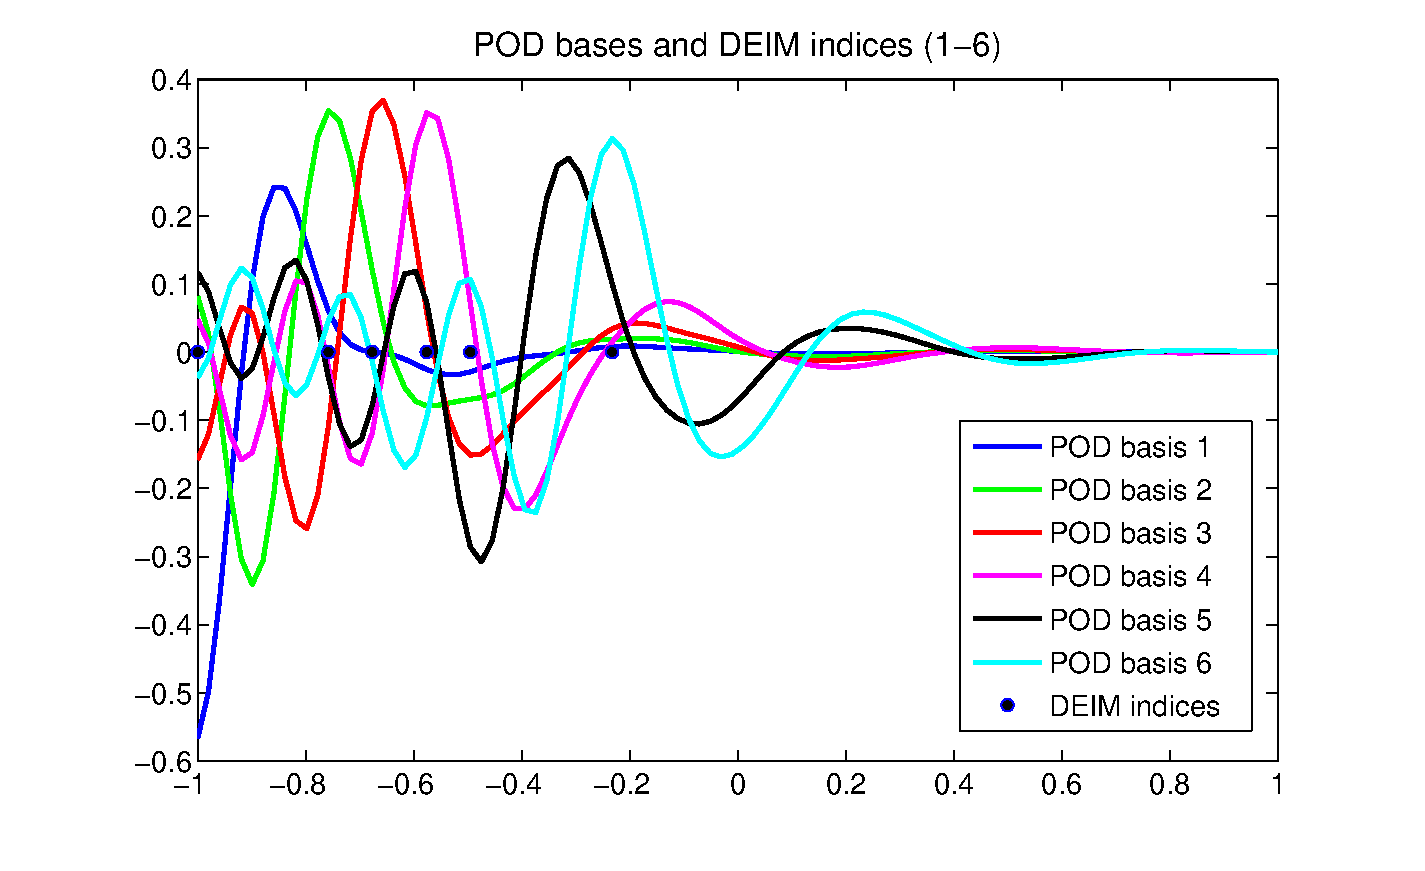
\includegraphics[width=0.49\textwidth]{plots/DeimPoints}}\hfill
\subfloat[DEIM approximation of dimension $10$.]{\label{DeimPointsb}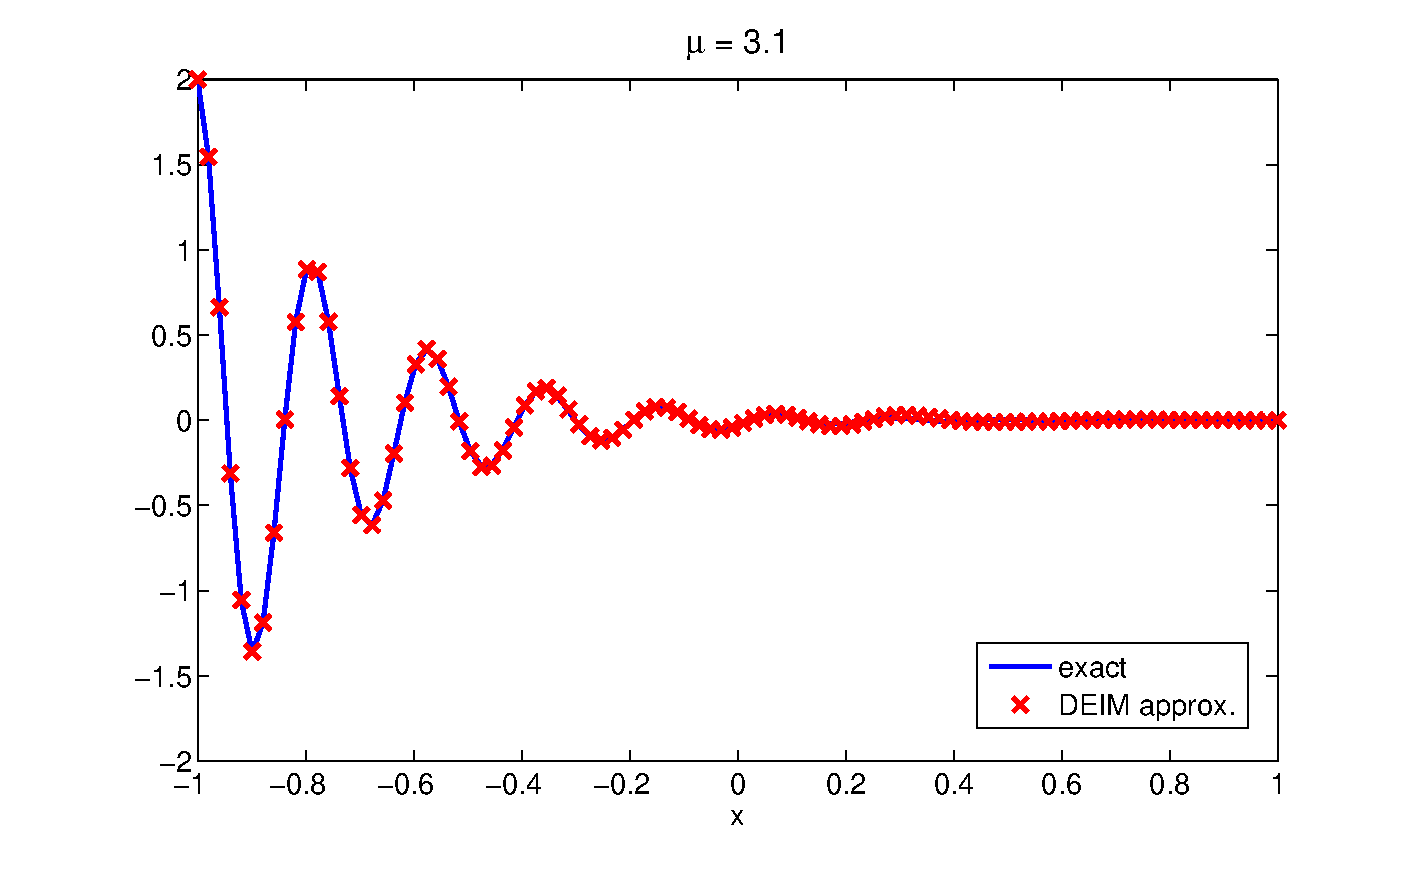
\includegraphics[width=0.49\textwidth]{plots/DeimApprox1D}}
\caption{The location of the DEIM indices for example \eqref{1Dex}.}\label{DeimPoints}
\end{figure}
%\subsubsection{Error bound for DEIM}
\begin{theorem}
\label{DEIMerrBound}
\emph{(Error bound of DEIM approximation, \cite{DEIM})}
\label{deimthm}
Let $\mathbf{f} \in \mathbb{R}^N$ be an arbitrary vector. Let $\{\mathbf{w}_i\}_{i=1}^m$ be the first $m$ left singular vectors of the snapshot matrix \eqref{snapshotF} (POD basis). From \eqref{approxF}, the DEIM approximation of order $m$ for $\mathbf{f}$ in the space $span \{\mathbf{u}_1,...,\mathbf{u}_m\}$ is
\begin{align*}
\mathbf{\hat f} = W(\mathcal{P}^T W)^{-1}\mathcal{P}^T \mathbf{f},
\end{align*}
where $W := [\mathbf{w}_1,...,\mathbf{w}_m] \in \mathbb{R}^{N \times m}$ and $\mathcal{P} := [\mathbf{e}_{\wp_1},...,\mathbf{e}_{\wp_m}] \in \mathbb{R}^{N \times m}$, with $\{\wp_1,...,\wp_m\}$ being obtained from Algorithm \ref{alg:DEIM} with input basis $\{\mathbf{w}_1,...,\mathbf{w}_m\}$. An error bound for $\mathbf{\hat f}$ is then given by
\begin{align*}
\|\mathbf{f} - \mathbf{\hat f}\|_2 \leq \mathcal{C} \cdot \mathcal{E}_*(\mathbf{f}),
\end{align*}
where
\begin{align*}
\mathcal{C} = \|(\mathcal{P}^T W)^{-1}\|_2, \quad \mathcal{E}_*(\mathbf{f}) = \|(I-W W^T)\mathbf{f}\|_2.
\end{align*}
The constant $\mathcal{C}$ is bounded by
\begin{align*}
\mathcal{C} \leq \frac{(1+\sqrt{2N})^{m-1}}{|\mathbf{e}^T_{\wp_1}\mathbf{w}_1|} = (1+\sqrt{2N})^{m-1} \|\mathbf{w}_1\|_\infty^{-1}.
\end{align*}
\end{theorem}
\begin{proof}
The proof is given in \cite[p. 2747-2749]{DEIM}.
\end{proof}
Not only does Theorem \ref{DEIMerrBound} give an error bound for the approximation obtained by the DEIM algorithm, but the proof also established that the choice of the DEIM indices in Algorithm \ref{alg:DEIM} in fact minimizes the growth of $\|(\mathcal{P}^T W)^{-1}\|_2$. Therefore, the algorithm is optimal in the sense that the approximation error is minimized.
\section{Application: POD-DEIM for the unsteady Burgers' equation}
\label{BurgersPODDEIM}
The following example is taken from \cite{KV99} where the authors applied POD to the one-dimensional Burgers' equation together with homogeneous Dirichlet boundary conditions and a step function $y_0(x)$ as initial condition has been considered,
\begin{equation}
\label{Burgers1}
\begin{split}
y_t + \left( \frac{1}{2}y^2 - \nu y_x\right)_x = f &, \quad (x,t) \in (0,L) \times (0,T), \\
y(t,0) = y(t,L) = 0&, \quad t \in (0,T), \\
y(0,x) = y_0(x)&, \quad x \in (0,L).
\end{split}
\end{equation}
Burgers' equation is a fundamental partial differential equation (PDE) from fluid dynamics and is, for instance, used in gas dynamics. The formulation \eqref{Burgers1} is known as the conservative form of Burgers' equation. Note that the numerical properties of \eqref{Burgers1} highly depend on the viscosity parameter $\nu$. For instance, when $\nu$ is small, the nonlinear term influences the numerical solution more and the PDE is called \textit{stiff}. This requires a small time step for the time integration.

For the numerical solution of the full-order system \eqref{Burgers1}, we used a finite element discretization in space using linear basis functions as described in  Appendix \ref{FEMDiscr_space}. This approach leads to the following system of ODEs:
\begin{align}
\label{FEMdiscr}
M \mathbf{\dot y}(t) = -\frac{1}{2} B \mathbf{y}^2(t) - \nu C \mathbf{y}(t) + \mathbf{f}
\end{align}
where $M$ is the mass matrix, $C$ is the stiffness matrix, and $B$ represents the convective term. For simplicity, we assume that the source term is zero, i.e. $f \equiv 0$. At this point, we also need to specify the initial condition $y_0(x)$:
\begin{align}
 \label{FEMdiscr_init}
 y_0(x) = \begin{cases} 1, & \text{ if } 0 \leq x \leq \frac{L}{2} \\ 0, & \text{ if } \frac{L}{2} < x \leq L \end{cases} \quad \Rightarrow \quad \mathbf{y}(0) = [1,...,1,0,...,0]^T \in \mathbb{R}^N.
\end{align}

The system \eqref{FEMdiscr} with initial condition \eqref{FEMdiscr_init} can be integrated in time using the implicit Euler method (see Appendix \ref{implEuler}). In Figure \ref{FullNumSol}, we present the numerical solution of \eqref{FEMdiscr}-\eqref{FEMdiscr_init} for different values of $\nu$ and $L = T = 1$.
\begin{figure}[H]
\centering
\subfloat{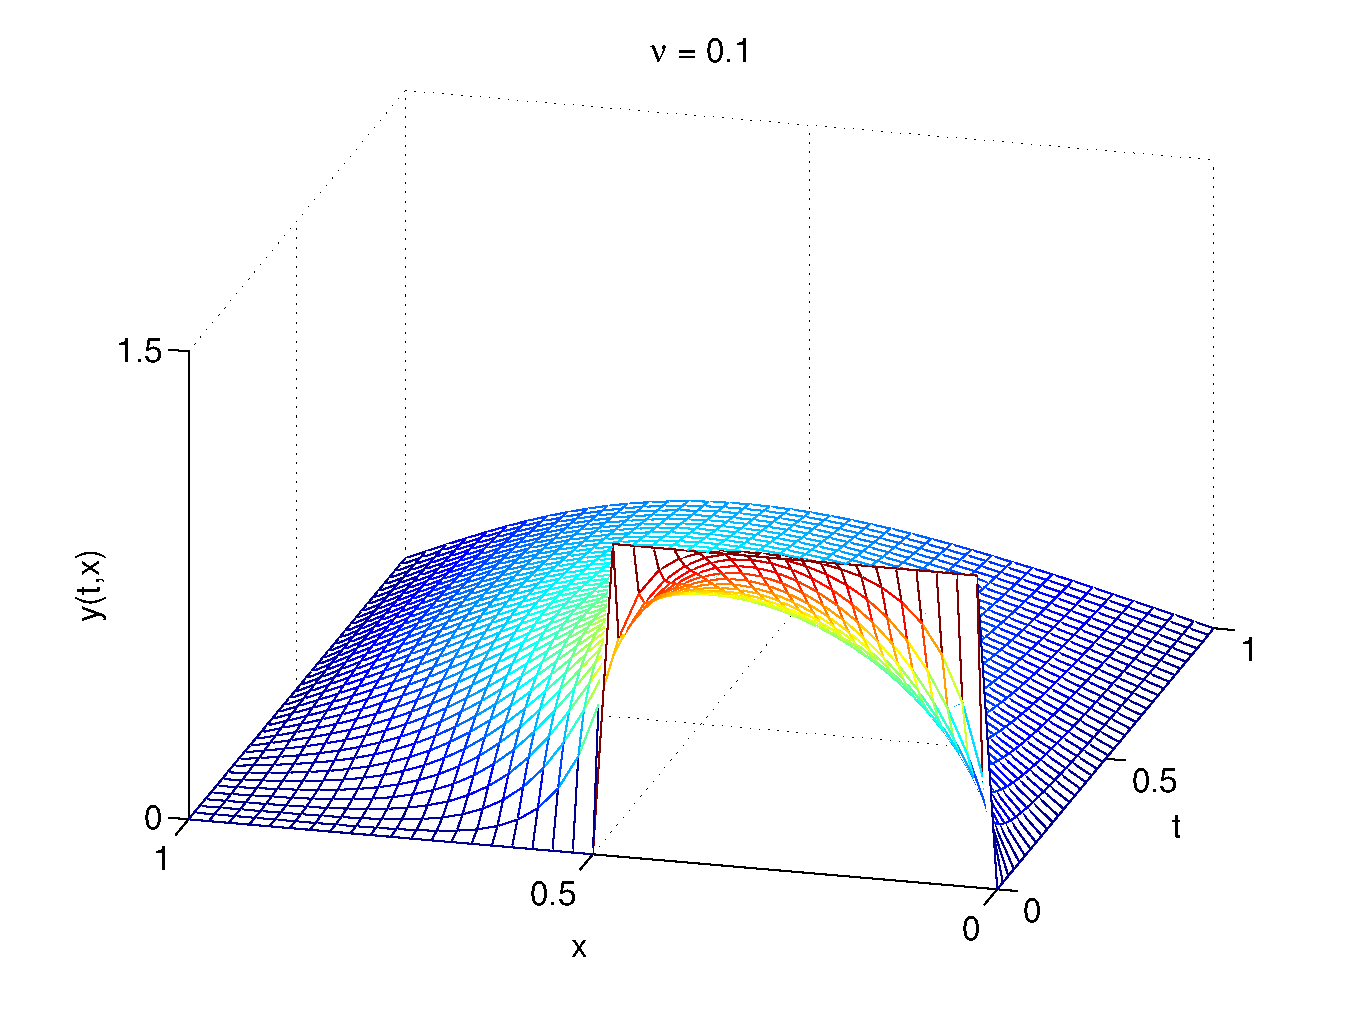
\includegraphics[width=0.33\textwidth]{plots/FullModel_nu01}}\hfill
\subfloat{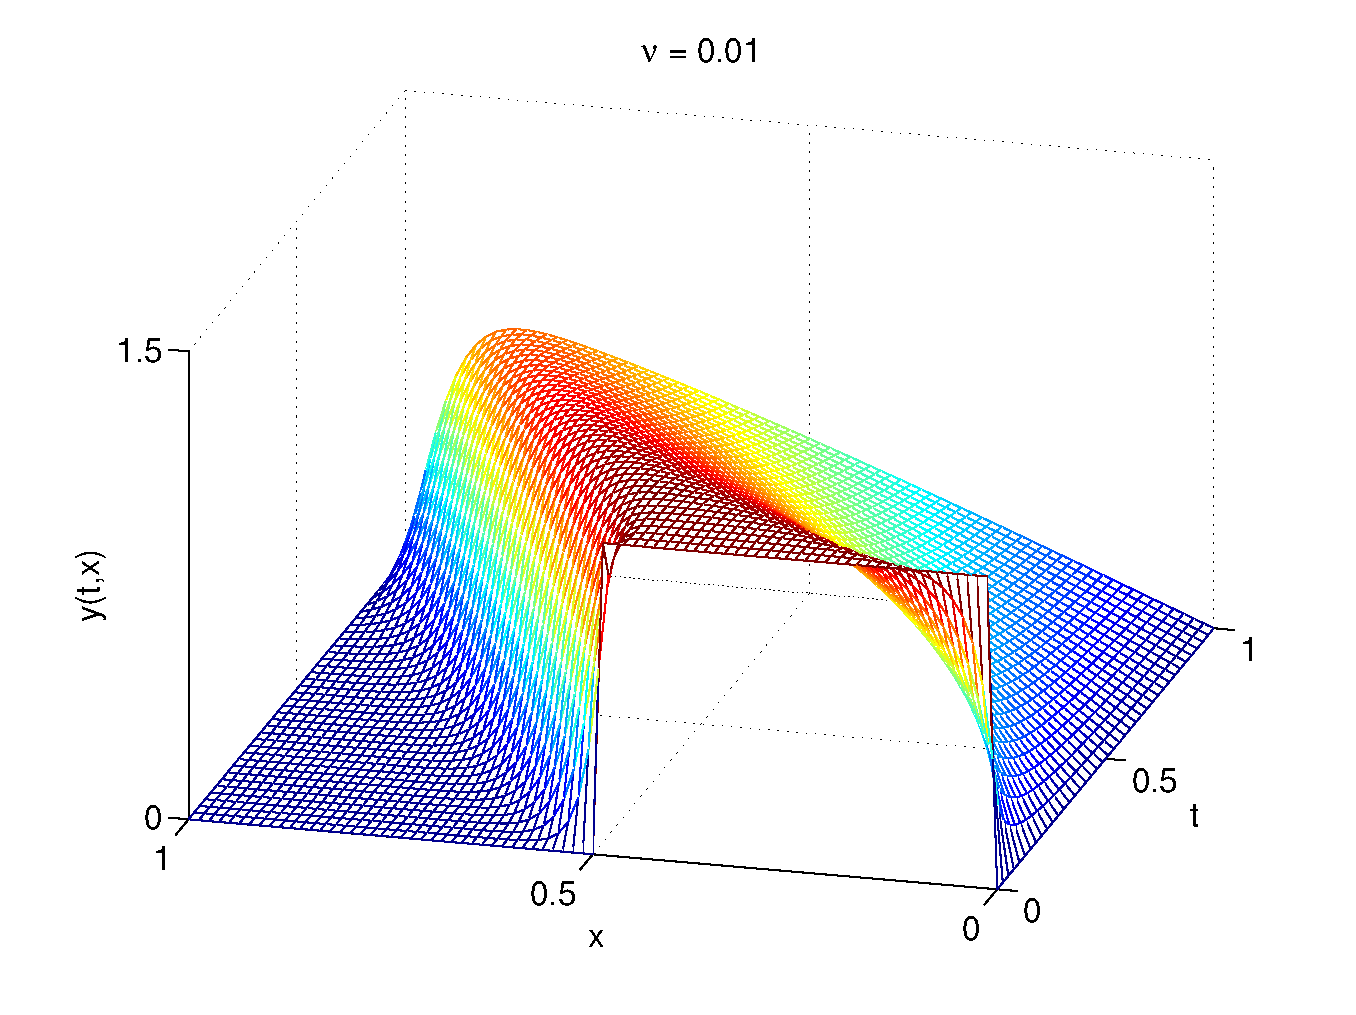
\includegraphics[width=0.33\textwidth]{plots/FullModel_nu001}}\hfill
\subfloat{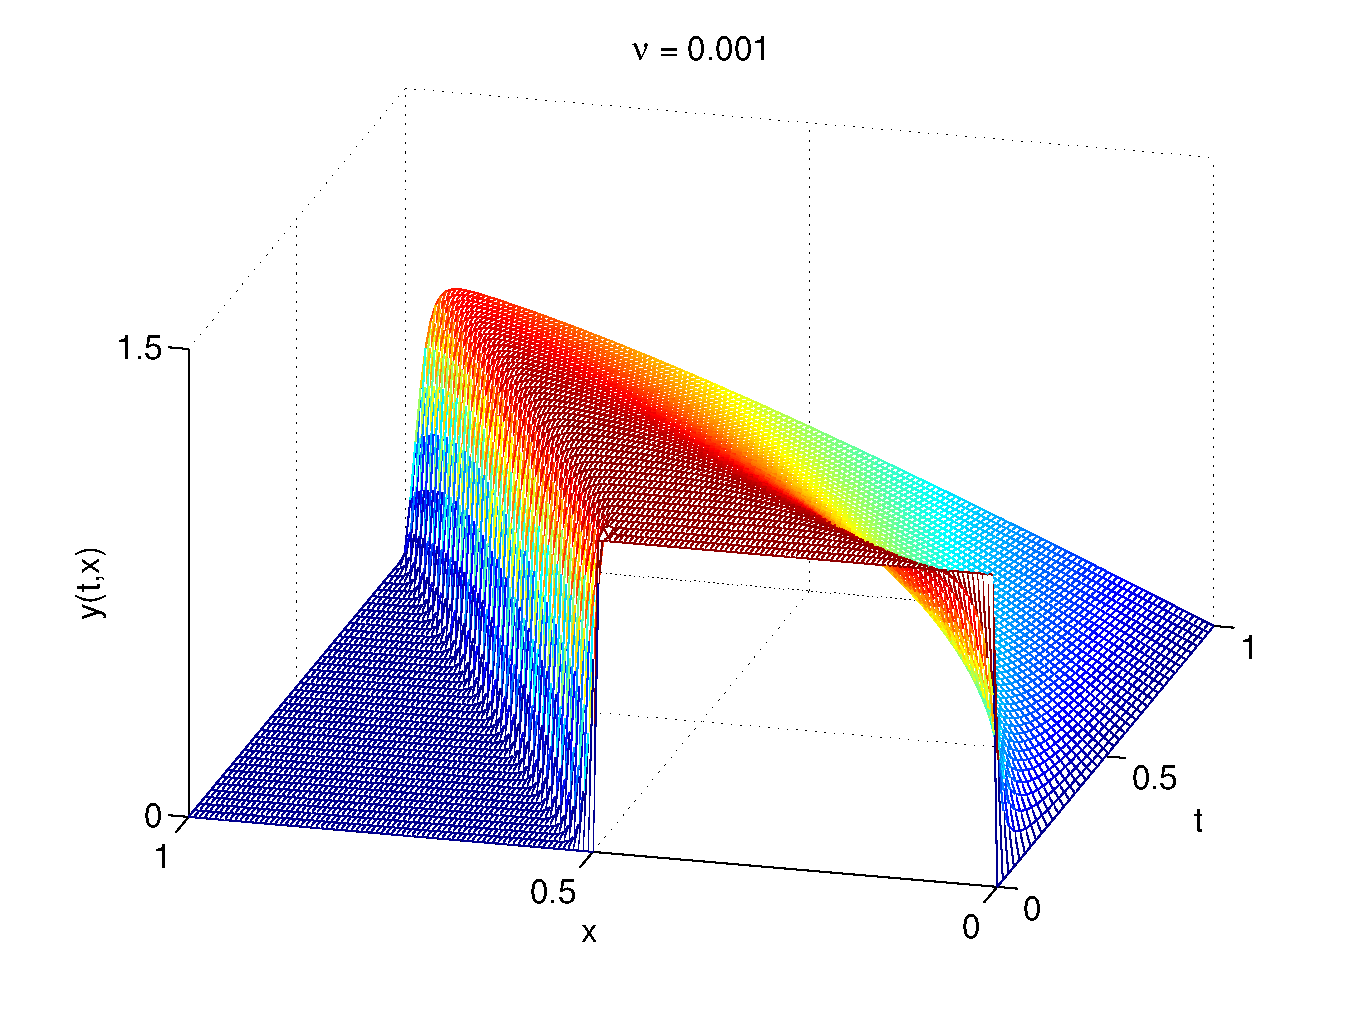
\includegraphics[width=0.33\textwidth]{plots/FullModel_nu0001}}\hfill
\caption{Numerical solution of the full-order Burgers' equation for different viscosity parameters $\nu = \{0.1, 0.01, 0.001\}$ and initial condition \eqref{FEMdiscr_init}.}\label{FullNumSol}
\end{figure}
According to \cite{KV99} the POD basis $\{\varphi_i\}_{i=1}^\ell$ can be obtained by solving the eigenvalue problem:
\begin{align}
\label{PODviaEW}
Y Y^T M \varphi = \sigma^2 \varphi,
\end{align}
where $Y$ is the matrix of snapshots as previously defined in \eqref{snapshots}, i.e. the columns of $Y$ are the solution of Burgers' equation at different time instances.

Since the mass matrix $M$ is symmetric and positive definite, there exists a Cholesky decomposition of the form $M = R^T R$. Multiplication of \eqref{PODviaEW} from the left with $R$ then yields,
\begin{align*}
R Y Y^T R^T R \varphi = \sigma^2 R \varphi,
\end{align*}
which is equal to
\begin{align}
\label{PODviaEW_final}
\bar{Y} \bar{Y}^T \bar{\varphi} = \sigma^2 \bar{\varphi},
\end{align}
for $\bar{Y} := RY$ and $\bar{\varphi} := R \varphi$. Because of the relation \eqref{SVDalsEW} between the SVD and eigenvalues, we can solve \eqref{PODviaEW_final} and, thus, also \eqref{PODviaEW} by the computation of an SVD of the matrix $\bar{Y} = RY$,
\begin{align}
\label{SVD_ss}
R Y = U \Sigma V^T.
\end{align}
After choosing a suitable POD dimension $\ell \ll N$, let us define the matrix of left singular vectors, $U_{\ell} := [u_1,...,u_{\ell}]$, where $u_i$ are the columns of the matrix $U$ in \eqref{SVD_ss}. Then, the POD basis is given by:
\begin{align}
\label{Phidef}
\Phi_{\ell} := R^{-1} U_{\ell},
\end{align}
and we denote the columns of $\Phi_\ell$ by $\varphi_i$ such that $\Phi_\ell = [\varphi_1,...,\varphi_\ell]$. The following ansatz leads to an approximation of the original full-order solution,
\begin{align}
\label{PODansatz}
\mathbf{y}(t) \approx \Phi_{\ell} \mathbf{\tilde y}(t) \quad \text{with } \mathbf{\tilde y}(t) \in \mathbb{R}^{\ell}.
\end{align}
The Galerkin projection of \eqref{FEMdiscr} onto $span \{\varphi_1,...,\varphi_\ell\}$ is given by
\begin{align}
\label{redSys}
\mathbf{\dot{\tilde y}}(t) = -\frac{1}{2} B_{\ell} (\Phi_{\ell} \mathbf{\tilde y}(t))^2 - \nu C_{\ell} \mathbf{\tilde y}(t),
\end{align}
with the matrices
\begin{align}
\label{Bl}
B_{\ell} &:= \Phi_{\ell}^T B \in \mathbb{R}^{\ell \times N},\\
\label{Cl}
C_{\ell} &:= \Phi_{\ell}^T C \Phi_{\ell} \in \mathbb{R}^{\ell \times \ell},
\end{align}
and with the new mass matrix equal to the $\ell \times \ell$ identity since:
\begin{align}
\label{Mortho}
M_{\ell} &:= \Phi_{\ell}^T M \Phi_{\ell} = U_{\ell}^T U_{\ell} = I_{\ell} \in \mathbb{R}^{\ell \times \ell}.
\end{align}
We will refer to \eqref{redSys} as the POD-reduced system. As shown in \eqref{Mortho}, due to the M-orthogonality of the projection matrix $\Phi_\ell$, the mass matrix in the POD-reduced system vanishes, and this leads to a simpler numerical treatment of \eqref{redSys} compared to the full-order system \eqref{FEMdiscr}. Note, that $\Phi_\ell \mathbf{\tilde y}(t) \in \mathbb{R}^N$ is still of large dimension and, therefore, no dimension reduction for the nonlinearity has been obtained so far. Also, the number of columns of the reduced matrix $B_\ell$ is still of large dimension $N$.

The projected initial condition for the original system is:
\begin{align*}
\Phi_{\ell} \mathbf{\tilde y}(0) &= \mathbf{y}(0), \\
R^{-1} U_{\ell} \mathbf{\tilde y}(0) &= \mathbf{y}(0),
\end{align*}
and, therefore, the initial condition for \eqref{redSys} can be obtained by pre-multiplication of the full-size initial condition with the matrix product $\Phi_{\ell}^T M$ as shown below:
\begin{align}
\label{initRed}
\mathbf{\tilde y}(0) &= U_{\ell}^T R \mathbf{y}(0) = \Phi_{\ell}^T R^T R \mathbf{y}(0) = \Phi_{\ell}^T M \mathbf{y}(0).
\end{align}
%Note that the initial condition of the full-order system is given in \eqref{FEMdiscr_init} and, thus, the respective initial condition of the reduced model follows directly from \eqref{initRed}.
%
As it has already been pointed out, the nonlinear term in \eqref{redSys} is still of large dimension $N$. We will now apply the DEIM method in order to reduce the computational complexity of evaluating the nonlinearity. Consider the snapshot matrix of the nonlinearity, \mbox{$F := [\mathbf{y}(t_1)^2,...,\mathbf{y}(t_{n_s})^2]$} and the corresponding Singular Value Decomposition:
\begin{align*}
 F = U_f \Sigma_f V_f^T.
\end{align*}
Again, by choosing the DEIM-dimension $m$, we are able to define the matrix of left singular vectors, $U_{m} := [u^f_1,...,u^f_{m}]^T$, which is used as an input basis for \mbox{Algorithm \ref{alg:DEIM}}. From \mbox{Algorithm \ref{alg:DEIM}}, we obtain the projection matrix $\mathcal{P}$ and the nonlinear term becomes:
\begin{align*}
 \Phi_{\ell}^T B (\Phi_{\ell} \mathbf{\tilde y})^2 = \Phi_{\ell}^T B U_{m} (\mathcal{P}^T U_{m})^{-1} \mathcal{P}^T (\Phi_{\ell} \mathbf{\tilde y})^2 \stackrel{(*)}{=} \underbrace{\Phi_{\ell}^T B U_{m} (\mathcal{P}^T U_{m})^{-1}}_{\ell \times m}(\underbrace{\mathcal{P}^T \Phi_{\ell}}_{m \times \ell} \mathbf{\tilde y})^2,
\end{align*}
where the step $(*)$ is allowed since squaring is a componentwise operation.
\newpage
\begin{figure}[H]
\centering
\subfloat{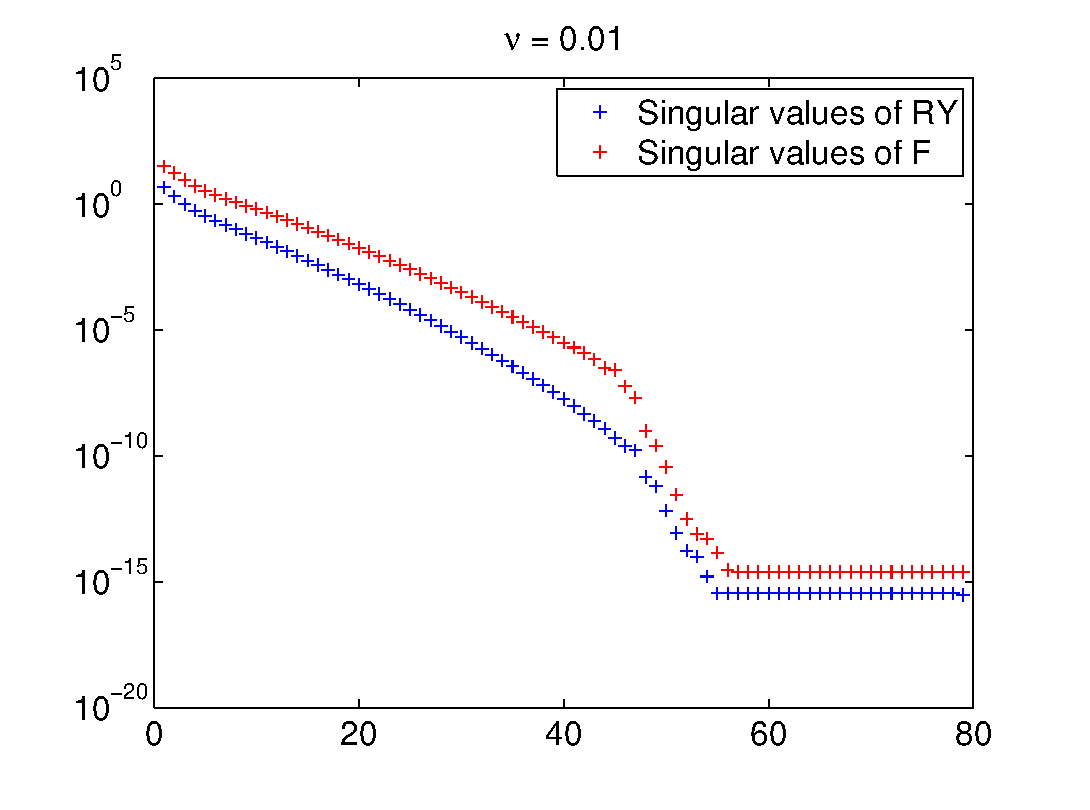
\includegraphics[width=0.49\textwidth]{plots/singValues_bignu}}\hfill
\subfloat{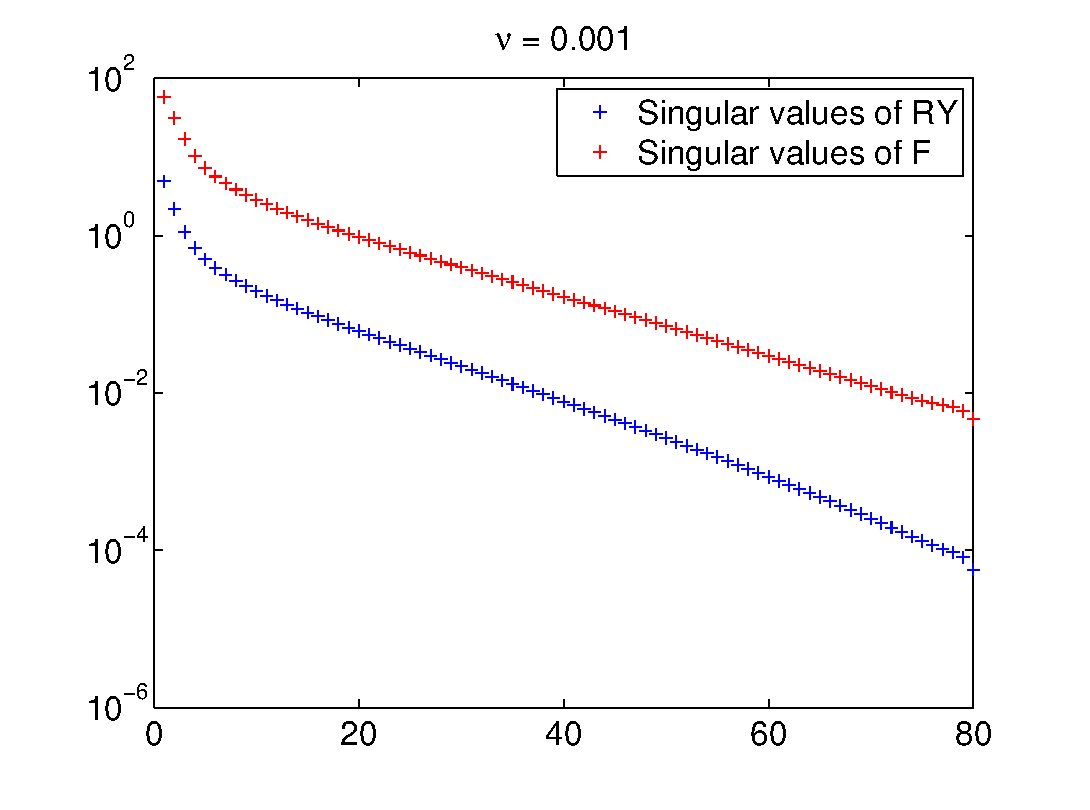
\includegraphics[width=0.49\textwidth]{plots/singValues_smallnu}}\hfill
\caption{Distribution of the singular values for $\nu = 0.01$ (left) and $\nu = 0.001$ (right).}\label{singVal}
\end{figure}
\noindent
The fully reduced POD-DEIM system is then given by
\begin{align}
\label{finalPODDEIM}
\mathbf{\dot{\tilde y}}(t) = -\frac{1}{2} \tilde B (\tilde F \mathbf{\tilde y}(t))^2 - \nu \tilde C \mathbf{\tilde y}(t) + \mathbf{\tilde f},
\end{align}
where
\begin{align}
\label{Bred}
\tilde{B} &:= \Phi_\ell^T B U_f(\mathcal{P}^T U_f)^{-1} \in \mathbb{R}^{\ell \times m},\\
\label{Cred}
\tilde{C} &:= \Phi_\ell^T C \Phi_\ell \in \mathbb{R}^{\ell \times \ell},\\
\label{Fred}
\tilde{F} &:= \mathcal{P}^T \Phi_\ell \in \mathbb{R}^{m \times \ell}.
\end{align}
Note that both matrices $\tilde{B}$ and $\tilde{F} $ can be pre-computed such that the system \eqref{finalPODDEIM} is indeed of dimension $\ell \times \ell$ and no dependence on the original \mbox{size $N$} exists anymore. As for the full-order system \eqref{FEMdiscr}, the POD-DEIM reduced system \eqref{finalPODDEIM} was solved by means of the implicit Euler method, see Appendix \ref{implEuler}. The choice of the dimensions of the reduced model $\ell$ and $m$ is crucial in order to obtain an accurate result of the reduced system that reproduces the dynamics of the original system. A good estimate for the choice of $\ell,m$ is given by the ration of the truncated sum of the singular values and the sum of all singular values given in \eqref{heuristics}. Therefore, we consider the distribution of the singular values of the respective snapshot matrices in Figure \ref{singVal}. We see that especially for $\nu = 0.01$, the first singular values decay tremendously which gives rise to a good approximation of the reduced system when only a small number for $\ell,m$ is chosen. We will present in Figure \ref{PODplot} the behavior of the numerical solution of the POD-DEIM reduced system when the DEIM-dimension $m$ is fixed and $\ell$ is increased.
\newpage
\begin{figure}[H]
  \centering
  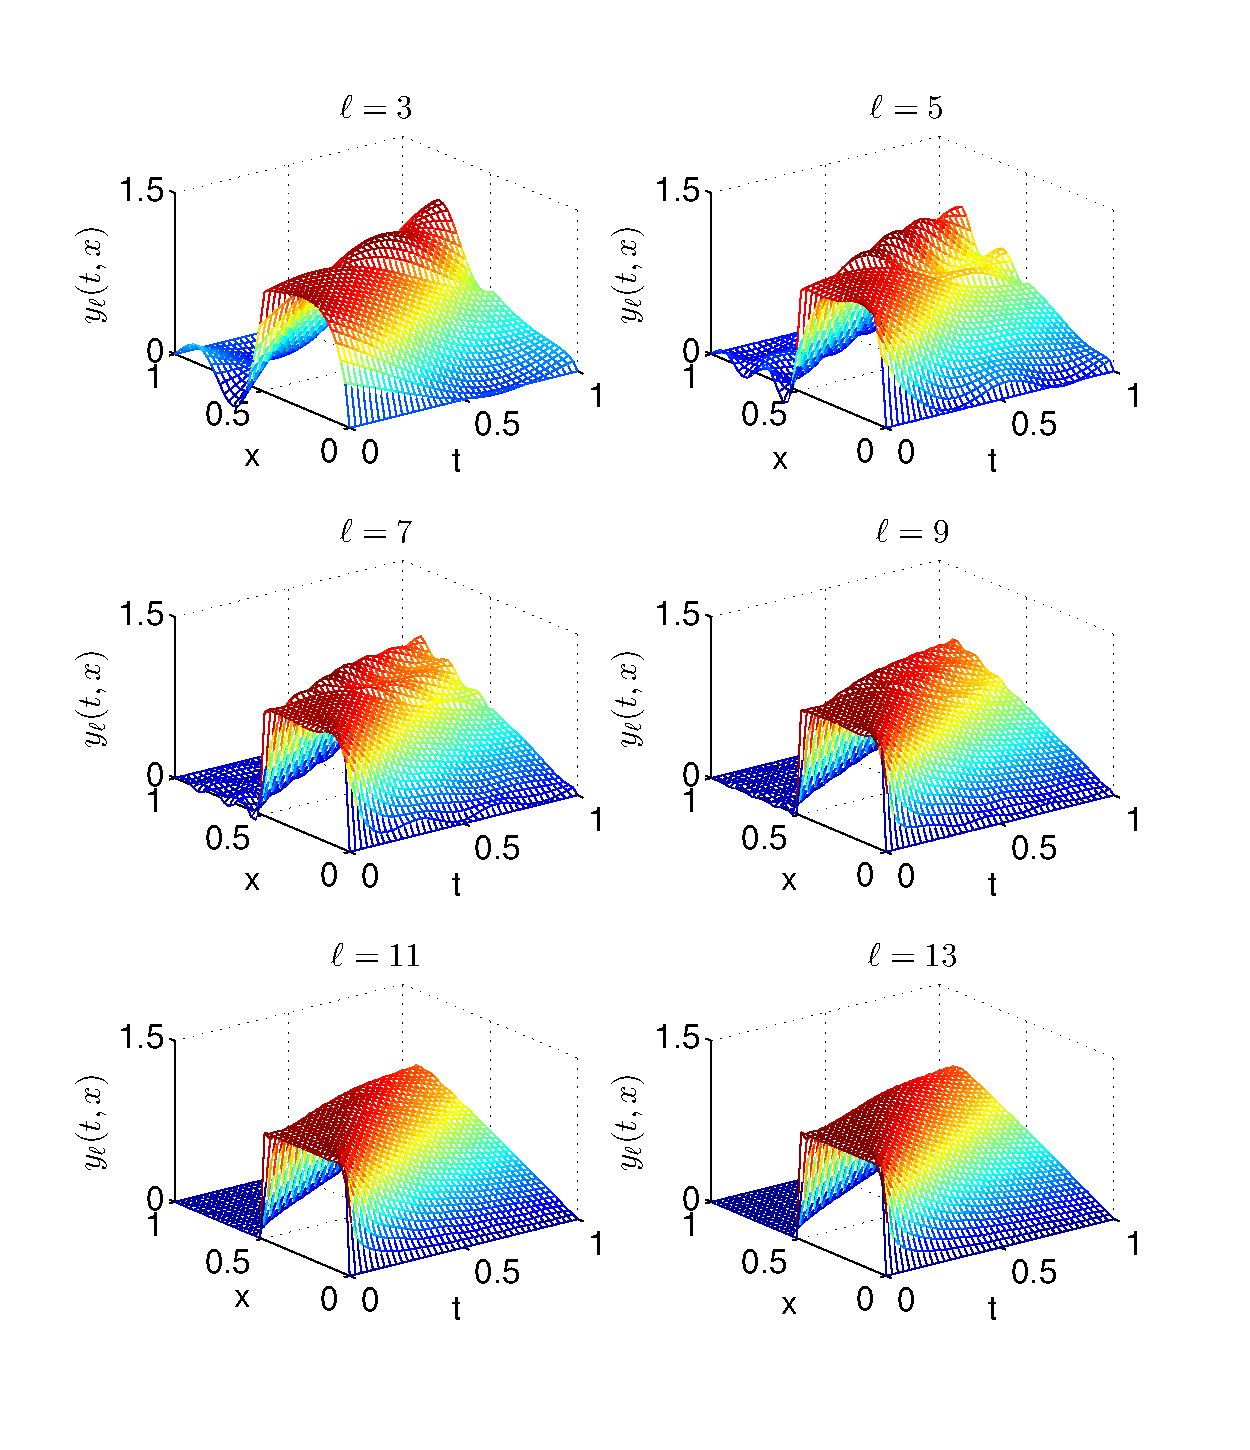
\includegraphics[width=\textwidth]{plots/PODplot_lnew.eps}\\
  \caption{POD-DEIM approximations for different dimensions $\ell$ and $m = 15$, $\nu = 0.01$.}\label{PODplot}
\end{figure}
Figure \ref{PODplot} shows the convergence of the POD-DEIM reduced model to the full-order solution. In each computation, a fixed DEIM dimension of $m = 15$ was used to approximate the nonlinear term in Burgers' equation. If the dimension of the POD basis $\ell$, i.e. the size of the projected model is increased, we see from Figure \ref{PODplot} that the numerical solution of the reduced system converges towards a smooth solution that corresponds to the solution of the original model.
\subsection{Approximation error}
We now focus on the accuracy of the approximated system's response computed with reduced models. Let $\mathbf{y}$ be the response of the full-order system, $\mathbf{y}^{(\ell)} = \Phi_\ell \mathbf{\tilde y}$ be the response of the POD-reduced model \eqref{redSys} obtained with a POD basis of dimension $\ell$, and let $\mathbf{y}^{(\ell,m)} = \Phi_\ell \mathbf{\tilde y}$ be the response of a reduced model obtained with POD-DEIM \eqref{finalPODDEIM}, with a POD basis is of dimension $\ell$ and a DEIM basis of dimension $m$. Then, we define the $L_2(\Omega)$ relative error in an approximate response $\mathbf{\bar{y}}$ with respect to the full-order-system's response $\mathbf{y}$ as:
\begin{align}
\label{relErr_def}
\bar{e} := \frac{\|\mathbf{y} - \mathbf{\bar{y}}\|_{L_2(\Omega)}}{\|\mathbf{y}\|_{L_2(\Omega)}} \approx \frac{\sqrt{h \cdot \delta \! t \cdot \sum_{i,j} [y_i(t_j) - \bar{y}_i(t_j)]^2}}{\sqrt{h \cdot \delta \! t \cdot \sum_{i,j} y_i^2(t_j)}},
\end{align}
where $\Omega = [0,L] \times [0,T]$, and $h$ and $\delta \! t$ are the step size in space and time, respectively. In our test cases, we have chosen $T = L = 1$ and, hence, $\Omega = [0,1] \times [0,1]$. The approximate response $\mathbf{\bar{y}}$ in \eqref{relErr_def} is  $\mathbf{\bar{y}} = \mathbf{y}^{(\ell)}$ for POD and $\mathbf{\bar{y}} = \mathbf{y}^{(\ell,m)}$ for POD-DEIM.

%In order to show the convergence of the reduced POD-DEIM model to the full-order system in more detail, we computed both, the numerical solution of the full-order system $\mathbf{y}$ as well as the numerical solution of the reduced-order model which we denote by $\mathbf{y}^{(\ell,m)}$. By the superscript we mean that $\mathbf{y}^{(\ell,m)}(t) = \Phi_\ell \mathbf{\tilde y}(t)$, where the reduced variable $\mathbf{\tilde y}$ has been obtained by the POD-DEIM reduced model \eqref{finalPODDEIM} with POD dimension $\ell$ and DEIM-dimension $m$, respectively. For $\Omega = [0,L] \times [0,T]$, with $L = T = 1$, we define the relative error $e_{\ell}$ using an approximation of the $L_2(\Omega)$ norm as:
%\begin{align}
%\label{relErr_def}
%e_{\ell,m} := \frac{\|\mathbf{y} - \mathbf{y}^{(\ell,m)}\|_{L_2(\Omega)}}{\|\mathbf{y}\|_{L_2(\Omega)}} \approx \frac{\sqrt{h \cdot \Delta t \cdot \sum_{i,j} [\mathbf{y}_i(t_j) - \mathbf{y}^{(\ell,m)}_i(t_j)]^2}}{\sqrt{h \cdot \Delta t \cdot \sum_{i,j} \mathbf{y}_i^2(t_j)}},
%\end{align}
%where $h$ and $\Delta t$ are the step size in space and time, respectively. In the same way, we denote by $e_\ell$ the relative error that compares the full-order solution with an approximation obtained by the POD-reduced system \eqref{redSys} with the POD dimension equal to $\ell$.
In Figure \ref{relErr}, show the behavior of the relative error when either the DEIM-dimension is fixed (left) or the POD dimension is fixed (right). From the numerical results that have been obtained for a viscosity parameter $\nu = 0.01$ and a full-order dimension of $N = 80$, we observe that the error of the POD and the POD-DEIM reduced model are of the same magnitude until the POD dimension exceeds the DEIM-dimension which has been fixed in the left plot to $m = 15$. When $\ell$ is larger than $m$ in the left plot, we observe that only the POD-reduced model is still improved while the error of the POD-DEIM reduced model seems to be dominated by the error caused by the DEIM approximation of size $m = 15$. %Figure \ref{relErr} shows the behavior of the relative error as the POD dimension $\ell$ increases. We see from the plot that from $\ell = 11$ on, the relative error is of the order $\mathcal{O}(10^{-4})$. Since the full-order system consists of $N=50$ grid points in space, we conclude that in this specify setup the reduced order model of approximately one fifth of the size of the original system already leads to results of a very good accuracy.
\begin{figure}[H]
  \centering
  \subfloat{\includegraphics[width=0.49\textwidth]{plots/rel_Err_newleft_NEW}}\hfill
  \subfloat{\includegraphics[width=0.49\textwidth]{plots/rel_Err_newright_NEW}}\hfill
  \caption{Relative error of the POD and POD-DEIM approximation for a fixed number of DEIM basis $m = 15$ (left) and a fixed number of POD basis $\ell = 15$ (right).}\label{relErr}
\end{figure}
The right plot in Figure \ref{relErr} shows the same behavior, i.e. an increase of the DEIM-dimension does not lead to a better approximation once it is larger than a given POD basis dimension. In Figure \ref{relErrml}, we observe this behavior for all combinations of $(\ell,m)$ in a range of \texttt{3:2:39}. These observations seem to indicate that for optimal dimension reduction using the POD-DEIM approach, we need to choose $\ell$ and $m$ in such a way that they are almost of the same size.
\begin{figure}[H]
  \centering
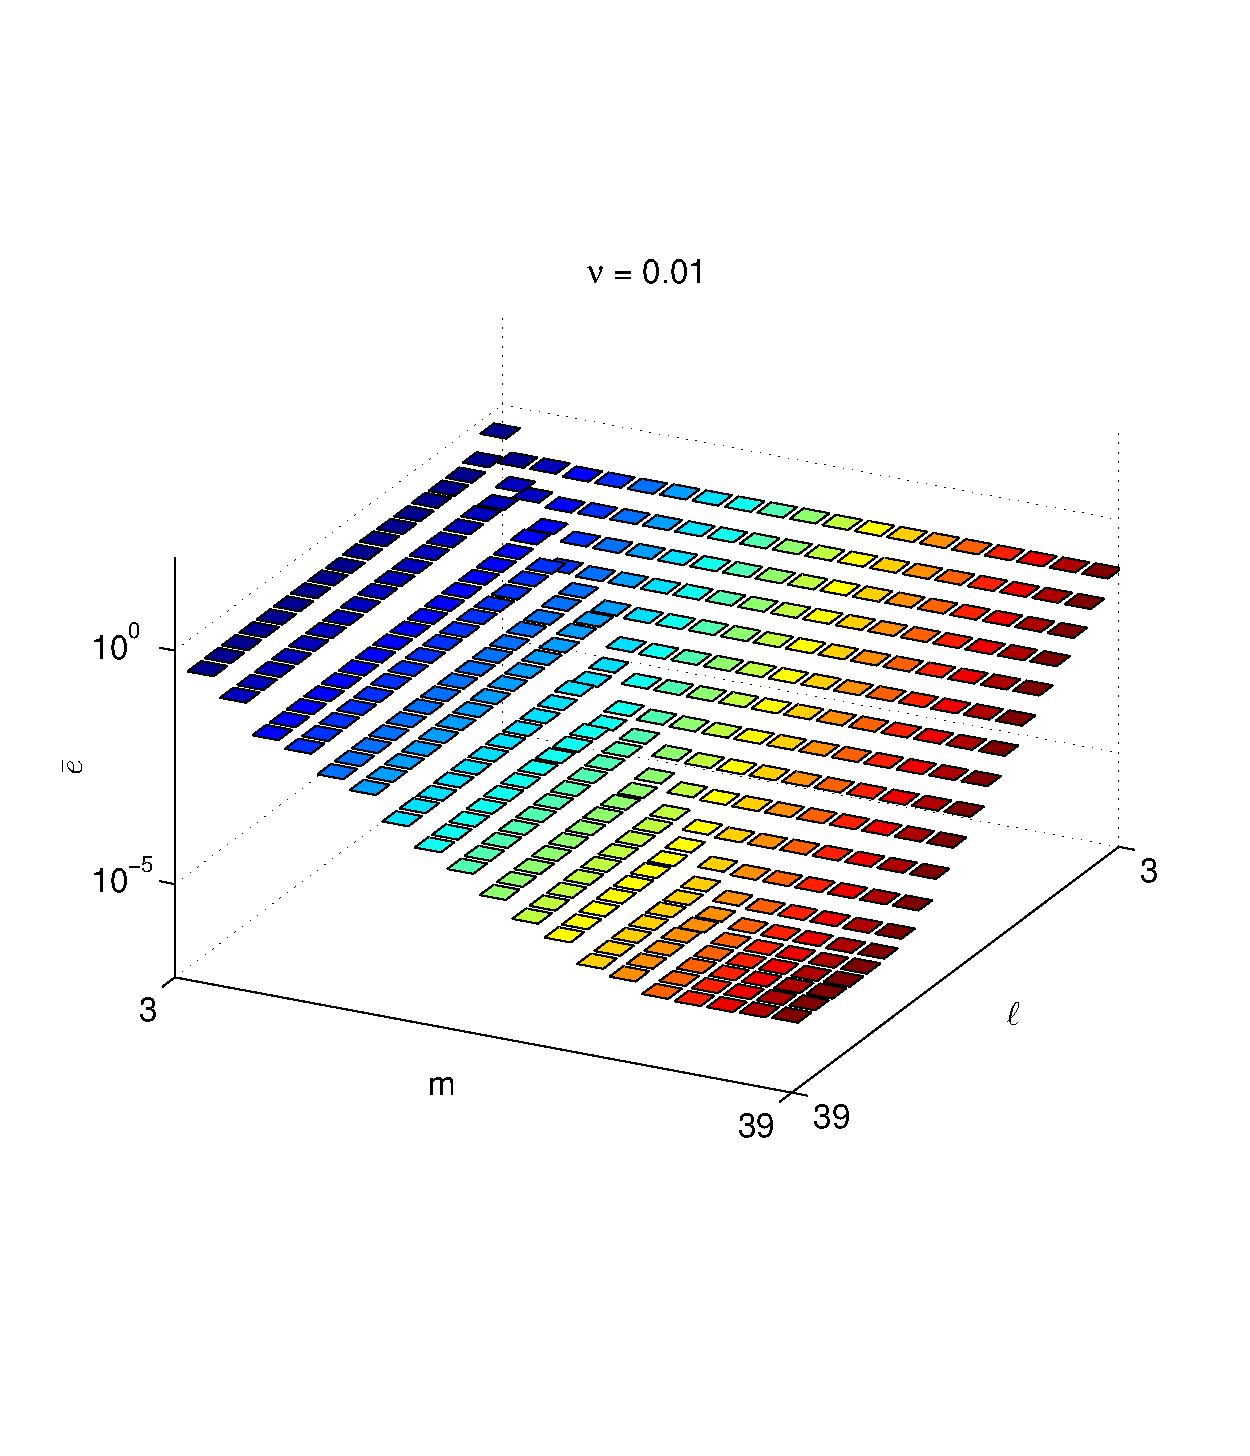
\includegraphics[width=0.7\textwidth]{plots/err_lm_NEW}
  \caption{Relative error of the POD-DEIM reduced model as a function of the reduced-model dimensions $\ell$ and $m$.}\label{relErrml}
\end{figure}

\subsection{Use of POD-DEIM for parameter studies}
In \cite{CS10}, the authors propose to use POD-DEIM also for parameter studies of a given dynamical system. In the case of Burgers' equation, this means that we simulate the full-order system twice for two different values of the viscosity parameters $\nu_{left} = 0.001$ and $\nu_{right} = 0.1$, using $N=400$ grid points in space which is necessary when dealing with very small values for $\nu$. The numerical solutions of the full-order system for both viscosity parameters were presented in Figure \ref{FullNumSol} where we can observe that the value of the viscosity parameter plays a crucial role in the propagation of the initial impulse in time. For large $\nu$, the solution becomes much more diffusive and, therefore, the initial condition vanishes very fast. For small $\nu$, the initial condition is propagated in time almost without losing height.
%\begin{figure}[H]
%\includegraphics[width=0.99\textwidth]{plots/param_study_both}
%\caption{Full-order system for $\nu=0.001$ (left) and $\nu = 0.1$ (right).}\label{param_study_both}
%\end{figure}
The benefit of POD-DEIM for parameter studies is that a reduced model can be obtained for any parameter $\nu$ that lies within the interval $[\nu_{left},\nu_{right}]$ only from data of the full-order model corresponding to $\nu_{left}$ and $\nu_{right}$. Suppose we are interested in an approximation of the numerical solution for $100$ different viscosity parameter in $[\nu_{left},\nu_{right}]$, we only need to solve the full-order system twice and are able to obtain a reduced model from these data.

The reduction is based on a singular value decomposition of the combined matrices
\begin{align*}
Y = [Y_{\ell} | Y_{r}], \quad F = [F_{\ell} | F_{r}],
\end{align*}
where $Y_{\ell}$ and $F_{\ell}$ are snapshot matrices of the solution and the nonlinearity corresponding to $\nu_{left}$ and $Y_{r}$ and $F_r$ correspond to $\nu_{right}$, respectively. The POD basis is then derived using the snapshot matrix $Y$ that contains information of the dynamical behavior of Burgers' equation with viscosity parameter $\nu_{left}$ and $\nu_{right}$. Similarly, the DEIM projection matrix $\mathcal{P}$ is obtained from the matrix $F$.

In Figure \ref{param_study_inner}, the POD-DEIM approximation for the viscosity parameter $\nu = 0.01$ using the dimensions $\ell = m = 45$ is presented as well as the full-order model of dimension $N = 400$ for the same viscosity parameter. The plot shows the good quality of the reduced system. At this point, we want to stress that in order to obtain the POD-DEIM model in Figure \ref{param_study_inner}, the simulation of the full-order system with parameter $\nu = 0.01$  was not taken into account. Therefore, the derivation of a reduced model for any parameter $\nu \in [\nu_{left}, \nu_{right}]$ only requires the computational work of the numerical solution of the reduced system once the matrices $Y$ and $F$ are obtained.
\begin{figure}[H]
\includegraphics[width=0.99\textwidth]{plots/param_study_inner}
\caption{Response of the full-order system and of the POD-DEIM reduced model for $\nu=0.01$.}\label{param_study_inner}
\end{figure}
\subsection{Computational speedup for POD and POD-DEIM}
\label{sect2_numTests}
In the previous chapters, the main focus lies on the size of the reduced system and the quality of the approximation compared to the full-order system. In this section, we are interested in the speedup of the computation when POD or POD-DEIM is applied. Therefore, we consider the numerical solution of Burgers' equation as described in Appendix \ref{FEMDiscr} for different viscosity parameters $\nu$. From the numerical analysis of the full model, it is well-known that for different sizes of $\nu$ a different size of the spatial discretization is required in order to obtain a stable numerical solution. In \ref{Tab2}, we have chosen the smallest value of $N$ for which the full-order solution is stable.

The following quantities have been measured during the numerical simulation:
\begin{itemize}
  \item $t_{setup}$ - The time which is required to pre-compute the matrices \eqref{Bl}, \eqref{Cl} in the case of pure POD and \eqref{Bred}-\eqref{Fred} in the case of POD-DEIM. Note that this only has to be performed once.
  \item $t_{PDEsol}$  - The time for the numerical solution of Burgers' equation. This has been done via the implicit Euler method and a Newton iteration for the time integration and a finite elements approach for the spatial discretization.
  \item $\bar{e}[10^{-4}]$  - The relative error in $L_2([0,1] \times [0,1])$ as defined in \eqref{relErr_def}.
  \item $S_P^{(1)}$  - The overall speedup which is defined as the ratio of the computational time for the full-order model and the respective reduced model.
  \item $S_P^{(2)}$ - The speedup when only the numerical solution of Burgers' equation is taken into account. Here, we neglect the time that is required for the pre-computation in $t_{setup}$.
\end{itemize}

In order to obtain comparable results, we decided to choose the reduced dimensions $\ell$ and $m$ such that the relative error $\bar{e}$ in the response of each of the reduced models has the same order of magnitude, $\bar{e} \in \mathcal{O}(10^{-4})$. Therefore, we indicate in the first row of \mbox{Table \ref{Tab2}} the important dimension from the respective model. In case of the full-order model, we present the number $N$ of ansatz function of the FEM discretization. For the pure POD reduced model we give the size of the POD basis, $\ell$, and for the the POD-DEIM reduced model we present the dimensions as a tuple $(\ell,m)$.
\begin{table}[H]
\centering
\begin{tabular}{|c|c|c|c|c|c|c|c|c|c|}
\cline{1-10}
 & \multicolumn{3}{ c| }{$\nu = 0.01$} & \multicolumn{3}{ c| }{$\nu = 0.001$}& \multicolumn{3}{ c| }{$\nu = 0.0001$}\\ \cline{2-10}
 & Full & POD & DEIM & Full & POD & DEIM & Full & POD & DEIM \\ \cline{1-10}
$N$/$\ell$/$m$ & $80$ &$ 11 $&$(11,13)$ & $200$&$35 $& $(35,40)$  & $800$&$40 $& $(40,55)$ \\ \cline{1-10}
$t_{setup}[s]$        & -      &0.003      &0.011       & -    &0.009&0.021 & -& 0.0729&0.182\\ \cline{1-10}
$t_{PDEsol}[s]$   &  0.068     &0.047      &0.040       & 0.232&0.12&0.055 & 4.416&0.276&0.085\\ \cline{1-10}
$\bar{e}[10^{-4}]$   & -      &6.13       &6.46        & -    &6.12&6.85 & -&7.43& 7.66\\ \cline{1-10}
$S_P^{(1)}$           & -      &1.35       &1.34        & -    &1.74&3.03 & -&12.54&16.52\\ \cline{1-10}
$S_P^{(2)}$           & -      &1.44       &1.71        & -    &1.88&4.21 & -&15.85&51.85\\ \cline{1-10}
\end{tabular}
\caption{Comparison between POD and POD-DEIM for different values of $\nu$.} \label{Tab2}
\end{table}
We first note that for all different sizes of the viscosity parameter $\nu \in \{0.01, 0.001, 0.0001\}$ it is in general possible to derive a POD and POD-DEIM reduced model of a tremendously smaller dimension and a high accuracy of $\bar{e} \in \mathcal{O}(10^{-4})$. The numerical tests of Table \ref{Tab2} are presented in order to illustrate two features of the POD-DEIM approach. Firstly, we see that the time which is required for the numerical solution of the POD-DEIM reduced model does not increase when the size of the original problem, $N$, increases. On the other hand, we see that the solution of the pure POD model still depends on the original problem size and increases with $N$. This behavior is illustrated in Figure \ref{depN} where we see that the increase in $N$ only affects the computation time of the POD model. Its independence of the original (large) dimension is the reason for the large speedup obtained when using the POD-DEIM reduced model. We see that for $N=3,000$, the POD-DEIM model is almost five times faster than the pure POD model. Secondly, we observe that in order to apply DEIM, it is more costly to apply the required pre-computations of the matrices \eqref{Bred}-\eqref{Fred}. This is mostly because two singular value decompositions are required in order to obtain the projection basis and the input basis for the DEIM Algorithm \ref{alg:DEIM}. This is also the reason why the overall speedup $S_P^{(1)}$ of POD and POD-DEIM for the presented test configurations is comparable even though DEIM leads to a higher speedup. The most important observation from the results in Table \ref{Tab2} is, however, that for the case $\nu = 0.0001$ and $N = 800$, we are able to show a speedup of the POD-DEIM method of more than $50$ compared to the full model while POD only leads to a speedup of $\sim \! 16$. This speedup computation only takes into account the time that is required to actually solve the reduced system numerically. Therefore, we conclude that DEIM leads to a tremendous reduction in computational cost as long as we are able to pre-compute the matrices \eqref{Bred}-\eqref{Fred} only once and then solve the reduced system many times. This conclusion gives rise to the application of POD-DEIM within an optimization iteration as described in the Chapter \ref{Opt_chap}.
\begin{figure}[H]
\centering
\subfloat{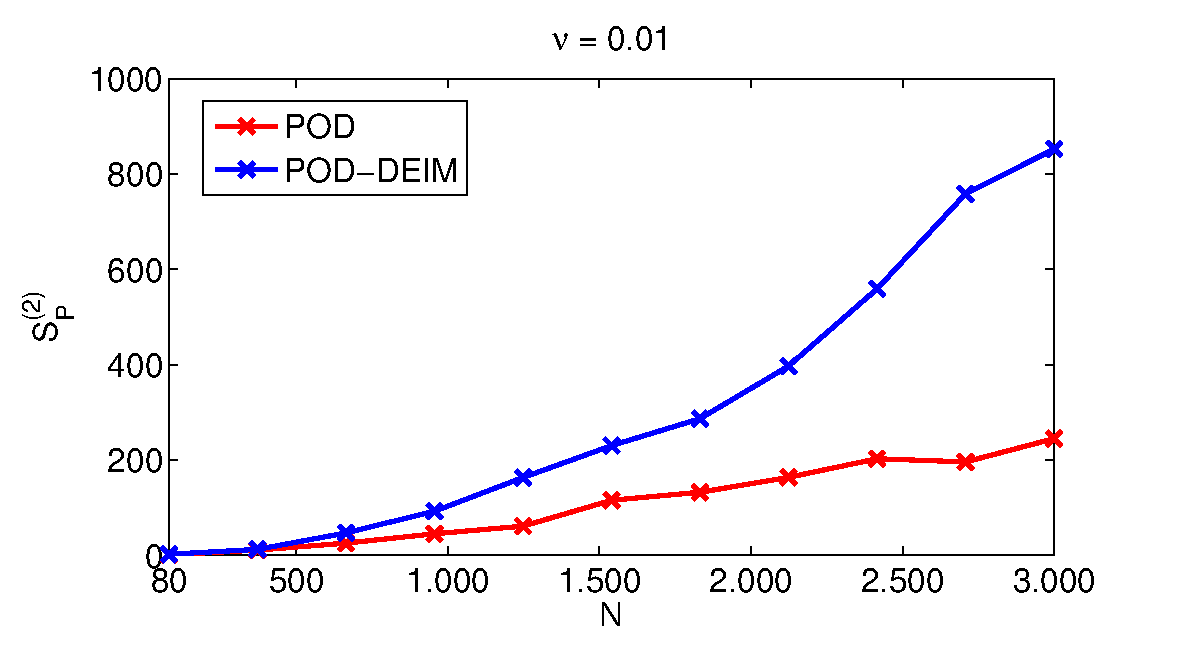
\includegraphics[width=0.49\textwidth]{plots/PODDEIM_Sp2}}\hfill
\subfloat{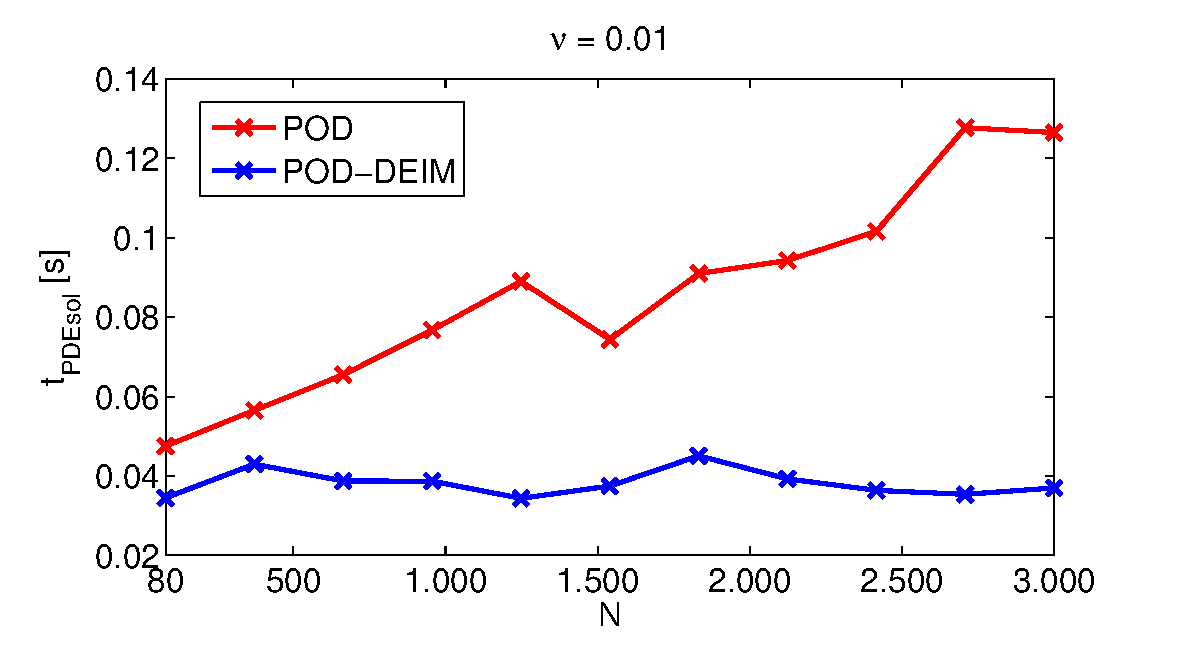
\includegraphics[width=0.49\textwidth]{plots/PODDEIM_Tsol}}\hfill
\caption{Dependence of the reduced models on the full-order dimension $N$.}\label{depN}
\end{figure}

%In the previous chapters, the main focus lies on the size of the reduced system and the quality of the approximation compared to the full-order system. In this section, we are interested in the speed-up of the computation when POD and POD-DEIM is applied. Therefore, we consider Burger's equation with viscosity parameter $\nu = 0.003$ on a spatial domain $[0,1]$ and end time $T = 4$. This requires a spatial and time discretization of $N = N_t =400$ points in order to obtain a stable numerical simulation. The reduced model with dimensions $\ell=m=45$ leads to an approximation of high accuracy (see Table \ref{Tab1}).
%
%The following quantities have been measured during the numerical simulation:
%\begin{itemize}
%  \item $t_s$ - The time which is required to pre-compute the matrices \eqref{Bl}, \eqref{Cl} in the case of pure POD and \eqref{Cl}, \eqref{Bred}, \eqref{Fred} in the case of POD-DEIM.
%  \item $t_{Eul}$ - The time for the time integration via the implicit Euler method and Newton's iteration.
%  \item $\bar e$ - The relative error in $L_2([0,1] \times [0,4])$.
%  \item $S_P$ - The overall speed-up which is defined as the ratio of the computational time for the full-order model and the reduced model.
%\end{itemize}
%In Table \ref{Tab1}, the speed-up of pure POD and POD-DEIM are compared: The application of POD of dimension $\ell = 45$ leads to a speed-up of the computation of approximately $3.5$ times the time of the original-size solution. If in addition DEIM is applied with dimension $m = 45$, we notice that the speed-up compared to the full-order model is $11.6$ which is approximately a speed-up of another $3.5$ times compared to the pure POD method. Therefore, in this setting the computational benefit of POD and POD-DEIM is almost of the same size. Note that both dimensions have been chosen in such a way that the relative error is of the order $\mathcal{O}(10^{-4})$ in both cases and, thus, the accuracy of the approximations is comparable for both cases.
%\begin{table}[H]
%\centering
%\begin{tabular}{l|c|c|c}
%& Full Order Model & POD & POD-DEIM \\
%\hline
%$t_s$ & - &  0.0018s& 0.0021s\\
%$t_{Eul}$ & 18.0785s& 5.1342s & 1.5189s\\
%$\bar e$ & - & 1.2805e-04 & 2.5057e-04\\
%$S_P$ & - &  3.5199 & 11.6801 \\
%\end{tabular}
%\caption{Comparison between POD and POD-DEIM for $\nu = 0.003$.} \label{Tab1}
%\end{table}

\chapter{Optimal control of partial differential equations}
\label{Opt_chap}
We consider the following optimization problem,
\begin{align}
\label{optControl}
\min_u \mathcal{J}(y(u),u),
\end{align}
where $y$ is the solution to a nonlinear, possibly time-dependent partial differential equation,
\begin{align}
\label{optControl_const}
c(y,u) = 0,
\end{align}
and $\mathcal{J}$ is called the \textit{cost function} or the \textit{objective function}. Since in order to evaluate \eqref{optControl} as a function of the control $u$ we first need to solve the constraining PDE \eqref{optControl_const}, the optimization problem \eqref{optControl}-\eqref{optControl_const} is referred to as an \textit{implicitly-constrained optimization problem} in \cite{H10}. Standard references for the numerical solution of optimization problems are in \cite{DS96,K99,NW06}. In general, one distinguishes between gradient-based and Newton-type methods which use information of the first and second derivative of the cost function, respectively.

An alternative way to look at \eqref{optControl}-\eqref{optControl_const} is to consider the following constrained optimization problem,
\begin{equation}
\label{allgControl}
\begin{split}
\min_u \ &\mathcal{J}(y,u) ,\\
\text{subject to } \ &c(y,u) = 0,
\end{split}
\end{equation}
where $y$ is called the \textit{state} and $u$ is considered to be the \textit{control} or the \textit{input} of the problem \eqref{allgControl}. Again, the scalar function $\mathcal{J}$ is usually called the \textit{cost function} and the \textit{constraint} $c$ is given by a nonlinear partial differential equation. Note, that $y \in \mathbb{R}^{n_y}$ and $u \in \mathbb{R}^{n_u}$ are typically high-dimensional and, therefore, the (given) functions $\mathcal{J}$ and $c$ map as follows,
\begin{align*}
\mathcal{J} : \mathbb{R}^{n_y} \times \mathbb{R}^{n_u} \rightarrow \mathbb{R}, \quad c : \mathbb{R}^{n_y} \times \mathbb{R}^{n_u} \rightarrow \mathbb{R}^{n_y}.
\end{align*}
%The usage of $n_y, n_u$ for the dimensions of the state and the control variable have been distinguished in order to keep \eqref{allgControl} in the most general form. Note that in the latter application, we will use $n_y = n_u = N$.
As it is stated in \eqref{allgControl}, we seek for an optimal control $u^* = \argmin_{u} \ \mathcal{J}(y,u)$ that minimizes the cost function $\mathcal{J}$ and at the same time fulfills the PDE $c$. In more detail, the control $u$ will appear on the right-hand side of the constraining partial differential equation $c$ such that the solution $y$ will depend on $u$. We will therefore sometimes write $y(u)$ in order to indicate that the solution to the PDE is only unique after $u$ is specified. Reference for optimal control of partial differential equations are \cite{B75,L71,T10}.
\section{Newton-type methods using adjoint techniques for derivative computation}
\label{optAdj}
For an easier notation, let us introduce the objective function as a function of the control only,
\begin{align}
\label{easyJ}
\hat{\mathcal{J}}(u) := \mathcal{J}(y(u),u).
\end{align}
The unconstrained optimization problem \eqref{optControl} then becomes,
\begin{align}
\label{minhatJ}
\min_u \hat{\mathcal{J}}(u),
\end{align}
where $\hat{\mathcal{J}} : \mathbb{R}^{n_u} \rightarrow \mathbb{R}$. Many textbooks on optimization deal with the numerical solution of \eqref{minhatJ}, cf. \cite{DS96,K99,NW06,Rao09}.

A standard approach to solve the optimization problem \eqref{minhatJ} is by solving iteratively the so-called Newton equation
\begin{align}
\label{Newtoneqn_J}
\nabla^2 \hat{\mathcal{J}}(u_k) s_k = -\nabla \hat{\mathcal{J}}(u_k),
\end{align}
where an initial control $u_0$ has to be chosen and in an outermost loop on $k$ one tries to reach convergence. In \eqref{Newtoneqn_J}, $s_k$ is the \textit{search direction} and $\nabla \hat{\mathcal{J}}$ and $\nabla^2 \hat{\mathcal{J}}$ are the gradient and the Hessian of the objective function, respectively. Note that \eqref{Newtoneqn_J} is a system of linear equations in the unknown search direction $s_k$. The new control is computed as:
\begin{align}
\label{update_u}
u_{k+1} = u_k + \alpha^*_k \cdot s_k,
\end{align}
where the optimal step size $\alpha^*_k \in \mathbb{R}_+$ has to be determined such that:
\begin{align}
\label{gen_line}
\alpha^*_k = \argmin_{\alpha_k \in \mathbb{R}_+} \mathcal{J}(y(u_k + \alpha_k \cdot s_k), u_k + \alpha_k \cdot s_k).
\end{align}
In practice, problem \eqref{gen_line} is solved approximately using a selected criterion. The optimization method in Algorithm \ref{alg:Opt} is a truncated-CG Newton method from \cite{H08}. In Algorithm \ref{alg:Opt}, an Armijo line search strategy  (see Appendix \ref{Armapp}) is used for approximately solving \eqref{gen_line} and a truncated Conjugate Gradient (CG) method is used for solving the Newton equation \eqref{Newtoneqn_J}, see Appendix \ref{CGapp}. The gradient and Hessian of the objective function are computed efficiently by means of the adjoint technique as described in Section \ref{adj_grad} and \ref{Hessadj}, respectively.
%Note that in order to evaluate the objective function $\mathcal{J}$ we need to compute the corresponding state $y$ which in our setting requires to solve the constraining PDE $c$. In Appendix \ref{Armapp} we present the Armijo line-search algorithm in order to solve \eqref{gen_line}, as it has been proposed in \cite{H08}. The optimization algorithm presented in this section will solve the Newton equation \eqref{Newtoneqn_J} by a truncated version of the conjugate gradient (CG) method, see Appendix \ref{CGapp}.  We will present how the gradient and the Hessian of the cost function  $\hat{\mathcal{J}}$ can be computed efficiently by so-called adjoint equations. An overview of the described optimization loop is presented in Algorithm \ref{alg:Opt}. The stopping criterion is given by a numerical check of the zero-gradient condition in line $6$.
\begin{algorithm}[H]
\caption{Truncated Newton-CG method with Armijo line search, \cite{H08}}
\label{alg:Opt}
\begin{algorithmic}[1]
\STATE Set initial control $u_0 = 0$, stopping tolerances $\varepsilon_\mathcal{J},\varepsilon_\nabla > 0$, \texttt{max\_newtoncg} $\in \mathbb{N}$
\FOR{$k = 0$ to \texttt{max\_newtoncg}}
\STATE Solve $c(y_k,u_k) = 0$ for $y_k$
\STATE Save $\mathcal{J}_{old} := \mathcal{J}(y_k,u_k)$
\STATE Compute $\nabla \hat{\mathcal{J}}(u_k)$ via algorithm \ref{alg:Adj1}
\IF{$\|\nabla \hat{\mathcal{J}}(u_k)\| < \varepsilon_\nabla$}
\RETURN
\ENDIF
%\STATE Compute $\nabla^2 \hat{\mathcal{J}}(u_k)$ via algorithm \ref{alg:Adj2}
\STATE Solve the Newton equation $\nabla^2 \hat{\mathcal{J}}(u_k) s_k = -\nabla \hat{\mathcal{J}}(u_k)$ via the truncated conjugate gradient method, see Appendix \ref{CGapp}, and using Algorithm \ref{alg:Adj2} to compute matrix-vector products with $\nabla^2 \hat{\mathcal{J}}(u_k)$
\STATE Obtain $\alpha_k^* \approx \argmin_{\alpha_k \in \mathbb{R}_+} \mathcal{J}(y(u_k + \alpha_k s_k),u_k + \alpha s_k)$ via the Armijo line search algorithm, see \mbox{Appendix \ref{Armapp}}
\STATE Update $u_{k+1} = u_k + \alpha_k^* s_k$
\IF{$|\mathcal{J}_{old} - \mathcal{J}(y(u_{k+1}),u_{k+1})| < \varepsilon_\mathcal{J}$}
\RETURN
\ENDIF
\ENDFOR
\end{algorithmic}
\end{algorithm}
Note that in Algorithm \ref{alg:Opt}, we have used two so-called numerical stopping criteria. The tolerance $\varepsilon_\nabla$ in line $6$ determines when the gradient of the objective function is almost zero which is a necessary condition to find a minimum. In line $12$, the tolerance $\varepsilon_\mathcal{J}$ checks if the change of the value of the objective function during the optimization iteration is sufficiently small.
\subsection{Using adjoint equations for gradient computation}
\label{adj_grad}
In order to derive an efficient numerical method to compute the gradient of $\hat{\mathcal{J}}$ as proposed in \cite{H08}, let us introduce the Lagrangian function $\mathcal{L}$ which converts the constrained optimization problem \eqref{allgControl} into an unconstrained optimization problem. The Lagrangian function is defined via
\begin{align}
\label{genLagr}
&\mathcal{L} : \mathbb{R}^{n_y} \times \mathbb{R}^{n_u}  \times \mathbb{R}^{n_y} \rightarrow \mathbb{R} \nonumber \\
&\mathcal{L}(y,u,\lambda)= \mathcal{J}(y,u) + \lambda^T c(y,u),
\end{align}
where $\lambda$ is a new variable called the \textit{Lagrange multiplier}. It is well-known that for all optimal points $(y^*,u^*)$ to the original constrained problem \eqref{allgControl}, there exists a $\lambda^*$ such that $(y^*,u^*, \lambda^*)$ is a stationary point of the Lagrangian function \eqref{genLagr}, cf. \cite{S86}. Stationary points of \eqref{genLagr} fulfill the first order optimality conditions (zero-gradient condition),
\begin{align}
\label{opt1}
\nabla_y \mathcal{L}(y,u,\lambda) &= 0,\\
\label{opt2}
\nabla_u \mathcal{L}(y,u,\lambda) &= 0,\\
\label{opt3}
\nabla_\lambda \mathcal{L}(y,u,\lambda) &= 0,
\end{align}
where the subscripts are used to denote partial derivatives with respect to the indicated variable. Note, that from \eqref{opt3} the original constraint $c(y,u) = 0$ follows directly. Furthermore, we will use \eqref{opt1} in order to derive the so-called \textit{adjoint equation} which determines the auxiliary variable $\lambda$. In the following, we will describe an efficient way to compute $\nabla \hat{\mathcal{J}}(u)$ which appears on the right-hand side of \eqref{genLagr} in Algorithm \ref{alg:Opt} based on the conditions \eqref{opt1}-\eqref{opt3}.
%In this section, we will describe an efficient way to obtain stationary points of the Lagrangian function \eqref{genLagr} numerically. Following \cite{H08}, we will use conditions \eqref{opt1} and \eqref{opt3} in order to derive efficient algorithms to solve condition \eqref{opt2} by the Newton equation. For simplicity of notation, we will introduce the function $\mathcal{\hat L}$ to be the Lagrangian as a function of the control $u$ only, i.e.
%\begin{align*}
%\mathcal{\hat L}(u) = \mathcal{L}(y,u,\lambda)\big|_{y=y(u), \lambda=\lambda(u)}.
%\end{align*}
%Consequently the corresponding gradient and Hessian can be denoted in the following compact way,
%\begin{align*}
%\nabla \mathcal{\hat L}(u) = \nabla_u \mathcal{L}(y,u,\lambda)\big|_{y=y(u), \lambda=\lambda(u)}, \quad \nabla^2 \mathcal{\hat L}(u) = \nabla^2_u \mathcal{L}(y,u,\lambda)\big|_{y=y(u), \lambda=\lambda(u)}.
%\end{align*}
%
%Since \eqref{opt2} is in general a nonlinear equation, finding the roots of $\nabla \hat{\mathcal L}(\cdot)$ can be achieved iteratively by Newton's method which reads,
%\begin{align}
%\label{Newtonsmeth}
%u_{k+1} = u_{k} - (\nabla^2 \hat{\mathcal L}(u_k))^{-1} \nabla \hat{\mathcal L}(u_k).
%\end{align}
%Here, one usually starts with an initial guess for $u_0$ and iterates until convergence or a maximum number of iterations is obtained. When introducing the search direction $s_k := u_{k+1}-u_{k}$, we can reformulate \eqref{Newtonsmeth} and derive the so-called Newton equation,
%\begin{align}
%\label{Newtoneqn}
%\nabla^2 \hat{\mathcal L}(u_k) s_k = - \nabla \hat{\mathcal L}(u_k),
%\end{align}
%which is a system of linear equations for the unknown search direction $s_k$. The optimization algorithm presented in this section will solve the Newton equation \eqref{Newtoneqn} by a truncated version of the conjugate gradient method, see Appendix \ref{CGapp}. We will present how the gradient and the Hessian of the Lagrangian function $\hat{\mathcal L}(\cdot)$ can be computed efficiently by so-called adjoint equations. Once the new search direction is obtained by solving \eqref{Newtoneqn}, the optimal step size in the direction $s_k$ is obtained by minimizing the cost function $f$ for a fixed state along $s_k$. This can be done by a simple line-search algorithm, for instance by an implementation of the Armijo line-search algorithm, see Appendix \ref{Armapp}. An overview of the described optimization loop is presented in \mbox{Algorithm \ref{alg:Opt}}.

%In Algorithm \ref{alg:Opt}, we need to compute the gradient with respect to $u$ of the Lagrangian function \eqref{genLagr}. Therefore, we first recall condition \eqref{opt1} which is given by
%\begin{align*}
%\nabla_y \mathcal{L}(y,u,\lambda) = 0.
%\end{align*}
If we apply the gradient with respect to $y$ to the Lagrangian function \eqref{genLagr}, i.e. use relation \eqref{opt1}, we derive:
\begin{align}
\label{adjoint1}
c_y (y(u),u)^T \lambda = - \nabla_y \mathcal{J}(y(u),u),
\end{align}
which is called the \textit{adjoint equations} because from \eqref{adjoint1} we are able to determine the adjoint variable $\lambda$.

Furthermore, from condition \eqref{opt3} we derive the constraint $c(y,u) = 0$ and, therefore, we conclude by differentiation:
\begin{align*}
c_y(y(u),u) y_u(u) + c_u(y(u),u) = 0,
\end{align*}
which can be written as:
\begin{align}
\label{yu}
y_u(u) = -c_y(y(u),u)^{-1} c_u(y(u),u).
\end{align}
The gradient in the right-hand side of \eqref{Newtoneqn_J} can, thus, be computed as:
\begin{align}
\label{grad}
\nabla \hat{\mathcal J}(u) &= y_u(u)^T \nabla_y \mathcal{J}(y(u),u) + \nabla_u \mathcal{J}(y(u),u) \nonumber \\
&\stackrel{\eqref{yu}}{=} -c_u(y(u),u)^T c_y(y(u),u)^{-T} \nabla_y \mathcal{J}(y(u),u) + \nabla_u \mathcal{J}(y(u),u) \nonumber \\
&\stackrel{\eqref{adjoint1}}{=} c_u(y(u),u)^T \lambda(u) + \nabla_u \mathcal{J}(y(u),u),
\end{align}
where $\lambda(u)$ is the solution to \eqref{adjoint1}. Note, that in order to use \eqref{grad} to compute the gradient,  the state $y$ and also the adjoint $\lambda$ are assumed to be computed after a specific control $u$ has been chosen. We emphasize this by the notation $y(u)$ and $\lambda(u)$, respectively. A summary of the computation of $\nabla \mathcal{\hat J}(u)$ is stated in Algorithm \ref{alg:Adj1}.

\begin{algorithm}[H]
\caption{Computing $\nabla \mathcal{\hat J}(u)$ via adjoints, \cite{H08}}
\label{alg:Adj1}
\begin{algorithmic}[1]
\STATE For a given control $u$, solve $c(y,u) = 0$ for the state $y(u)$
\STATE Solve the adjoint equation $c_y(y(u),u)^T \lambda = -\nabla_y \mathcal{J}(y(u),u)$ for $\lambda(u)$
\STATE Compute $\nabla \mathcal{\hat J}(u) = \nabla_u \mathcal{J}(y(u),u) + c_u(y(u),u)^T \lambda(u)$
\end{algorithmic}
\end{algorithm}

\subsection{Using adjoint equations for Hessian computation}
\label{Hessadj}
In order to compute the Hessian of $\hat{\mathcal J}$, we first note that equation \eqref{grad} can be written as,
\begin{align}
\label{grad_gen}
\nabla \hat{\mathcal{J}}(u) = \nabla_u \mathcal{L}(y(u),u,\lambda(u)).
\end{align}
The differentiation of \eqref{grad_gen} then gives,
\begin{align}
\label{Hess1}
\nabla^2 \hat{\mathcal J}(u) = \nabla_{uy} \mathcal{L}(y(u),u,\lambda(u)) y_u(u) + \nabla_{uu} \mathcal{L}(y(u),u,\lambda(u)) + \nabla_{u\lambda} \mathcal{L}(y(u),u,\lambda(u))\lambda_u(u),
\end{align}
where inner derivatives exist due to the dependence of $y$ and $\lambda$ on $u$. In order to compute \eqref{Hess1}, we only need to determine the derivative $\lambda_u(\cdot)$ since an expression for $y_u(\cdot)$ is given by \eqref{yu}.
%Therefore, we use again that the condition \eqref{opt3} is equivalent to the constraint of the original problem, $c(y(u),u) = 0$, and we can conclude that the Jacobian of $y(\cdot)$ is the solution of,
%\begin{align*}
%c_y(y(u),u) y_u(u) + c_u(y(u),u) = 0.
%\end{align*}
%The last equation can be rearranged to,
%\begin{align}
%\label{yu}
%y_u(u) = -c_y(y(u),u)^{-1} c_u(y(u),u).
%\end{align
%Secondly, we conclude from differentiating the condition $\nabla_y \mathcal{L}(y(u),u,\lambda(u)) = 0$ that,
In order to derive an expression for $\lambda_u(\cdot)$, we use relation \eqref{opt2} and differentiate to obtain:
\begin{align*}
\nabla_{yy}\mathcal{L}(y(u),u,\lambda(u)) y_u(u) + \nabla_{yu}\mathcal{L}(y(u),u,\lambda(u)) + \nabla_{y\lambda}\mathcal{L}(y(u),u,\lambda(u))\lambda_u(u) = 0
\end{align*}
and, therefore,
\begin{align}
\label{lambdau}
\lambda_u(u) &= (\nabla_{y\lambda}\mathcal{L}(y(u),u,\lambda))^{-1} \left[ -\nabla_{yy}\mathcal{L}(y(u),u,\lambda)y_u(u) - \nabla_{yu}\mathcal{L}(y,u,\lambda) \right] \nonumber \\
&= (\nabla_{y\lambda}\mathcal{L}(y(u),u,\lambda))^{-1} \left[ \nabla_{yy}\mathcal{L}(y(u),u,\lambda) c_y(y(u),u)^{-1} c_u(y(u),u)  - \nabla_{yu}\mathcal{L}(y,u,\lambda) \right],
\end{align}
where \eqref{yu} has been used to substitute $y_u(u)$.

From the definition \eqref{genLagr}, we see that $\nabla_\lambda \mathcal{L}(y,u,\lambda) = c(y,u)^T$ and, therefore the second mixed derivatives are simply given by,
\begin{align}
\label{nabla2L}
\nabla_{y\lambda} \mathcal{L}(y,u,\lambda) = c_y(y,u)^T, \quad \nabla_{u\lambda} \mathcal{L}(y,u,\lambda) = c_u(y,u)^T.
\end{align}

If we plug-in \eqref{yu} and \eqref{lambdau} into \eqref{Hess1} and use relation \eqref{nabla2L}, we end up with,
\begin{align}
\nabla^2 \hat{\mathcal L}(u) &= c_u(y(u),u)^T c_y(y(u),u)^{-T} \nabla_{yy}\mathcal{L}(y(u),u,\lambda(u)) c_y(y(u),u)^{-1} c_u(y(u),u) \nonumber \\
& \quad - c_u(y(u),u)^T c_y(y(u),u)^{-T} \nabla_{yu}\mathcal{L}(y(u),u,\lambda(u)) \nonumber \\
\label{hesseqn}
& \quad - \nabla_{uy}\mathcal{L}(y(u),u,\lambda(u)) c_y(y(u),u)^{-1} c_u(y(u),u) + \nabla_{uu}\mathcal{L}(y(u),u,\lambda(u)),
\end{align}
which is obviously an identity that can be used to compute the $n_u \times n_u$ Hessian matrix. In an efficient implementation, however, we want to avoid the computation of inverses. Therefore, we introduce the following auxiliary variables,
\begin{align}
\label{defw}
w &:= c_y(y(u),u)^{-1} c_u(y(u),u),\\
 \label{defp}
p &:= c_y(y(u),u)^{-T} \nabla_{yy}\mathcal{L}(y(u),u,\lambda(u)) c_y(y(u),u)^{-1} c_u(y(u),u) \nonumber \\
  &\quad - c_y(y(u),u)^{-T} \nabla_{yu}\mathcal{L}(y(u),u,\lambda(u)) \nonumber \\
  &= c_y(y(u),u)^{-T} \left(\nabla_{yy}\mathcal{L}(y(u),u,\lambda(u)) w - \nabla_{yu}\mathcal{L}(y(u),u,\lambda(u))\right)
\end{align}
which is equivalent to solving the systems for $w$ and $p$ respectively,
\begin{align}
\label{eqnw}
c_y(y(u),u) w &= c_u(y(u),u),\\
 \label{eqnp}
c_y(y(u),u)^{T} p &=  \nabla_{yy}\mathcal{L}(y(u),u,\lambda(u)) w - \nabla_{yu}\mathcal{L}(y(u),u,\lambda(u)).
\end{align}
The computation of the Hessian can, thus, be obtained in three steps as shown in Algorithm \ref{alg:Adj2}. Note, that in Algorithm \ref{alg:Adj2} we do not compute the whole Hessian matrix but instead a matrix-vector product with the Hessian.
This is the main computation required by iterative linear solvers, such as the truncated CG algorithm (see Section \ref{CGapp}). Iterative solvers are needed for large problems when the computation and storage of the full Hessian is expensive.
%the Hessian times a given vector directly. This is primarily done because in the truncated CG algorithm of Appendix \ref{CGapp} the entire Hessian in not required but only the product of the Hessian times a vector. This has the huge advantage that we do not need to store the whole Hessian which dependent on the application can be of large dimensions.
\begin{algorithm}[H]
\caption{Computing the product $\nabla^2 \mathcal{\hat J}(u) \cdot v$ via adjoints, \cite{H08}}
\label{alg:Adj2}
\begin{algorithmic}[1]
\STATE Assuming that for a given $u$ we have already computed $y(u), \lambda(u)$ in Algorithm \ref{alg:Adj1}
\STATE Solve the equation $c_y(y(u),u)w = c_u(y(u),u)v$ for $w$
\STATE Solve the equation $c_y(y(u),u)^T p = \nabla_{yy}\mathcal{L}(y(u),u,\lambda(u))w - \nabla_{yu}\mathcal{L}(y(u),u,\lambda(u))v$ for $p$
\STATE Compute $\nabla^2 \mathcal{\hat J}(u)v = c_u(y(u),u)^T p - \nabla_{uy}\mathcal{L}(y(u),u,\lambda(u))w + \nabla_{uu}\mathcal{L}(y(u),u,\lambda(u))v$
\end{algorithmic}
\end{algorithm}
Note, that in most applications, mixed derivatives of the Lagrangian function vanish which makes the computation of the Hessian easier. However, we will also point out in Section \ref{fullOrderControl} and \ref{Newton_red_chapter} that the computation of second derivatives that are required in Algorithm \ref{alg:Adj2} are not trivial to compute in practice.
\section{Gradient-based optimization techniques}
Especially when dealing with large-scale optimization problems of the form \eqref{minhatJ}, one is interested in numerical algorithms that do not require the computation of the Hessian matrix of the objective function. A straightforward approach to minimize a function is to calculate the gradient of that function at each step of the iteration and set the search direction equal to the negative gradient, $s_k = -\nabla \hat{\mathcal J}(u_k)$. This method is referred to as the \textit{steepest descent method} and it is well-know that its convergence can be very slow, cf. \cite{Bart}. Therefore, the so-called quasi-Newton methods have been developed. The idea of the quasi-Newton methods is to solve the Newton equation \eqref{Newtoneqn_J} without computing the Hessian matrix explicitly but using an approximation to the Hessian. We then solve a linear system of the form
\begin{align}
\label{Newtoneqn_J_approx}
H_k s_k = -\nabla \hat{\mathcal{J}}(u_k),
\end{align}
where $H_k$ is an approximation of the Hessian at $u_k$. In this section, we present the Broyden�Fletcher�Goldfarb�Shanno (BFGS) method and the spectral projected gradient (SPG) method which are two algorithms of the family of quasi-Newton methods. For the computation of the gradient in \eqref{Newtoneqn_J_approx}, we refer to Algorithm \ref{alg:Adj1} of the previous section.
\subsection{The Broyden�Fletcher�Goldfarb�Shanno (BFGS) method}
\label{BFGS_section}
We will present a short motivation of the famous BFGS method based on the textbooks \cite{NW06,Rao09}. The \textsc{Matlab} implementation that has been used in Section \ref{Num_SPG} can be found in the \texttt{immoptibox} developed at the Technical University of Denmark, cf. \cite{Imm}. We start with the basic idea, that the approximation of the Hessian is improved in every iteration of the BFGS method by an update,
\begin{align*}
 H_{k+1} = H_k + (\Delta H)_k, \quad H_0 = I.
\end{align*}
We will see that the initial choice $H_0 = I$ is equivalent to a steepest descent step in the first iteration. In order to motivate the formula for $(\Delta H)_k$, we introduce the second order Taylor expansion of $\hat{\mathcal J}(\cdot)$ at $u = u_{k+1}$,
\begin{align}
\label{Taylor}
T_{k+1}(u) = \hat{\mathcal{J}}(u_{k+1}) + \nabla \hat{\mathcal{J}}(u_{k+1}) (u-u_{k+1}) + \frac{1}{2} (u-u_{k+1})^T H_{k+1}(u-u_{k+1}).
\end{align}
In order to improve the accuracy of the approximation \eqref{Taylor} to the objective function $\hat{\mathcal J}$, we want to impose the condition that the gradients at $u = u_k$ are the same, i.e.
\begin{align}
\label{extraCond}
\nabla T_{k+1}(u_k) = \nabla \hat{\mathcal{J}}(u_k).
\end{align}
Note that this is an extra condition since from the Taylor approximation, it only follows that $ T_{k+1}(u_{k+1}) = \hat{\mathcal{J}}(u_{k+1})$ and $ \nabla T_{k+1}(u_{k+1}) = \nabla \hat{\mathcal{J}}(u_{k+1})$.

In order to fulfill \eqref{extraCond}, we derive
\begin{align*}
\nabla T_{k+1}(u_k) = \nabla \hat{\mathcal{J}}(u_{k+1}) - \alpha^*_k H_{k+1}s_k \stackrel{!}{=} \nabla \hat{\mathcal J}(u_k),
\end{align*}
where the left-hand side of the above equation holds since $u_k - u_{k+1} = - \alpha^*_k s_k$ and the approximate Hessian $H_{k+1}$ is assumed to be symmetric. This leads to the so-called \textit{Secant equation}
\begin{align}
\label{Secant}
H_{k+1} p_k = g_k,
\end{align}
where $p_k := \alpha_k^* s_k = u_{k+1} - u_k$ and $g_k := \nabla \hat{\mathcal{J}}(u_{k+1}) - \nabla \hat{\mathcal{J}}(u_k)$ are introduced.

Since the condition \eqref{extraCond} does not lead to a unique solution of the update, we formulate instead the following minimization problem,
\begin{equation}
\begin{split}
\label{minBFGS}
H_{k+1} = \argmin_H \|H - H_k\|, \\
s.t. \quad H = H^T, H p_k = g_k,
\end{split}
\end{equation}
where we are looking for a next iterate $H_{k+1}$ that is \textit{close} to the previous approximate Hessian and which is symmetric and fulfills the Secant equation. In \cite{Rao09}, the solution to \eqref{minBFGS} is presented when an appropriate matrix norm is chosen. For a certain weighted Frobenius norm, the result for the update is given by,
\begin{align*}
(\Delta H)_k = \frac{g_k g_k^T}{g_k^T p_k} - \frac{H_k p_k p_k^T H_k}{p_k^T H_k p_k}.
\end{align*}
We can summarize the BFGS method in the following algorithm.
\begin{algorithm}[H]
\caption{Broyden�Fletcher�Goldfarb�Shanno (BFGS) method, \cite[Section 6.15]{Rao09}}
\label{alg:BFGS}
\begin{algorithmic}[1]
\STATE Set initial control $u_0 = 0$, $H_0 = I$, stopping tolerances $\varepsilon_\mathcal{J},\varepsilon_\nabla > 0$, \texttt{max\_bfgs} $\in \mathbb{N}$
\FOR{$k = 0$ to \texttt{max\_bfgs}}
\STATE Solve $c(y_k,u_k) = 0$ for $y_k$
\STATE Save $\mathcal{J}_{old} := \mathcal{J}(y_k,u_k)$
\STATE Compute $\nabla \hat{\mathcal{J}}(u_k)$ via Algorithm \ref{alg:Adj1}
\IF{$\|\nabla \hat{\mathcal{J}}(u_k)\| < \varepsilon_\nabla$}
\RETURN
\ENDIF
\STATE Solve the Newton equation using the approximate Hessian, $H_k s_k = -\nabla \hat{\mathcal{J}}(u_k)$
\STATE Obtain $\alpha_k^* \approx \argmin_{\alpha_k \in \mathbb{R}_+} \mathcal{J}(y(u_k + \alpha_k s_k),u_k + \alpha s_k)$ using an appropriate line search algorithm
\STATE Set new control, $u_{k+1} = u_k + \alpha_k^* s_k$
\IF{$|\mathcal{J}_{old} - \mathcal{J}(y(u_{k+1}),u_{k+1})| < \varepsilon_\mathcal{J}$}
\RETURN
\ENDIF
\STATE Set $p_k := \alpha_k^* s_k$
\STATE Set $g_k := \nabla \hat{\mathcal{J}}(u_{k+1}) - \nabla \hat{\mathcal{J}}(u_k)$
\STATE Compute $H_{k+1} = H_k + \frac{g_k g_k^T}{g_k^T p_k} - \frac{H_k p_k p_k^T H_k}{p_k^T H_k p_k}$
\ENDFOR
\end{algorithmic}
\end{algorithm}
In \cite{Rao09}, we also find that the linear system in line $9$ of Algorithm \ref{alg:BFGS} can be solved easily since an analytic formula for the inverse is known:
\begin{align}
\label{Hessinv_approx}
H^{-1}_{k+1} = H^{-1}_k + \frac{(p_k g_k + g_k^T H^{-1}_k g_k) (p_k p_k^T)}{(p_k^T g_k)^2} - \frac{H^{-1}_k g_k p_k^T p_k g_k^T H^{-1}_k}{p_k^T g_k}.
\end{align}
\subsection{The spectral projected gradient (SPG) method}
\label{SPG_chap}
The advantage of the SPG method is that we are able to solve optimization problems with additional convex constraints, i.e.
\begin{align}
\label{minhatJ_bound}
\min_u \hat{\mathcal{J}}(u), \quad \text{subject to } u \in \Omega_c,
\end{align}
where $\Omega_c$ is a convex subset of $\mathbb{R}^{n_u}$. Let $u_l < u_r$ be an upper and a lower bound for the control. In many applications, one is interested in limiting the control $u$ in the following way, $u_l \leq u \leq u_r$, which leads to a convex feasible set. Note that the control $u$ can be a multi-dimensional vector. In this case, the inequalities of the bound constraint are understood componentwise and the domain $\Omega_c$ is understood to be a hypercube. We will denote the Euclidean projector onto $\Omega_c$ by $\mathcal{P}_{\Omega_c}$. Note that this projection can be implemented efficiently in \textsc{Matlab} via,
\begin{center}
\texttt{proj(u) = min(max(u,ul),ur);}
\end{center}
The following derivation of the SPG method is based on \cite{MBR00,BMR12}. We follow the same approach as in Section \ref{BFGS_section} in the sense that we seek an approximate Hessian that fulfills the Secant equation \eqref{Secant}. Furthermore, we make a rank-1 ansatz for the approximate Hessian,
\begin{align*}
H_{k+1} = \gamma_{k+1} I, \quad \text{with } \gamma_{k+1} \in \mathbb{R} .
\end{align*}
The Secant equation \eqref{Secant} then reduces to $\gamma_{k+1} p_k = g_k$ which is an over-determined system of equations. The least-squares solution is given by,
\begin{align*}
\gamma_{k+1} = \argmin_\gamma \| \gamma p_k - g_k \|_2^2 = \frac{p_k^T g_k}{p_k^T p_k},
\end{align*}
which is known to be the \textit{Rayleigh} quotient corresponding to an average Hessian matrix as shown in detail in \cite{MBR00}. Because of the usage of the Rayleigh quotient in eigenvalue computation, this method is also called a \textit{spectral method}. Since by design, the approximate Hessian is easily invertible, we can derive a search direction from the approximate Newton equation \eqref{Newtoneqn_J_approx},
\begin{align*}
\hat{s}_k = -H_k^{-1} \nabla \hat{\mathcal J}(u_k) = - \underbrace{\frac{1}{\gamma_k}}_{=: \lambda_k} \nabla \hat{\mathcal J}(u_k) = -\lambda_k \nabla \hat{\mathcal J}(u_k),
\end{align*}
where we denote the inverse Rayleigh quotient by $\lambda_k$. Using this direction, the new iterate $\hat{u}_{k+1} = u_k + \hat{s}_k = u_k -\lambda_k \nabla \hat{\mathcal J}(u_k)$ might not be within the bounds of $\Omega_c$. Therefore, we need to project the new iterate onto $\Omega_c$ and derive the new search direction according to \cite{MBR00},
\begin{align*}
s_k = \mathcal{P}_{\Omega_c}(\hat{u}_{k+1}) - u_k = \mathcal{P}_{\Omega_c}(u_k - \lambda_k \nabla \hat{\mathcal{J}}(u_k)) - u_k.
\end{align*}
The complete SPG algorithm is presented next. For the line search algorithm used within the SPG method, we refer to the original paper \cite{MBR00}. Also some details like the usage of so-called safeguards $0 < \lambda_{min} \leq \lambda_{max} < \infty$ are not discussed here but in references \cite{MBR00,BMR12}.

In Algorithm \ref{alg:SPG} we present to SPG method according to \cite{MBR00}. Note that in a similar way as in Algorithm \ref{alg:Opt}, we have included the numerical stopping criteria $\varepsilon_{\mathcal{J}}$ and $\varepsilon_\nabla$ in order to stop the optimization procedure when either the zero-gradient condition is fulfilled or the change in the objective function is small.
\newpage
\begin{algorithm}[H]
\caption{Spectral projected gradient (SPG) method, \cite{MBR00}}
\label{alg:SPG}
\begin{algorithmic}[1]
\STATE Set initial control $u_0$, $\lambda_0 \in [\lambda_{min},\lambda_{max}]$, stopping tolerances $\varepsilon_\mathcal{J}, \varepsilon_\nabla > 0$, \texttt{max\_spg} $\in \mathbb{N}$
\STATE Project $u_0 = \mathcal{P}_{\Omega_c}(u_0)$
\FOR{$k = 0$ to \texttt{max\_spg}}
\STATE Save $\mathcal{J}_{old} := \mathcal{J}(y(u_k),u_k)$
\IF{$\|\mathcal{P}_{\Omega_c}(u_k - \nabla \hat{\mathcal{J}}(u_k)) - u_k\|_\infty \leq \varepsilon_\nabla$}
\RETURN
\ENDIF
\STATE Compute search direction, $s_k = \mathcal{P}_{\Omega_c}(u_k - \lambda_k \nabla \hat{\mathcal{J}}(u_k)) - u_k$
\STATE Perform non-monotone line search as described in \cite[Algorithm 2.2]{BMR12}, obtain step length $\alpha_k^*$
\STATE Update $u_{k+1} = u_k + \alpha_k^* s_k$
\IF{$|\mathcal{J}_{old} - \mathcal{J}(y(u_{k+1}),u_{k+1})| < \varepsilon_\mathcal{J}$}
\RETURN
\ENDIF
\STATE Set $p_k = u_{k+1} - u_k$
\STATE Set $g_k = \nabla \hat{\mathcal{J}}(u_{k+1}) - \nabla \hat{\mathcal{J}}(u_k)$
\IF{$p_k^T g_k \leq 0$}
\STATE Set $\lambda_{k+1} := \lambda_{max}$
\ELSE
\STATE Set $\lambda_{k+1} := \max \{\lambda_{min}, \min \{ p_k^T p_k / p_k^T g_k, \lambda_{max} \} \}$
\ENDIF
\ENDFOR
\end{algorithmic}
\end{algorithm}
\section{Application: Optimal control of Burgers' equation}
\label{fullOrderControl}
In order to apply the optimization algorithms described in the previous sections, we need to specify a cost function $\mathcal{J}$ as well as the nonlinear PDE $c$ that is constraining the optimization problem \eqref{allgControl}. In this section, we will consider a test problem that has been widely used in the literature and can, thus, be considered as a standard test problem, cf. \cite{H08,KV99}. We want to minimize the following cost functional,
\begin{align}
\label{minJ}
\min_u \frac{1}{2} \int_0^T \int_0^L [y(t,x) - z(t,x)]^2 + \omega u^2(t,x) \ dx \ dt,
\end{align}
where $y$ is a solution the one-dimensional, unsteady Burgers' equation with homogeneous Dirichlet boundary conditions and initial condition $y_0(x)$,
\begin{equation}
\label{Burgers2}
\begin{split}
y_t + \left( \frac{1}{2}y^2 - \nu y_x\right)_x = f + u&, \quad (x,t) \in (0,L) \times (0,T), \\
y(t,0) = y(t,L) = 0&, \quad t \in (0,T), \\
y(0,x) = y_0(x)&, \quad x \in (0,L).
\end{split}
\end{equation}
In \eqref{minJ}, the function $z$ is a given function defined on $\Omega \times [0,T]$. We consider $z$ to be the \textit{desired state} of the optimization problem \eqref{minJ}-\eqref{Burgers2} because if we are able to control the solution of Burgers' equation in such a way that the difference between $y$ and $z$ is small on the whole domain $\Omega \times [0,T]$, then the value of the objective function \eqref{minJ} is small. The parameter $\omega \in \mathbb{R}_+$ is called the \textit{control penalty}. Usually, $\omega$ is chosen to be small such that a relatively large control $u$ is allowed that drives the state $y$ into the desired state $z$. The control itself appears on the right-hand side of Burgers' equation and can be chosen arbitrarily as long as the initial and boundary conditions on $y$ are not violated.
\begin{figure}[H]
\centering
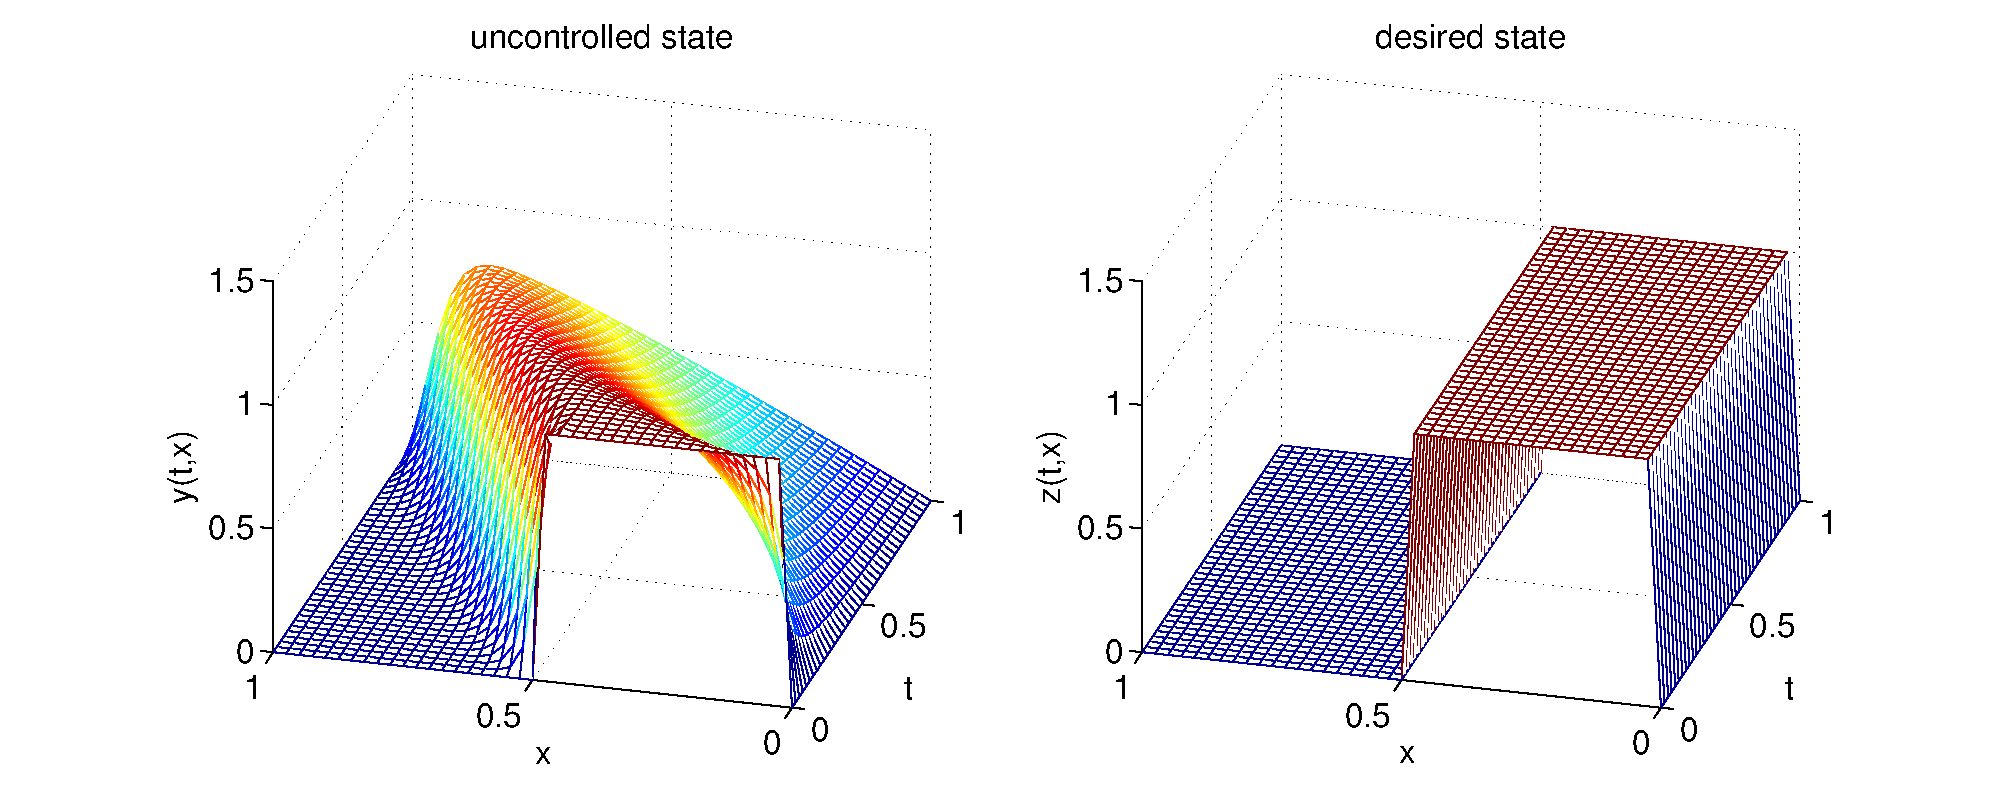
\includegraphics[width=0.9\textwidth]{plots/desiredState}
\caption{Uncontrolled and desired state for $\nu = 0.01$.}\label{desState}
\end{figure}
We now present a discretization of the cost functional \eqref{minJ} as well as Burgers' equation \eqref{Burgers2} which is again in conservative form as already seen in Section \ref{BurgersPODDEIM}. Therefore, we make the ansatz that the control $u$ can be approximated in a finite element way as the superposition of piecewise linear test functions $\phi_j$ as introduced in Appendix \ref{FEMDiscr_space}. This approach can be written as,
\begin{align}
 \label{ansatzu}
 u(t,x) \approx \sum_{j=1}^N u_j(t) \phi_j(x),
\end{align}
where $u_j$ are the respective coefficients of $\phi_j$ that only depend on time, see for example \cite{FEMbook}. Note, that this ansatz also implies that the control is zero at the boundary of $\Omega$ and, therefore, does not change the behavior of the solution $y$ at those points. Furthermore, we will choose $u(0,x) = 0$ as initial control which, again, does not affect the initial condition on $y$.

In order to discretize \eqref{minJ}, the outermost time integral has been approximated by a simple sum using a constant step size $\delta \! t$ for the discretization of the time interval $[0,T]$. We therefore obtain all time-dependent quantities at discrete time instances $t_i$, where $t_0 = 0$ and $t_{N_t} = T$. Recall, that in Appendix \ref{FEMDiscr_space} the state has been approximated in the following way, $y(t,x) \approx \sum_{j=1}^N y_j(t) \phi_j(x)$, a fully discrete version of the cost functional is given by,
\begin{align}
\label{minJ_discr}
\min_{\mathbf{u}_0,...,\mathbf{u}_{N_t}} \mathcal{J}(\mathbf{y}_0,...,\mathbf{y}_{N_t},\mathbf{u}_0,...,\mathbf{u}_{N_t}) = \min_{\mathbf{u}_0,...,\mathbf{u}_{N_t}} \sum_{i=0}^{N_t} \delta \! t \left(\frac{1}{2}\mathbf{y}_i^T M \mathbf{y}_i - \mathbf{z}^T \mathbf{y}_i + \frac{\omega}{2} \mathbf{u}_i^T M \mathbf{u}_i  \right),
\end{align}
where the vector-valued quantities
\begin{align*}
\mathbf{y}_i = \begin{pmatrix}y_1(t_i) \\ \vdots \\ y_N(t_i) \end{pmatrix} \in \mathbb{R}^N, \quad \mathbf{u}_i = \begin{pmatrix}u_1(t_i) \\ \vdots \\ u_N(t_i) \end{pmatrix} \in \mathbb{R}^N, \quad \text{ for }t_i \in [0,T]
\end{align*}
are introduced and $M$ is the mass matrix as defined in Appendix \ref{FEMDiscr_space}. Note, that in \eqref{minJ_discr} the constant and positive term
\begin{align*}
\frac{1}{2} \int_0^T \int_0^L z^2(t,x) \ dx \ dt
\end{align*}
has been neglected since it does not influence the position of the minimum with respect to $u$. This can lead to a negative value of the discrete objective function even though \eqref{minJ} is positive. Furthermore, we assume that the desired state $z$ does not depend on time. The vector $\mathbf{z}$ tested against the hat functions $\phi_j$ is therefore given by,
\begin{align}
\label{fullz}
\mathbf{z} = \begin{pmatrix} \int_0^L z(x) \phi_1(x) dx \\ \vdots \\ \int_0^L z(x) \phi_N(x) dx\\ \end{pmatrix} \approx h \begin{pmatrix} z(x_1) \\ \vdots \\ z(x_N)\\ \end{pmatrix}.
\end{align}
The discretization of Burgers' equation \eqref{Burgers2} with the control on the right-hand side has been obtained by a finite element approach in space and an implicit Euler method in time as described in Appendix \ref{FEMDiscr_space} and Appendix \ref{implEuler}, respectively. The resulting discrete constraint in the form $c(y,u) = 0$ is a vector-valued function with the components equal to,
\begin{align}
\label{Burgers2_discr}
c_{i+1}(\mathbf{y}_i,\mathbf{y}_{i+1},\mathbf{u}_{i+1}) \equiv \frac{1}{\delta \! t} M \mathbf{y}_{i+1} - \frac{1}{\delta \! t} M \mathbf{y}_i + \frac{1}{2} B \mathbf{y}_{i+1}^2 + \nu C \mathbf{y}_{i+1} - \mathbf{f} - M \mathbf{u}_{i+1} = 0,
\end{align}
where $i=0,...,N_t-1$ and the constraint is given by $c := [c_1,...,c_{N_t}]^T$ which is a function of the state and the control at all discrete time instances.

Note, that the only nonlinearity that remains is derived from the discretization of the convective term of Burgers' equation. We will denote this nonlinearity by,
\begin{align}
 \label{fullNonlin}
 \mathcal{N}(\mathbf{y}_{i+1}) := \frac{1}{2} B \mathbf{y}_{i+1}^2,
\end{align}
and point out the special treatment of the nonlinearity in the following application of the Newton-type method using adjoint techniques for the derivative computation as introduced in Section \ref{optAdj}.

Therefore, we first note that after discretization in space and time, the cost function \eqref{minJ_discr} together with the constraint \eqref{Burgers2_discr} fit the framework of \eqref{allgControl}. We can, thus, build the fully discretized Lagrangian function according to the definition \eqref{genLagr}. The discrete Lagrangian of the full-order model is given by,
\begin{align}
\label{discLag}
&\mathcal{L}(\mathbf{y}_0,...,\mathbf{y}_{N_t}, \mathbf{u}_0,...,\mathbf{u}_{N_t},\boldsymbol{\lambda}_1,...,\boldsymbol{\lambda}_{N_t}) \nonumber \\
&\ = \sum_{i=0}^{N_t} \delta \! t \left( \frac{1}{2} \mathbf{y}_i^T M \mathbf{y}_i - \mathbf{z}^T\mathbf{y}_i + \frac{\omega}{2} \mathbf{u}_i^T M \mathbf{u}_i \right) \nonumber \\
&\quad +  \sum_{i=0}^{N_t-1} \boldsymbol{\lambda}_{i+1}^T \left( \frac{1}{\delta \! t} M \mathbf{y}_{i+1} - \frac{1}{\delta \! t} M \mathbf{y}_i + \frac{1}{2} B \mathbf{y}_{i+1}^2 + \nu C \mathbf{y}_{i+1} - \mathbf{f} - M \mathbf{u}_{i+1}  \right),
\end{align}
where the adjoint variable $\boldsymbol{\lambda}_i$ at each time instance is a vector of dimension $N$.

In all our numerical test calculations, adjoints were used for the computation of gradients and Hessian-vector products. Therefore, we will next present how the adjoint Algorithms \ref{alg:Adj1} and \ref{alg:Adj2} have been applied to the discretized Burgers' equation \eqref{minJ_discr}-\eqref{Burgers2_discr}.
\subsection{Numerical results for a Newton-type method using adjoints}
\label{NumTests_Hess}
We want to apply the optimization Algorithm \ref{alg:Opt} in order to solve \eqref{minJ_discr} for $\mathbf{u}_0,...,\mathbf{u}_{N_t}$, when $\mathbf{y}_0,...,\mathbf{y}_{N_t}$ is the solution of \eqref{Burgers2_discr}. Therefore, we will need the corresponding Lagrangian function \eqref{discLag} as well as the gradient and the Hessian-times-vector product as described in the algorithms \ref{alg:Adj1} and \ref{alg:Adj2}, respectively. We will concentrate on the solution of the two adjoint equations and refer to Appendix \ref{FEMDiscr} for the numerical solution of Burgers' equation.

In the adjoint Algorithm \ref{alg:Adj1} that computes the gradient of the cost functional \eqref{minJ_discr}, we mostly need to compute partial derivatives of the constraint \eqref{Burgers2_discr} and the cost functional itself with respect to the control $u$ and the state variable $y$. Since both the constraint and the cost functional depend on the control and the state at all time instances, the respective variables we need to consider are of the size $N \cdot N_t$,
\begin{align*}
\mathbf{\underline u} := \begin{pmatrix} \mathbf{u}_0 \\ \vdots \\ \mathbf{u}_{N_t} \end{pmatrix} \in \mathbb{R}^{(N \cdot N_t) \times 1}, \quad \mathbf{\underline y} := \begin{pmatrix} \mathbf{y}_0 \\ \vdots \\ \mathbf{y}_{N_t} \end{pmatrix} \in \mathbb{R}^{(N \cdot N_t) \times 1}.
\end{align*}
Therefore, at every outer iteration of the optimization loop, we first need to solve Burgers' equation on the whole time interval. In Algorithm \ref{alg:Adj1_Burgers}, we summarize the application of Algorithm \ref{alg:Adj1} to the full-order discrete optimal control problem with Burgers' equation as an implicit constraint. Thereby, the adjoint equation \eqref{adjoint1} reduces to an ordinary differential equation in the adjoint variable. Note, that we first need to solve the terminal condition \eqref{AdjFullOrder_term} for $\boldsymbol{\lambda}_{N_t}$ and then solve the set of equations \eqref{AdjFullOrder} backwards in time. Given the solution of \eqref{AdjFullOrder_term}-\eqref{AdjFullOrder}, the gradient of the cost function with respect to the control $u$ can be obtained according to \eqref{grad}.
\begin{algorithm}[H]
\caption{Algorithm \ref{alg:Adj1} applied to the full-order discrete Burgers' equation}
\label{alg:Adj1_Burgers}
\begin{algorithmic}[1]
\STATE From the initial condition $\mathbf{y}_0$ and the current control $\mathbf{u}_1,...,\mathbf{u}_{N_t}$, solve Burgers' equation for $\mathbf{y}_1,...,\mathbf{y}_{N_t}$ as described in Appendix \ref{FEMDiscr}
\STATE The adjoint equation \eqref{adjoint1} reads:
\begin{subequations}
\begin{align}
\label{AdjFullOrder_term}
\left(\frac{1}{\delta \! t}M + \mathcal{N}'(\mathbf{y}_{N_t}) +  \nu C\right)^T \boldsymbol{\lambda}_{N_t} &= -\delta \! t( M \mathbf{y}_{N_t} - \mathbf{ z} )\\
\label{AdjFullOrder}
\left(\frac{1}{\delta \! t}M + \mathcal{N}'(\mathbf{y}_{i}) + \nu C\right)^T \boldsymbol{\lambda}_i &= - (-\frac{1}{\delta \! t} M)^T \boldsymbol{\lambda}_{i+1} -\delta \! t( M \mathbf{y}_{i} - \mathbf{ z} ), \quad i = N_t-1,...,1
\end{align}
\end{subequations}
\STATE The gradient is computed according to formula \eqref{grad}:
\begin{align}
\label{gradFullOrder}
\nabla_u \hat{\mathcal J}(\mathbf{u}_0,...,\mathbf{u}_{N_t}) = \begin{pmatrix} \delta \! t \omega M \mathbf{u}_0 \\ \delta \! t \omega M \mathbf{u}_1 - M^T \boldsymbol{\lambda}_1 \\ \vdots \\ \delta \! t \omega M \mathbf{u}_{N_t} - M^T \boldsymbol{\lambda}_{N_t} \end{pmatrix}
\end{align}
\end{algorithmic}
\end{algorithm}
In \eqref{AdjFullOrder_term} and \eqref{AdjFullOrder} it is necessary to compute the first derivative of the nonlinear term \eqref{fullNonlin}. For an arbitrary vector $\mathbf{y} = [y_1,...,y_N]^T$ and a matrix $B \in \mathbb{R}^{N \times N}$, the first derivative of the nonlinear term $\mathcal{N}(\cdot)$ is given by,
\begin{align*}
\mathcal{N}'(\mathbf{y}) = \frac{d}{d\mathbf{y}}\left( \frac{1}{2} B \mathbf{y}^2 \right) = \begin{pmatrix} B_{1,1}y_1 & \hdots & B_{1,N}y_N \\
                                   B_{2,1}y_1 & \hdots & B_{2,N}y_N \\
                                      \vdots  &        &     \vdots \\
                                   B_{N,1}y_1 & \hdots & B_{N,N}y_N \end{pmatrix} \in \mathbb{R}^{N \times N},
\end{align*}
which is again an $N \times N$ matrix.

In order to solve the Newton equation \eqref{Newtoneqn_J} we also need to compute the Hessian $\nabla^2 \hat{\mathcal J}(u)$. Since this is a matrix of dimension $N \cdot N_t \times N \cdot N_t$, we solve the linear system \eqref{Newtoneqn_J} with the truncated CG method where we only need to compute the product of the Hessian times a vector and never need to store the whole Hessian matrix, see Algorithm \ref{alg:serCG}. In Algorithm \ref{alg:Adj2_Burgers}, we present the application of the general Hessian-times-vector computation as derived in Section \ref{Hessadj} to the optimization of Burgers' equation. Therefore, we define the arbitrary vector $\mathbf{\underline v} := (\mathbf{v}^T_0, ..., \mathbf{v}^T_{N_t} )^T$ and derive the equations \eqref{wFullOrder_init}-\eqref{wFullOrder} and \eqref{pFullOrder_term}-\eqref{pFullOrder} for the auxiliary variables $w$ and $p$ according to the respective general formulas \eqref{eqnw} and \eqref{eqnp}. It is important to note that the initial condition \eqref{wFullOrder_init} and the terminal condition \eqref{pFullOrder_term} follow directly from the general equations \eqref{eqnw} and \eqref{eqnp} when the respective partial derivative is computed.
\newpage
\begin{algorithm}[H]
\caption{Algorithm \ref{alg:Adj2} applied to the full-order discrete Burgers' equation}
\label{alg:Adj2_Burgers}
\begin{algorithmic}[1]
\STATE We assume that we have already computed $\mathbf{y}_0,...,\mathbf{y}_{N_t}, \mathbf{u}_0,...,\mathbf{u}_{N_t},\boldsymbol{\lambda}_1,...,\boldsymbol{\lambda}_{N_t}$ in \mbox{Algorithm \ref{alg:Adj1_Burgers}}
\STATE Equation \eqref{eqnw} reads:
\begin{subequations}
\begin{align}
\label{wFullOrder_init}
\mathbf{w}_0 &= 0 \\
\label{wFullOrder}
\left( \frac{1}{\delta \! t}M + \mathcal{N}'(\mathbf{y}_{i+1}) + \nu C \right) \mathbf{w}_{i+1} &= - (-\frac{1}{\delta \! t} M) \mathbf{w}_i - M\mathbf{v}_{i+1} , \quad i = 0,...,N_t-1
\end{align}
\end{subequations}
\STATE Equation \eqref{eqnp} reads:
\begin{subequations}
\begin{align}
\label{pFullOrder_term}
\left( \frac{1}{\delta \! t}M + \mathcal{N}'(\mathbf{y}_{N_t}) + \nu C \right)^T \mathbf{p}_{N_t} &= \delta \! t M \mathbf{w}_{N_t} + \text{diag}(\boldsymbol{\lambda}^T_{N_t} b_1,...,\boldsymbol{\lambda}^T_{N_t} b_N) \mathbf{w}_{N_t}\\
\label{pFullOrder}
\left( \frac{1}{\delta \! t}M + \mathcal{N}'(\mathbf{y}_{i}) + \nu C \right)^T \mathbf{p}_{i} &= - (-\frac{1}{\delta \! t} M)^T \mathbf{p}_{i+1} + \delta \! t M \mathbf{w}_{i} \nonumber \\
&\quad + \text{diag}(\boldsymbol{\lambda}^T_{i} b_1,...,\boldsymbol{\lambda}^T_{i} b_N) \mathbf{w}_{i}, \quad i = N_t-1,...,1
\end{align}
\end{subequations}
\STATE The Hessian times a vector $\mathbf{\underline v}$ is computed according to formula \eqref{hesseqn}:
\begin{align}
\label{HessFullOrder}
\nabla^2 \hat{\mathcal J}(\mathbf{u}_0,...,\mathbf{u}_{N_t}) \cdot \mathbf{\underline v} = \begin{pmatrix} \delta \! t \omega M \mathbf{v}_0 \\ -M^T \mathbf{p}_1 + \delta \! t \omega M \mathbf{v}_1\\ \vdots \\ -M^T \mathbf{p}_{N_t} + \delta \! t \omega M \mathbf{v}_{N_t} \end{pmatrix}
\end{align}
\end{algorithmic}
\end{algorithm}
Note that in \eqref{pFullOrder_term}-\eqref{pFullOrder} as well as in \eqref{HessFullOrder} it is necessary to compute second partial derivatives of the Lagrangian function. Therefore, we first note that due to the definition of the Lagrangian, mixed second order derivatives vanish. Furthermore, we present the analytic computation of the second partial derivative of the quantity $\boldsymbol{\lambda}^T \mathcal{N}(\mathbf{y})$ with respect to the state variable $\mathbf{y}$,
\begin{align*}
\frac{d^2}{d\mathbf{y}^2} \left( \boldsymbol{\lambda}^T \mathcal{N}(\mathbf{y}) \right) \mathbf{w} &= \frac{d^2}{d\mathbf{y}^2} \left( \boldsymbol{\lambda}^T (\frac{1}{2} B \mathbf{y}^2) \right) \mathbf{w}
= \frac{d^2}{d\mathbf{y}^2} \left( \frac{1}{2} \sum_{k=1}^N \lambda_k \sum_{j=1}^N B_{k,j}y_j^2 \right) \mathbf{w} \\
&= \frac{d}{d\mathbf{y}}\begin{pmatrix} \sum_{k=1}^N \lambda_k B_{k,1}y_1 \\ \vdots \\ \sum_{k=1}^N \lambda_k B_{k,N}y_N \end{pmatrix} \mathbf{w}
= \begin{pmatrix} \sum_{k=1}^N \lambda_k B_{k,1} & & \\ & \ddots & \\ & & \sum_{k=1}^N \lambda_k B_{k,N}\end{pmatrix}\mathbf{w} \\
&= \text{diag}(\boldsymbol{\lambda}^T b_1,...,\boldsymbol{\lambda}^T b_N) \mathbf{w},
\end{align*}
where $\boldsymbol{\lambda} = (\lambda_1,...,\lambda_N)^T$, $\mathbf{y} = (y_1,..,y_N)^T$ ,and $b_1,...,b_N$ are the columns of the matrix $B$ such that $B = (b_1 |... | b_N)$.

Figures \ref{optFull} and \ref{optFullu} show numerical results of Algorithm \ref{alg:Opt} applied to problem \eqref{minJ_discr} with implicit constraint \eqref{Burgers2_discr}. In the considered setting, we chose $\nu = 0.01$ in Burgers' equation, $\omega = 0.005$ for the control penalty, and $N = N_t = 80$ grid points in time and space. In order to be able to perform the optimization Algorithm \ref{alg:Opt} using Armijo line search as described in Algorithm \ref{alg:Armijo} and the gradient and Hessian-vector product computation in Algorithms \ref{alg:Adj1_Burgers} and \ref{alg:Adj2_Burgers}, respectively, we need to specify some settings which have been summarized in Table \ref{params}. Also the Newton iteration for the numerical solution of Burgers' equation requires to set some tolerances.
\begin{table}[H]
\centering
\begin{tabular}{|c|c|c|c|c|c|c|}
  \hline
  $\varepsilon_\mathcal{J}$ & $\varepsilon_\nabla$ & $\varepsilon_\alpha$ & $\alpha_{min}$ & $\eta_k$ & $\varepsilon_{Newton}$ & \texttt{max\_newton} \\
  \hline
  \texttt{10e-8} & \texttt{10e-9} & \texttt{10e-4} & \texttt{10e-8} & \texttt{10e-2} & \texttt{10e-3} & \texttt{20} \\
  \hline
\end{tabular}
\caption{Choice of parameters for the numerical results in Figure \ref{optFull} and \ref{optFullu}.}\label{params}
\end{table}
The outer optimization loop of algorithm \ref{alg:Opt} stops when either the value of the objective function does not change anymore ($\varepsilon_\mathcal{J}$ in Algorithm \ref{alg:Opt}) or the zero-gradient condition is fulfilled up to a certain precision ($\varepsilon_\nabla$ in Algorithm \ref{alg:Opt}). The tolerance of the Armijo line  search is set by $\varepsilon_\alpha$ and a minimum step length is guaranteed by $\alpha_{min}$, see Algorithm \ref{alg:Armijo}. The truncated CG-algorithm \ref{alg:serCG} is terminated by the choice of $\eta_k$, and $\varepsilon_{Newton}$ and \texttt{max\_newton} are, respectively, the tolerance and the maximum number of iterations of Newton's method as described in Algorithm \ref{alg:Euler}.

From the numerical results in Figure \ref{optFull}, we see that the state variable $y$ converges to the desired state $z$ as the number of optimization iterations $k$ increases. For the presented setting, after $6$ iterations a state has been reached such that the value of the objective function \eqref{minJ_discr} does not decrease any further than \texttt{0.024}.
\begin{figure}[H]
\centering
\subfloat[$k=0$ (uncontrolled)]{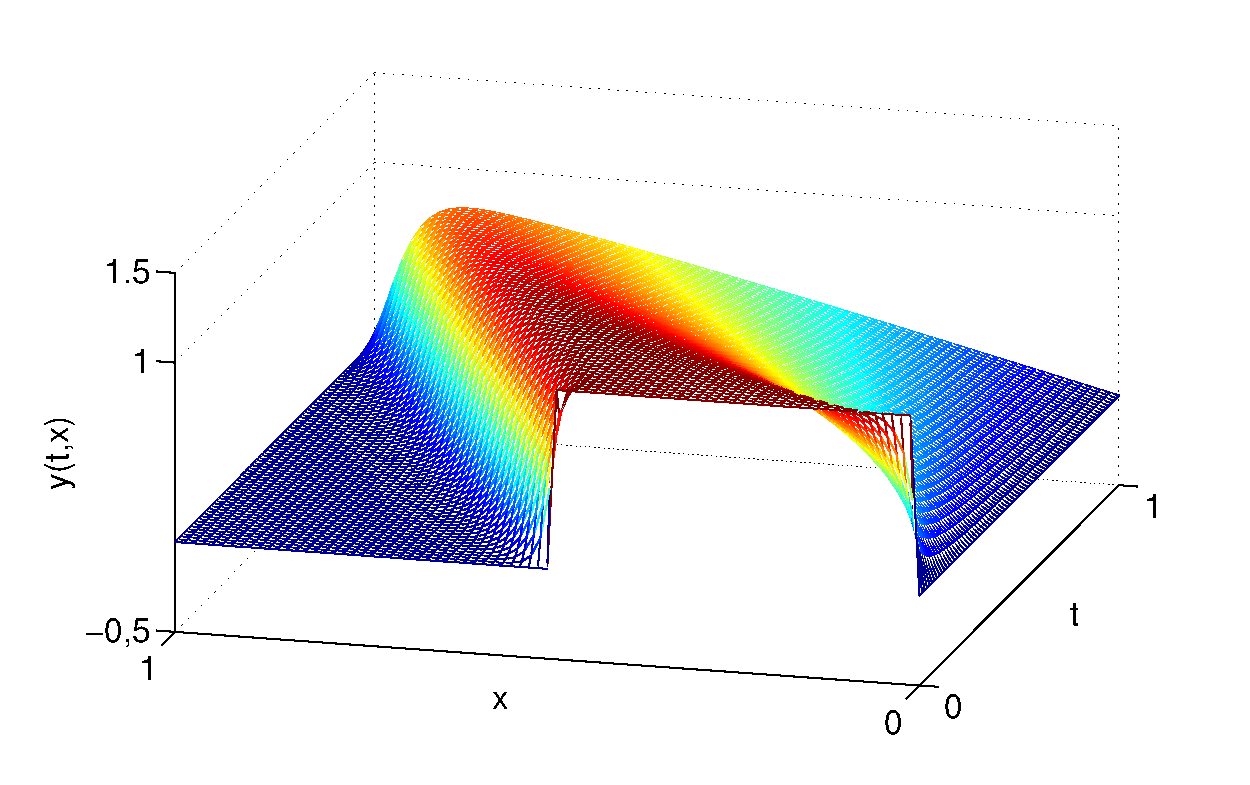
\includegraphics[width=0.33\textwidth]{plots/controlFullk0_new}}\hfill
\subfloat[$k=1$ ]{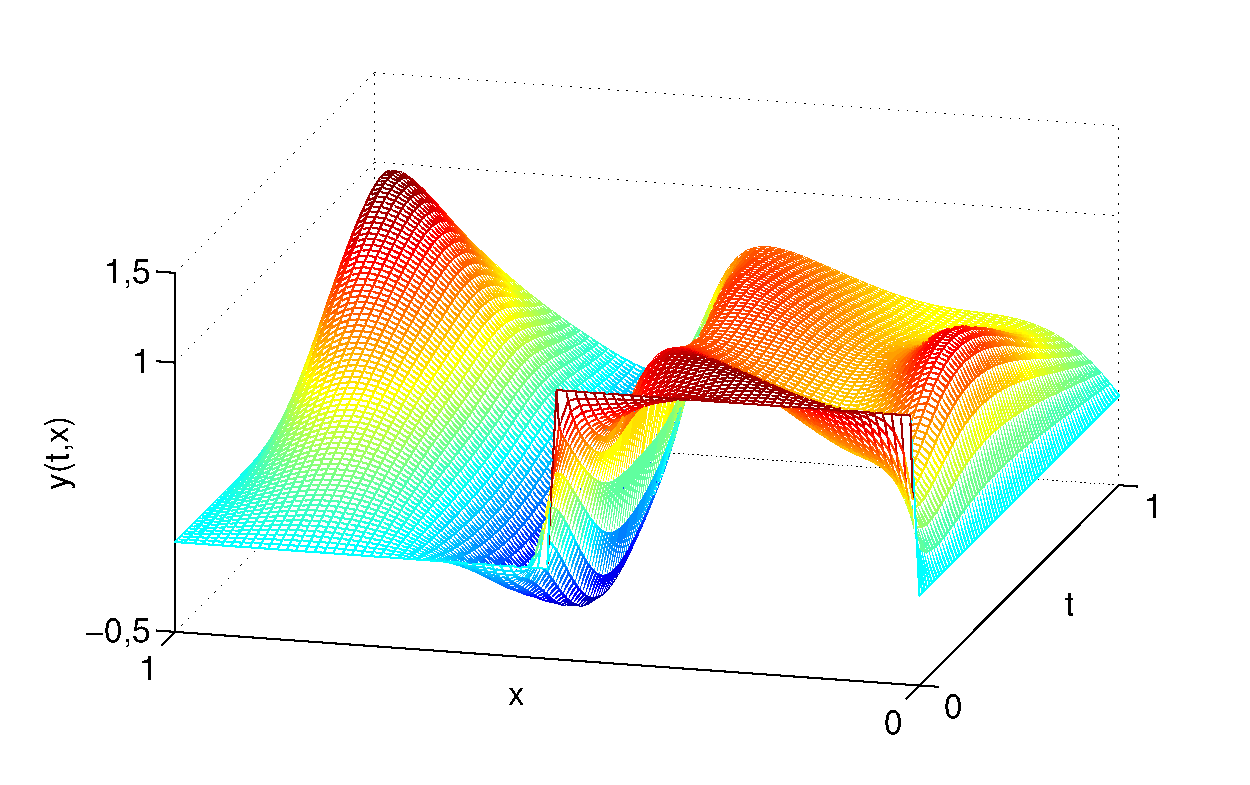
\includegraphics[width=0.33\textwidth]{plots/controlFullk1_new}}\hfill
\subfloat[$k=2$]{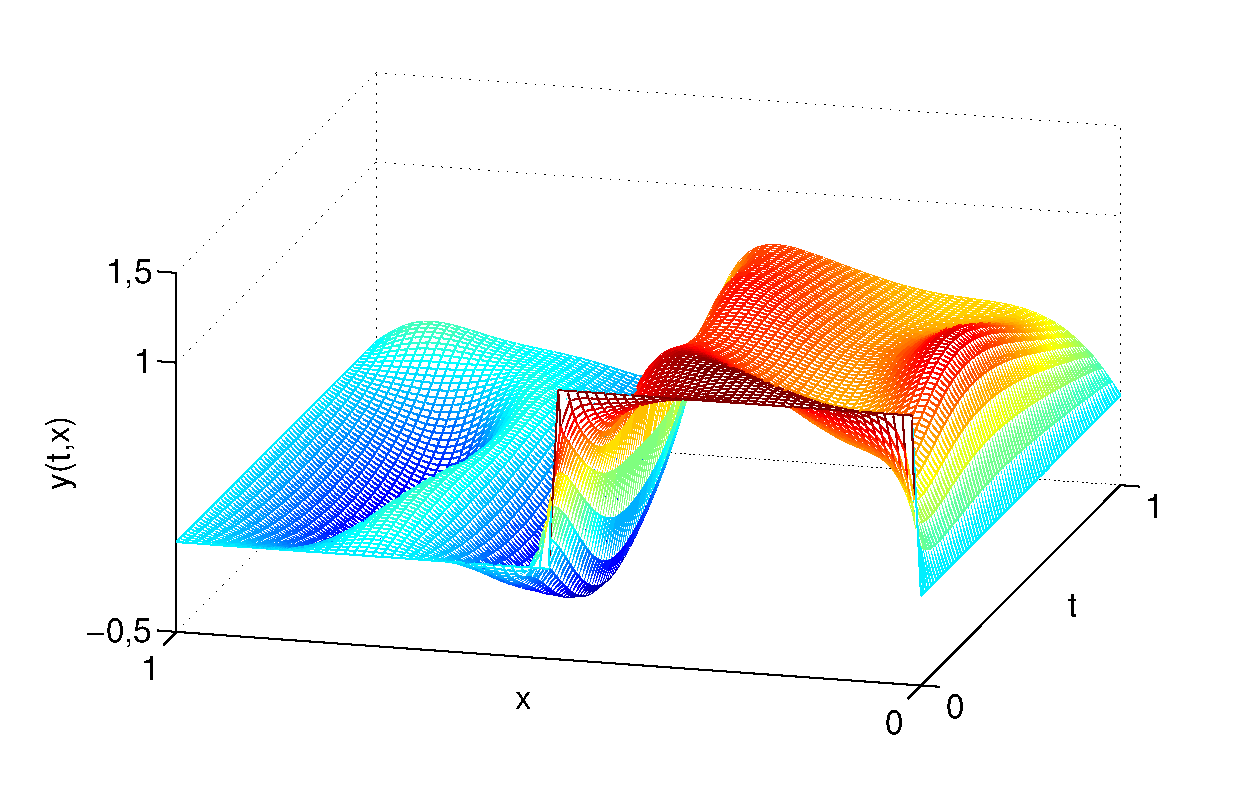
\includegraphics[width=0.33\textwidth]{plots/controlFullk2_new}}\\
\subfloat[$k=3$ ]{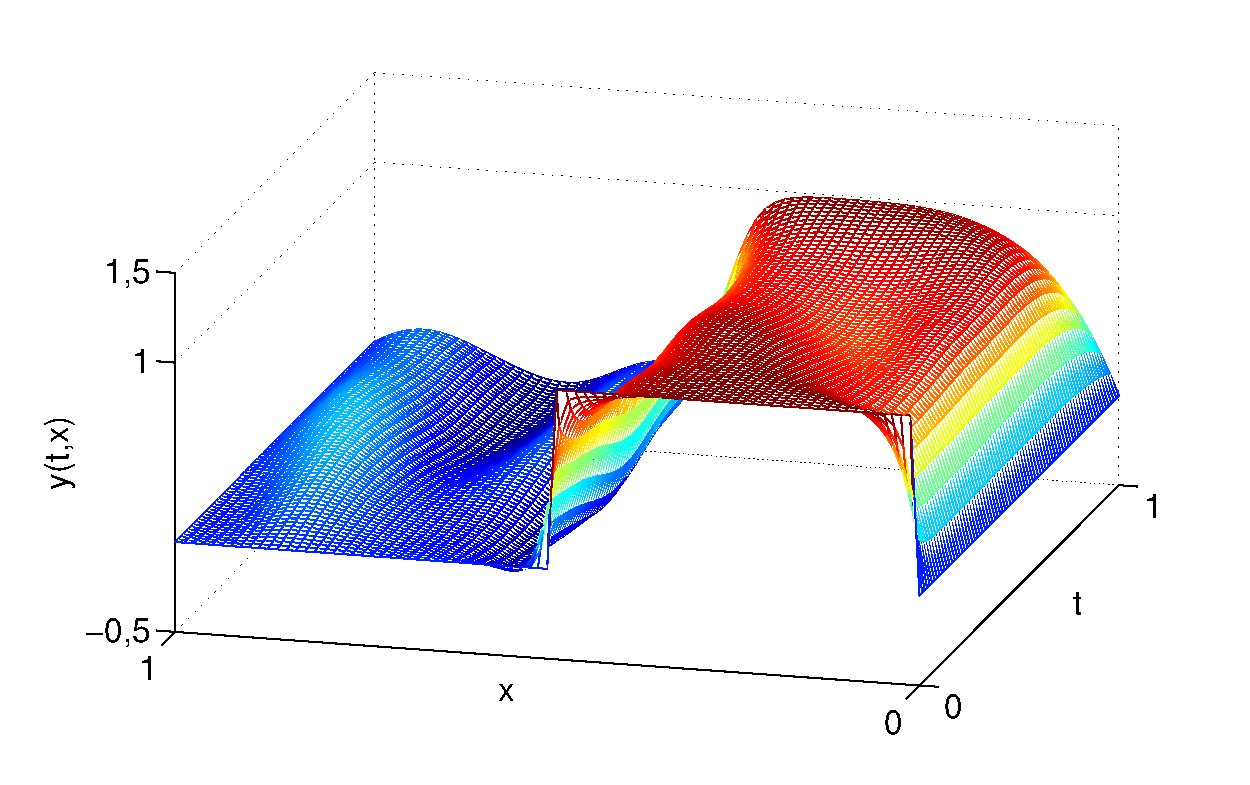
\includegraphics[width=0.33\textwidth]{plots/controlFullk3_new}}\hfill
\subfloat[$k=4$ ]{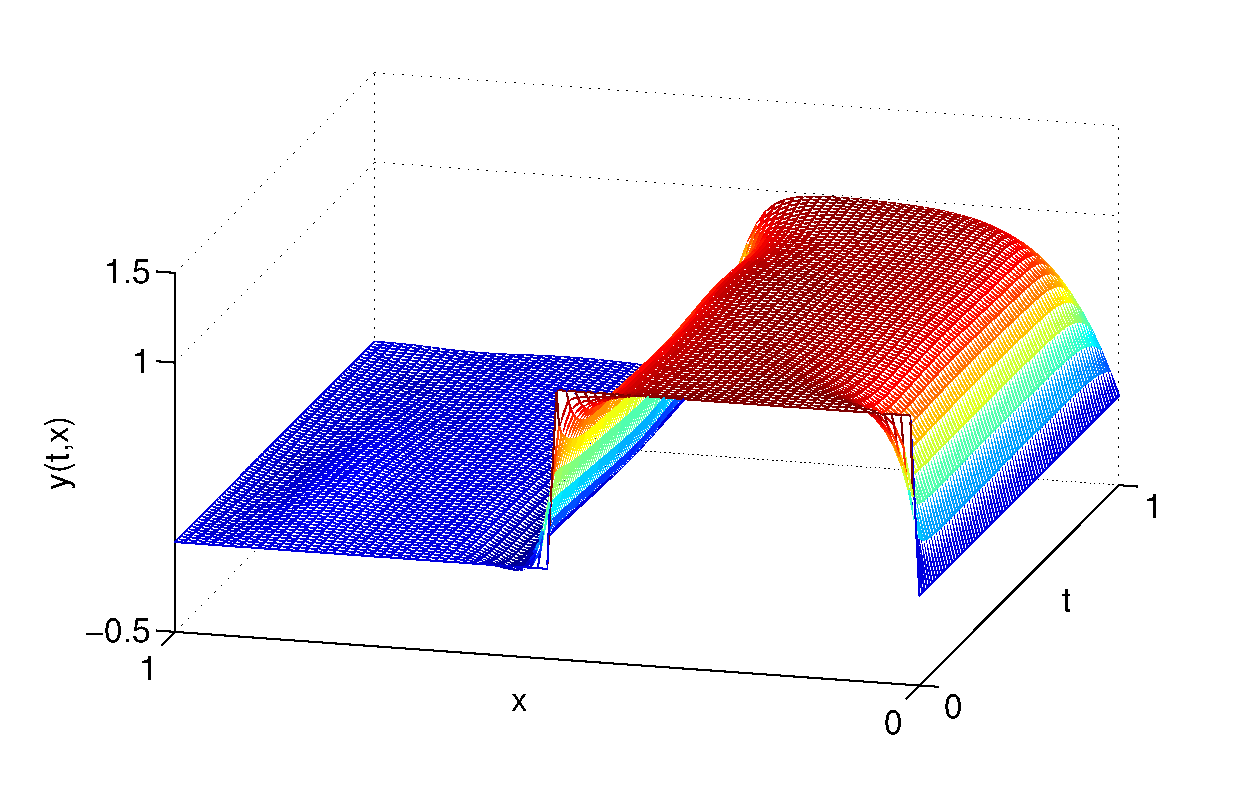
\includegraphics[width=0.33\textwidth]{plots/controlFullk4_new}}\hfill
\subfloat[$k=5$]{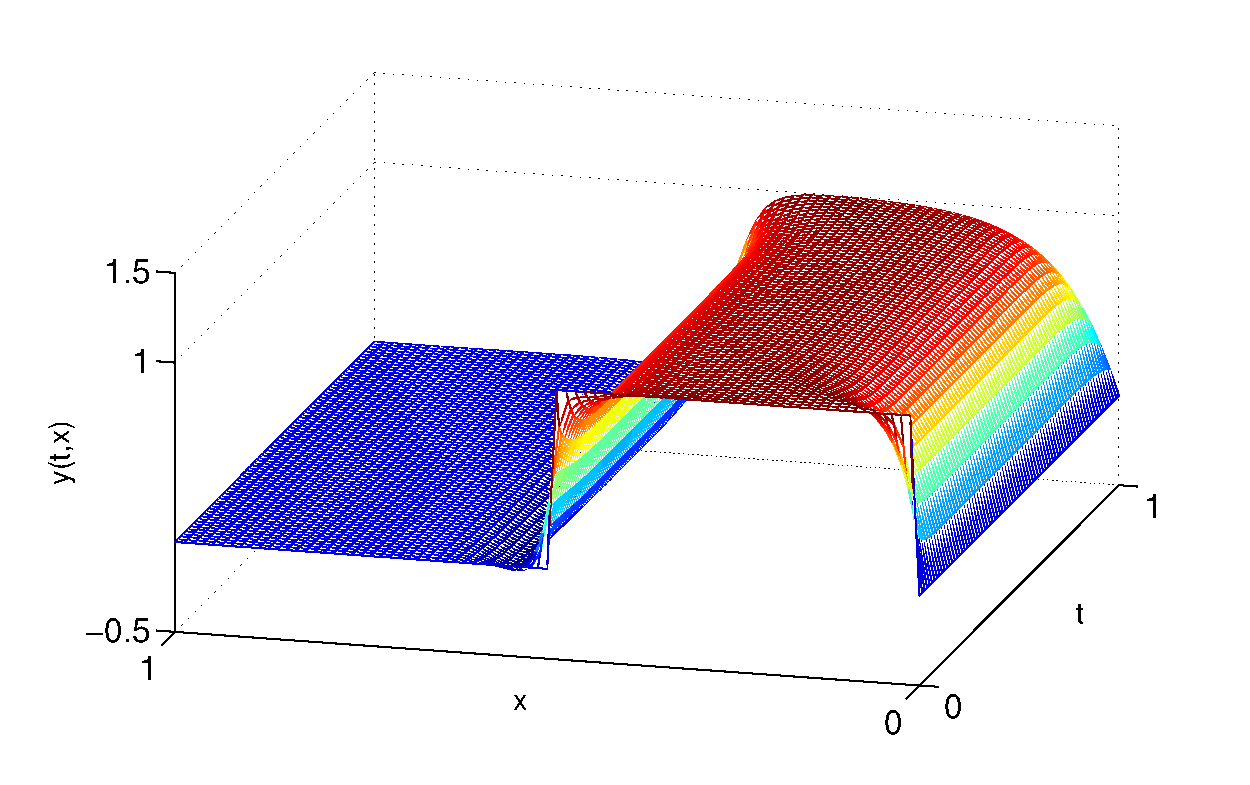
\includegraphics[width=0.33\textwidth]{plots/controlFullk5_new}}\\
\caption{The state $y$ at different stages $k$ of the optimization iteration.}\label{optFull}
\end{figure}
In Figure \ref{optFullu}, we present the control that corresponds to the states presented before. After convergence, we see in the last plot of Figure \ref{optFullu} the desired optimal control $u^*$ that drives the solution to Burgers' equation into the desired state $z$, i.e. minimizes the cost function.
\begin{figure}[H]
\centering
\subfloat[$k=0$ (initial)]{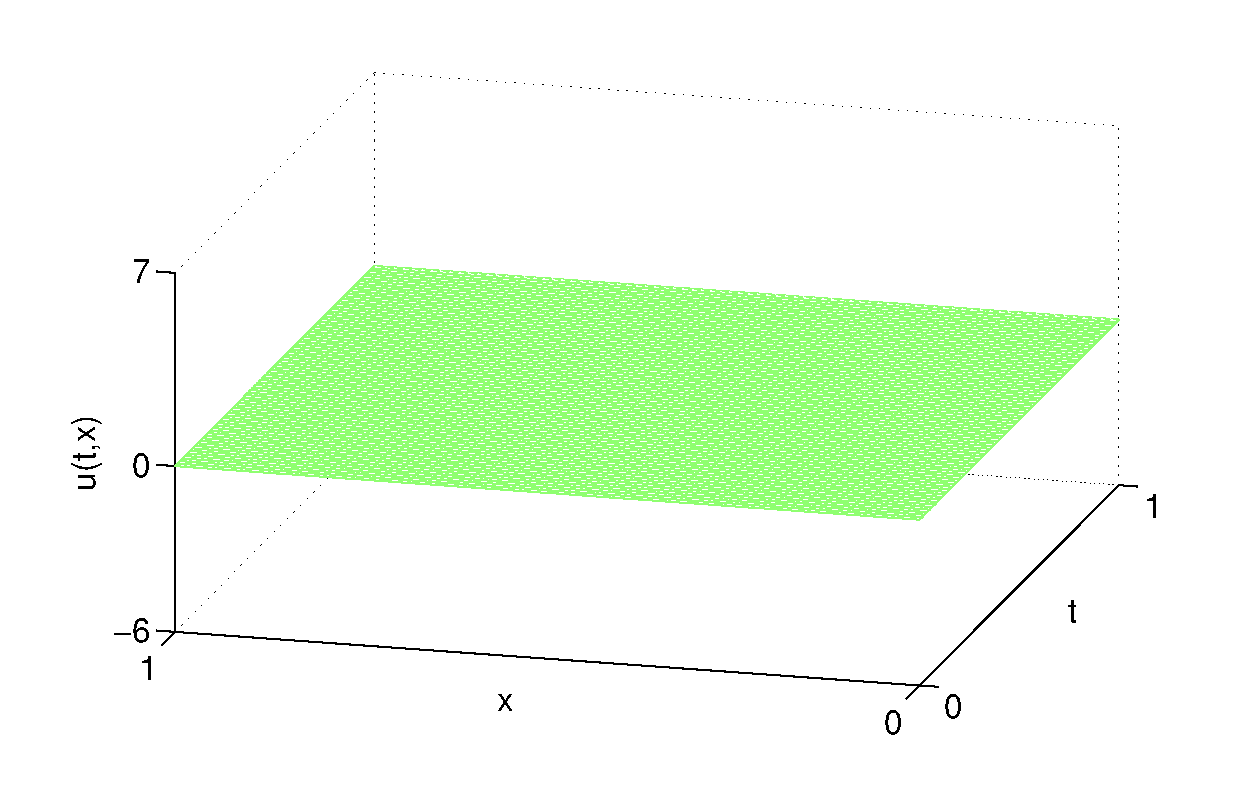
\includegraphics[width=0.33\textwidth]{plots/uFullk0_new}}\hfill
\subfloat[$k=1$ ]{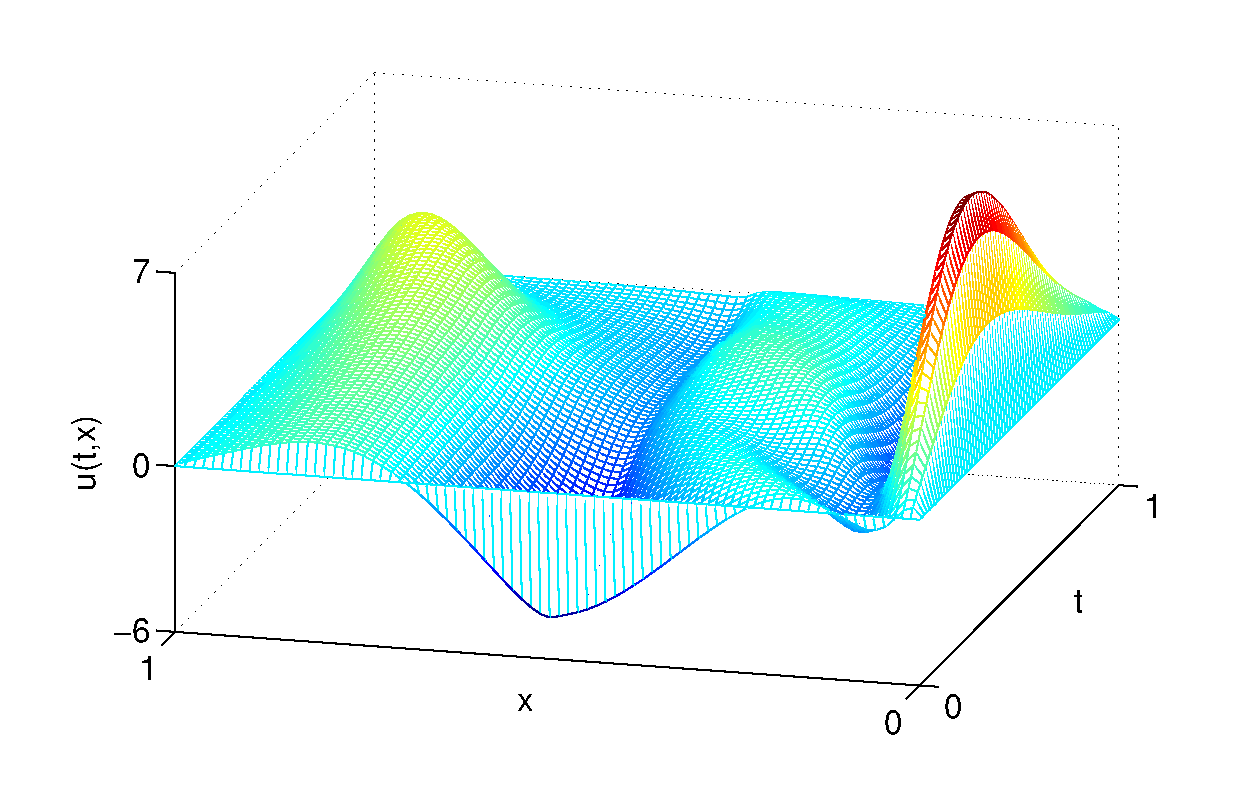
\includegraphics[width=0.33\textwidth]{plots/uFullk1_new}}\hfill
\subfloat[$k=2$]{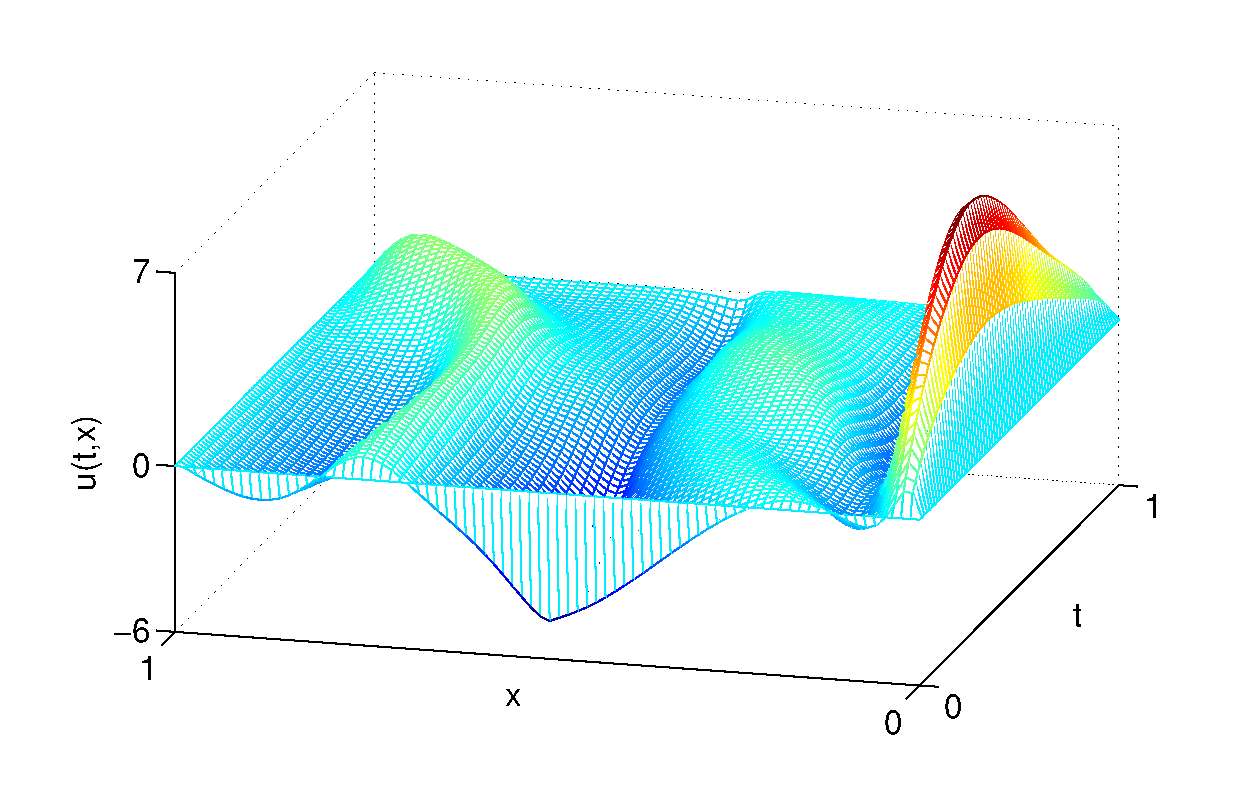
\includegraphics[width=0.33\textwidth]{plots/uFullk2_new}}\\
\subfloat[$k=3$ ]{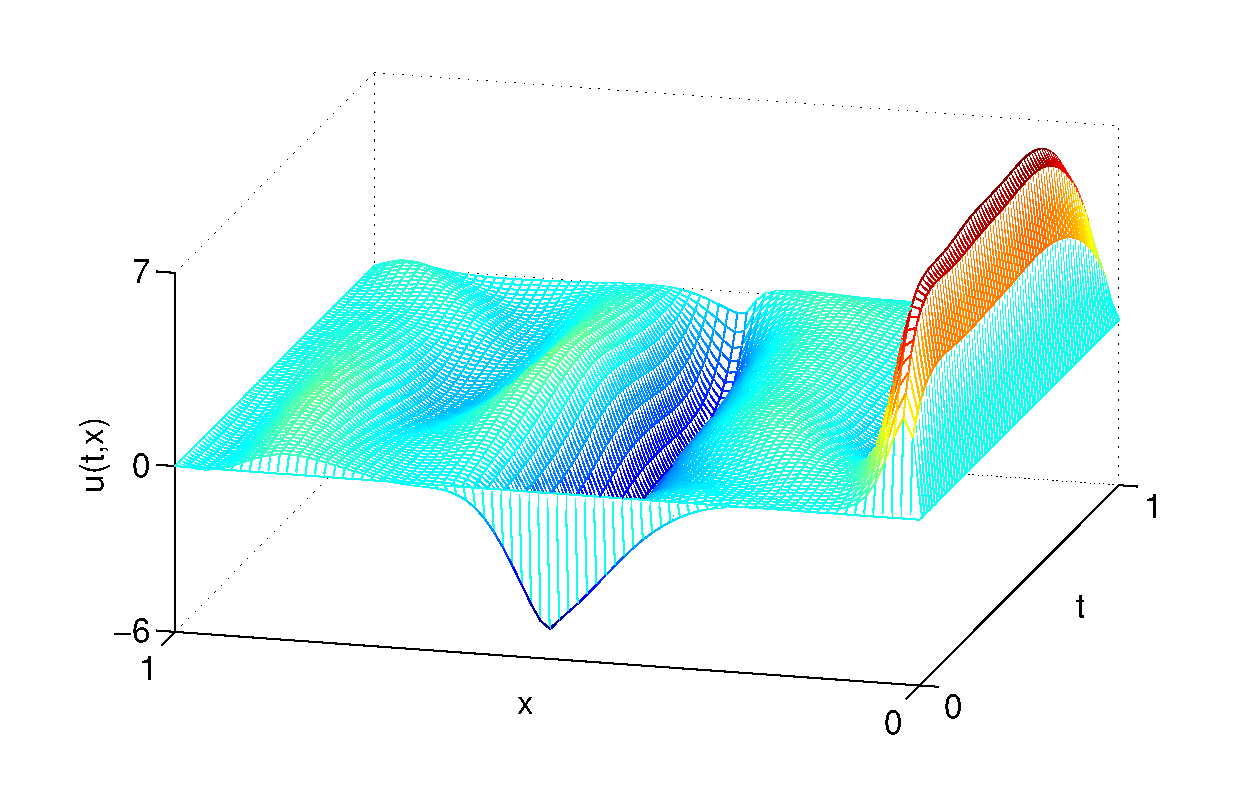
\includegraphics[width=0.33\textwidth]{plots/uFullk3_new}}\hfill
\subfloat[$k=4$ ]{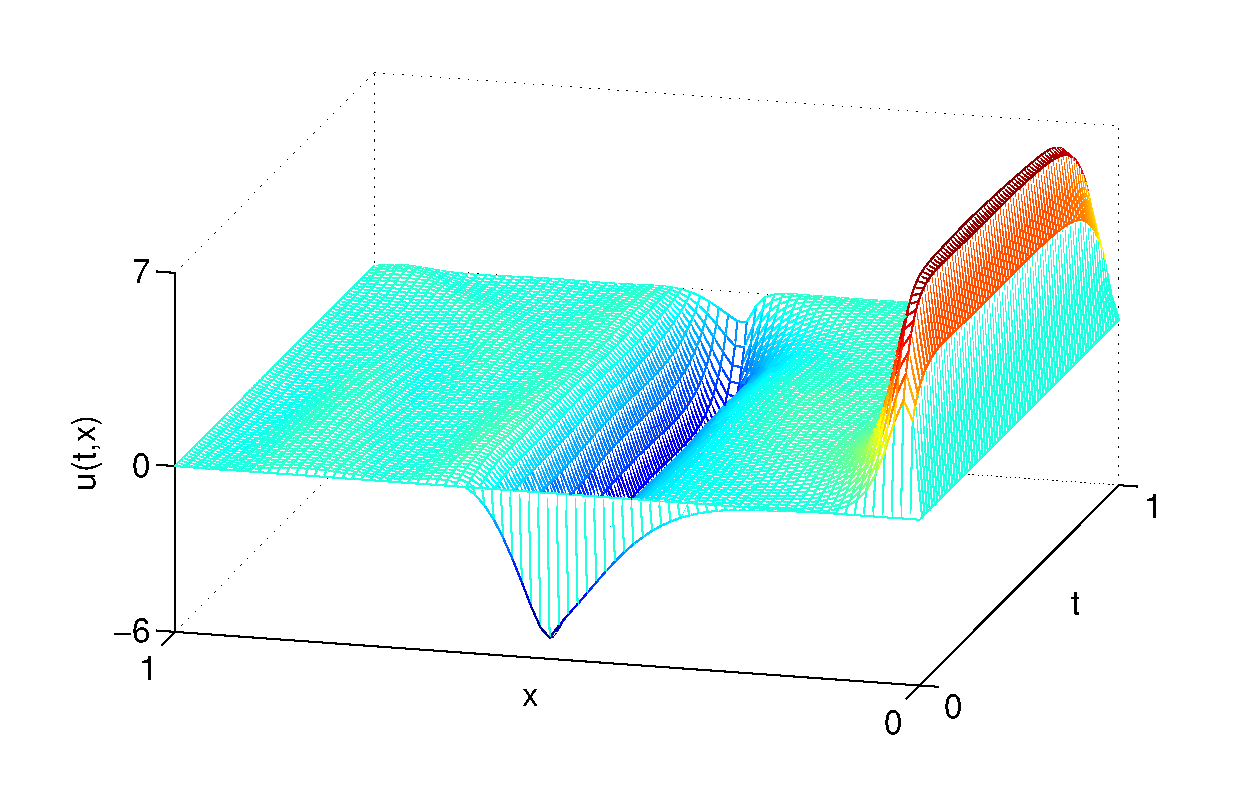
\includegraphics[width=0.33\textwidth]{plots/uFullk4_new}}\hfill
\subfloat[$k=5$]{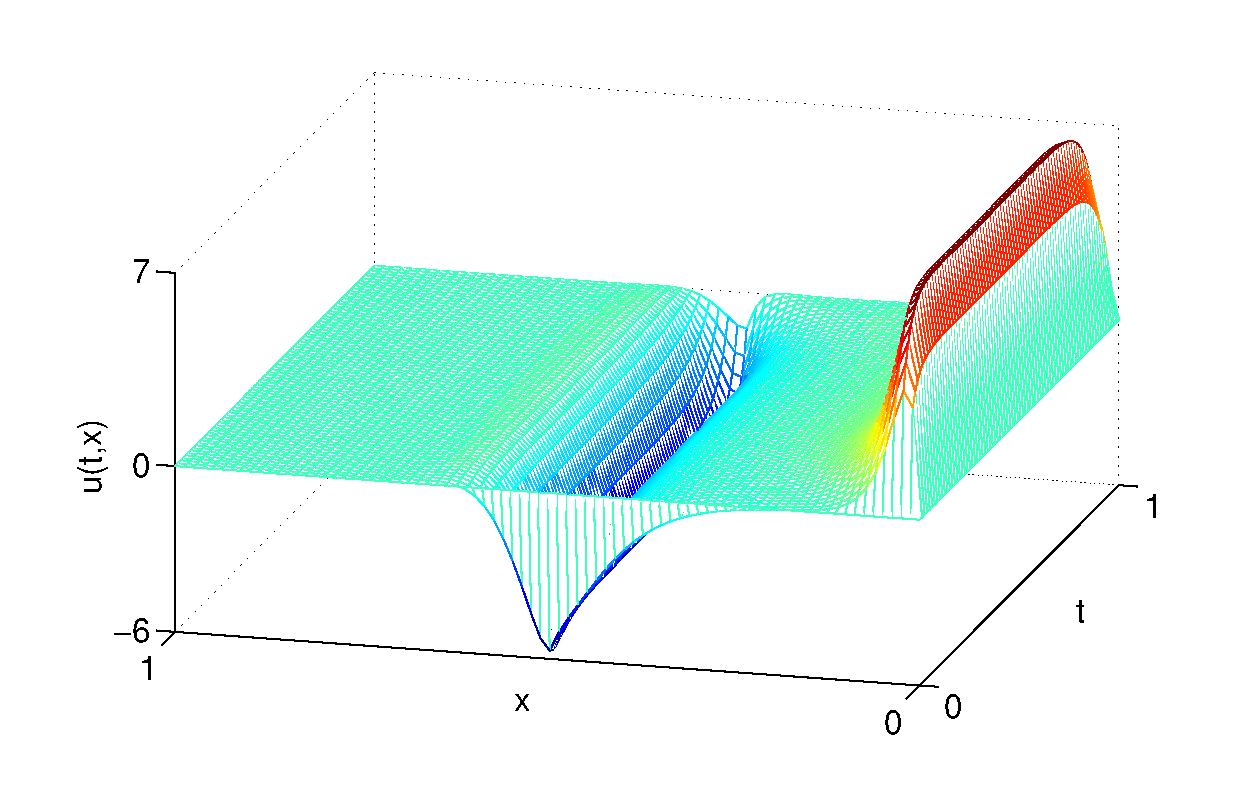
\includegraphics[width=0.33\textwidth]{plots/uFullk5_new}\label{optFullu_opt}}\\
\caption{The control $u$ at different stages $k$ of the optimization iteration.}\label{optFullu}
\end{figure}
A second numerical test using the same parameters as in Table \ref{params} has been performed in order to show the dependence of the optimization algorithm on the control penalty $\omega$. From \eqref{minJ} we see that the smaller we choose $\omega$ the more we put emphasis on driving the state $y$ into the desired state and allow a large control.
\begin{figure}[H]
\centering
\subfloat{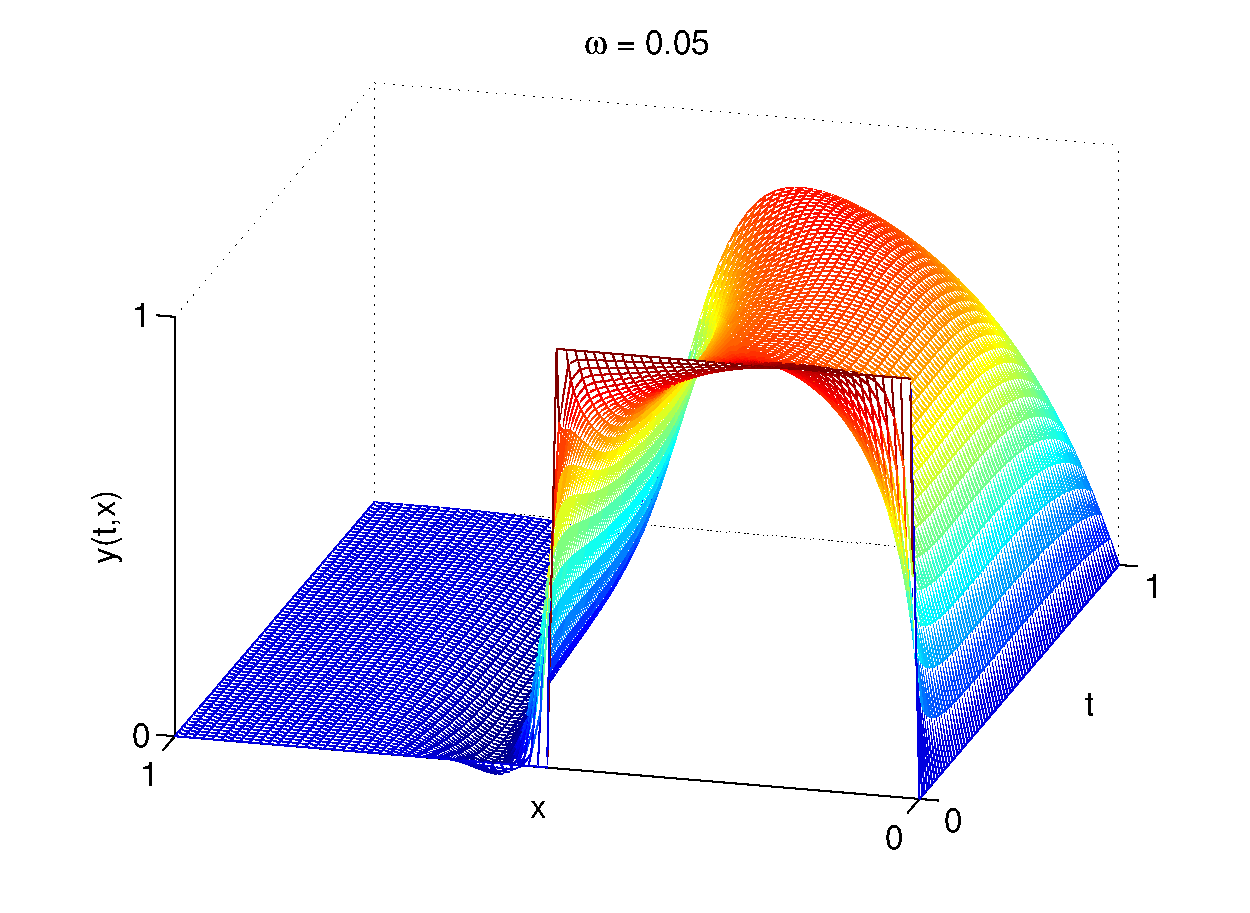
\includegraphics[width=0.33\textwidth]{plots/y_w05}}\hfill
\subfloat{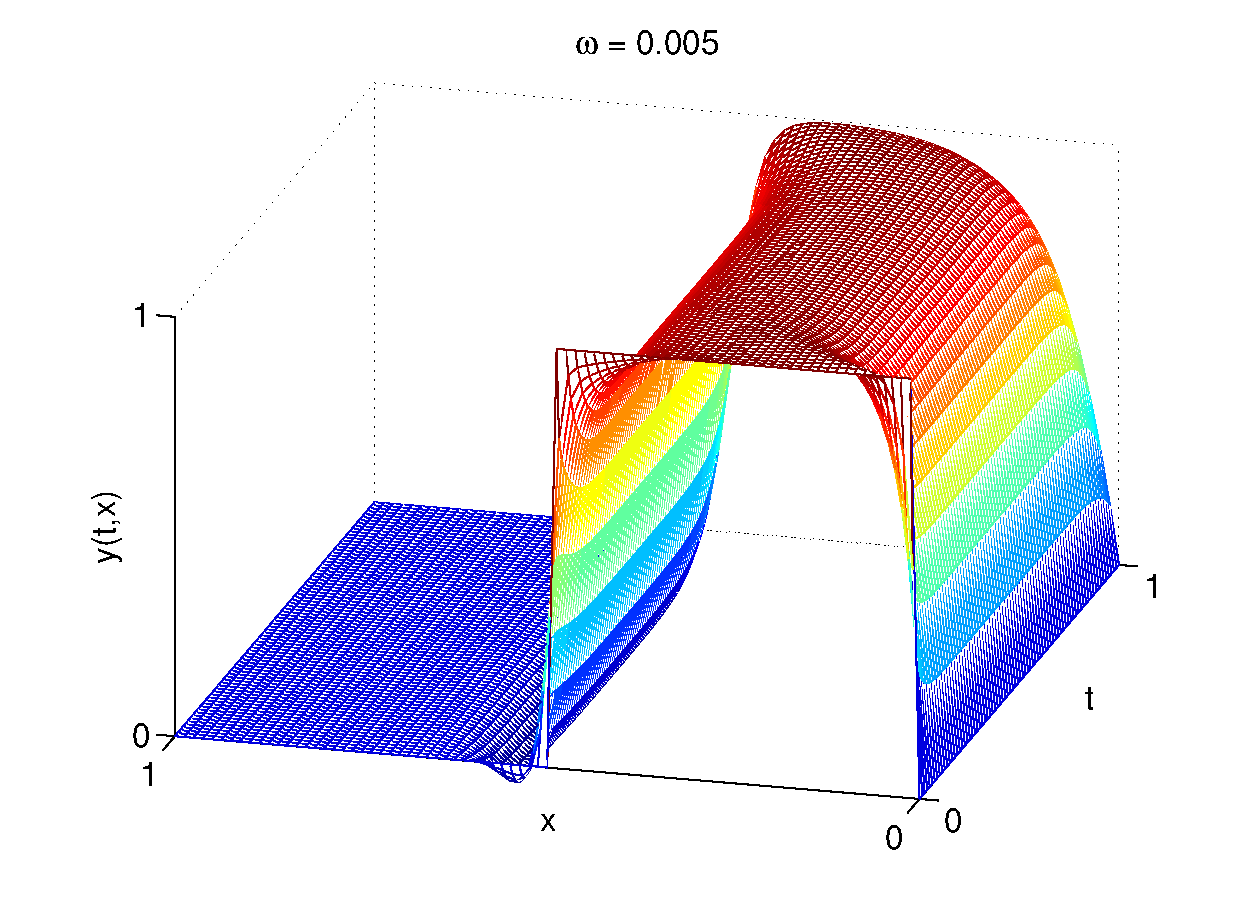
\includegraphics[width=0.33\textwidth]{plots/y_w005}}\hfill
\subfloat{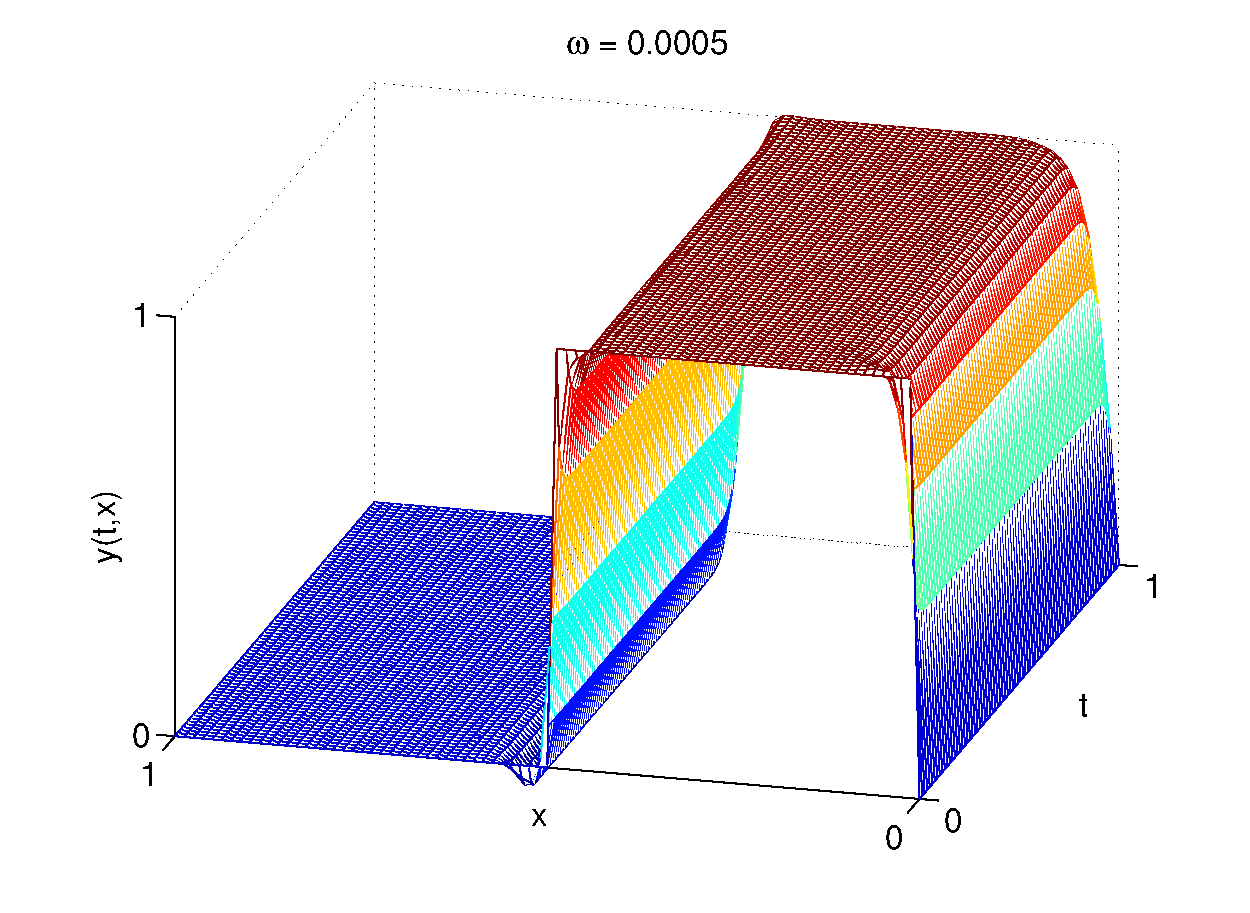
\includegraphics[width=0.33\textwidth]{plots/y_w0005}}\\
\subfloat{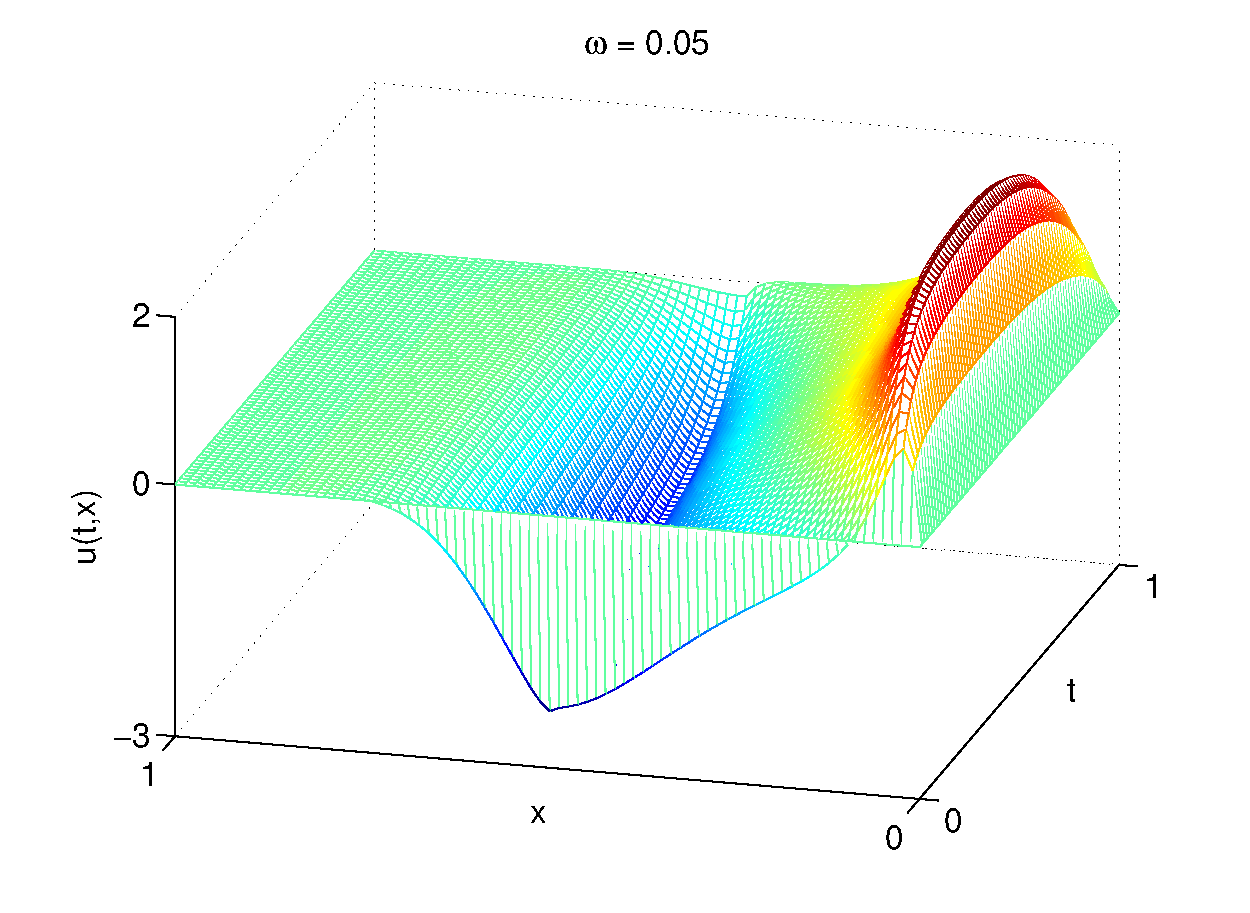
\includegraphics[width=0.33\textwidth]{plots/u_w05}}\hfill
\subfloat{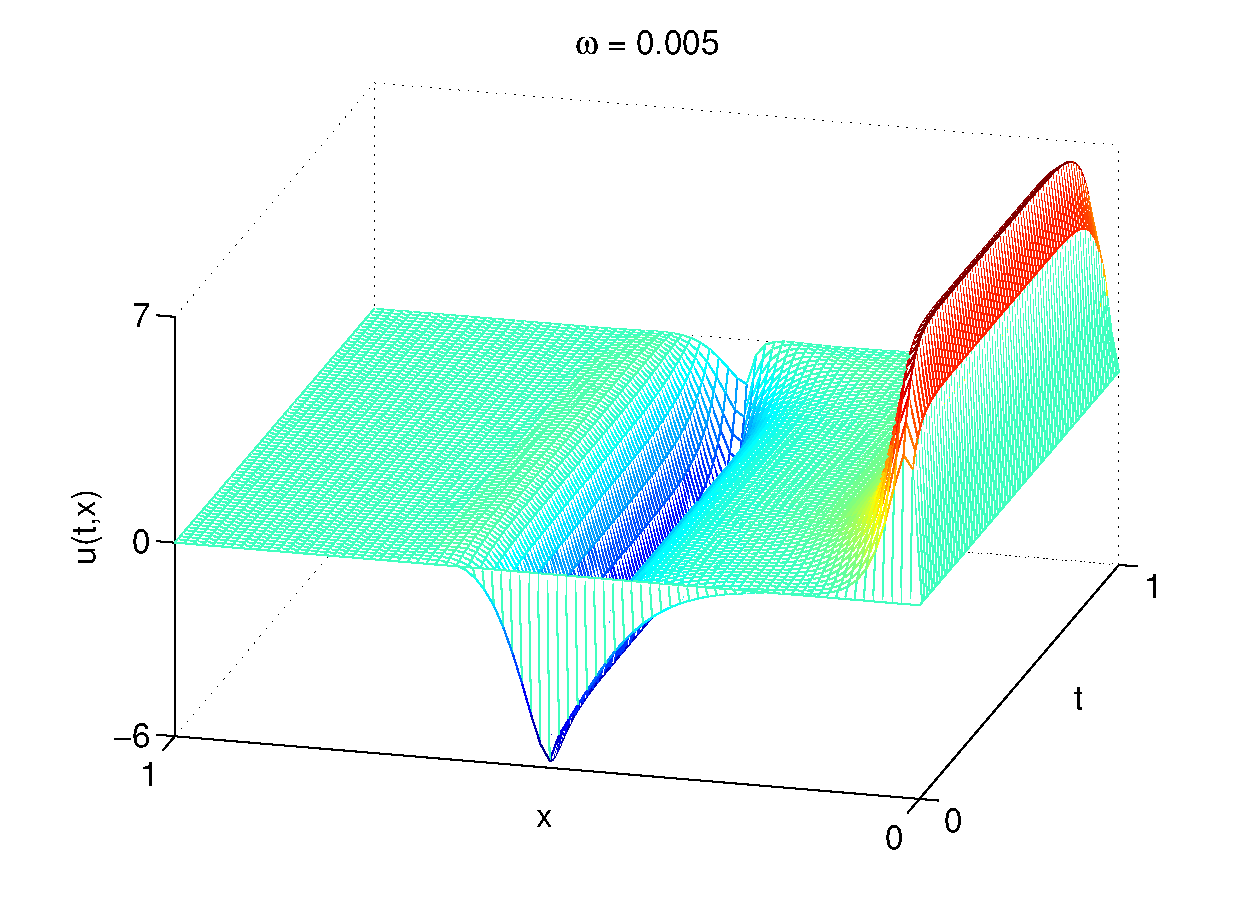
\includegraphics[width=0.33\textwidth]{plots/u_w005}}\hfill
\subfloat{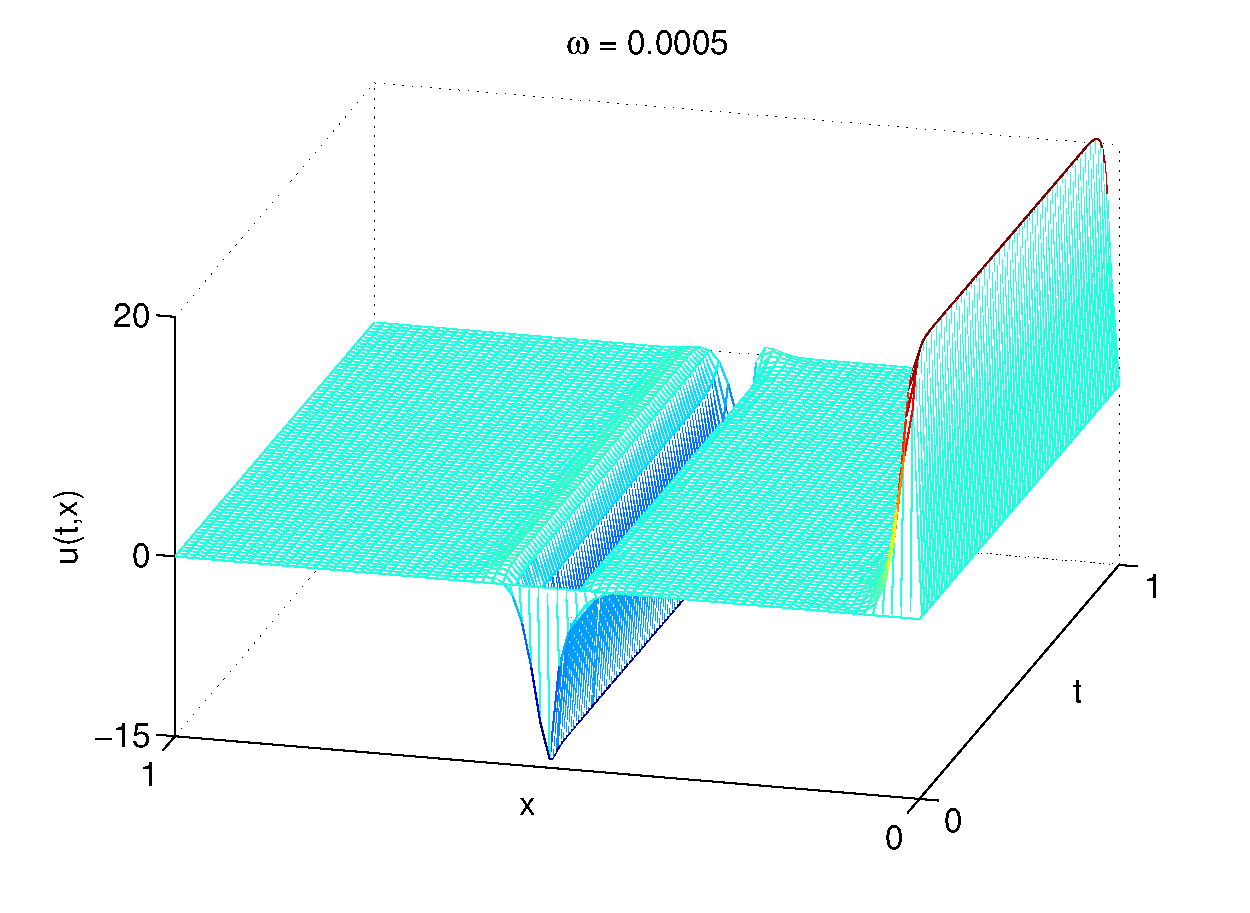
\includegraphics[width=0.33\textwidth]{plots/u_w0005}}\\
\caption{State $y$ and corresponding optimal control $u$ after convergence for different control parameters $\omega = \{0.05, 0.005, 0.0005\}$ .}\label{finalw}
\end{figure}
In Figure \ref{finalw} we see the final state of the optimization for different values of $\omega$ as well as the corresponding optimal control. For the smallest value of $\omega$, we see that the desired state is almost perfectly fitted and, therefore, the control has large values which leads to a large contribution in the cost function but has been compensated by the small value of $\omega$.
\subsection{Numerical results for gradient-based optimization methods}
\label{Num_SPG}
In this section, we present results corresponding to the BFGS and SPG methods as described in Section \ref{BFGS_section} and \ref{SPG_chap}, respectively. In our tests, we used publicly available \textsc{Matlab} implementations that require the cost function and the gradient as input as well as some tolerances and settings. With formula \eqref{minJ_discr} and Algorithm \ref{alg:Adj1_Burgers} we have already given a fully discretized version of the cost function and its gradient and, therefore, the application of both first-order optimization algorithms in straightforward. Here, we only present numerical results of the SPG method because this method allows us to impose bounds on the control $\mathbf{u}$ at all time instance. Accuracy and performance results for all approaches including the BFGS method are presented in Section \ref{numTests}. One can imagine that bounds on the control arise in many engineering application from physical constraints, cf. \cite{SCDA08}.

In Figure \ref{SPGu2}, we present the converged solution of the SPG method when the control is bounded between $-2$ and $2$. Clearly, this affects the corresponding optimal state of Burgers' solution and we can see that the desired state can not be reached with the same accuracy as in the previous examples.
\begin{figure}[H]
\centering
\includegraphics[width=0.8\textwidth]{plots/SPG_u2}
\caption{Optimal state (upper left), desired state (upper right), adjoint state (lower left) and optimal control (lower right) for a bounded control $-2 \leq u \leq 2$ using the SPG Algorithm \ref{alg:SPG}.}\label{SPGu2}
\end{figure}

\chapter{Implementation and analysis of a POD-DEIM reduced model for the optimal control of Burgers' equation}
\label{chap4}
In \cite{KV99}, the authors used a POD-reduced model for the optimal control of Burgers' equation. In this Section, we extend this approach by applying model order reduction using POD-DEIM as described in Section \ref{MOR_chap} to an optimal control problem as described in Section \ref{Opt_chap} and compare the POD-DEIM reduced model to the POD model in terms of computational cost and accuracy. The reduced optimal control problem is in the implicitly-constrained form,
\begin{equation}
\label{allgControl_small}
\begin{split}
\min_{u} \ &\tilde{\mathcal{J}}(\tilde{y}(u),u) ,\\
\text{with } \ &\tilde{c}(\tilde{y},u) = 0,
\end{split}
\end{equation}
where we use a tilde to indicate that the considered quantity is of lower dimension. In \eqref{allgControl_small}, the constraining nonlinear PDE $\tilde{c}(\tilde{y},u) = 0$ is solved for the reduced state variable $\tilde y(u)$. Since the evaluation of the cost function $\tilde{\mathcal{J}}$ requires the computation of $\tilde{y}$ first, this approach also leads to a faster evaluation of the cost function due to the lower dimension of the state variable. We will refer to the solution of \eqref{allgControl_small} as the optimal control of the reduced system. It is important to note, that even though this optimal control is derived from the reduced system, we denote it without tilde in order to stress that the control is still of the large dimension of the full-order model. This is a natural approach at this point because $u$ can be seen as an input variable because the state $\tilde{y}(u)$ directly depends on the control. A dimension reduction of the control $u$ is not considered at this point. Similarly to the previous section, we denote by $\hat{\tilde{\mathcal J}}(u) := \tilde{\mathcal{J}}(\tilde{y}(u),u)$ the cost function as a function of the control only.
\newpage
\section{A POD-DEIM reduced model for optimal control of Burgers' equation}
\label{redOptimalControl}
In Section \ref{fullOrderControl}, we introduced the optimal control problem \eqref{minJ}-\eqref{Burgers2}. We will now derive a POD-DEIM reduced model of the corresponding discrete optimization problem \eqref{minJ_discr}-\eqref{Burgers2_discr}. Therefore, we first consider the discretized objective function \eqref{minJ_discr} and recall that the reduced state variable has been derived in the following way,
\begin{align*}
\mathbf{y}(t) \approx \Phi_\ell \mathbf{\tilde y}(t),
\end{align*}
where the columns of the matrix $\Phi_\ell$ are the POD basis. When we plug in this approximation into \eqref{minJ_discr}, we obtain the reduced objective function,
\begin{align}
\label{redOpt}
\min_{\mathbf{u}_0,...,\mathbf{u}_{N_t}} \tilde{J}(\mathbf{\tilde y}_0,...,\mathbf{\tilde y}_{N_t},\mathbf{u}_0,...,\mathbf{u}_{N_t}) = \min_{\mathbf{u}_1,...,\mathbf{u}_{N_t}} \sum_{i=0}^{N_t} \delta \! t \left( \frac{1}{2} \mathbf{\tilde y}_i^T \mathbf{\tilde y}_i - \mathbf{\tilde z}^T\mathbf{\tilde y}_i + \frac{\omega}{2}\mathbf{u}_i^T M \mathbf{u}_i \right),
\end{align}
where the mass matrix in the first term vanishes due to the M-orthogonality of $\Phi_\ell$ and the reduced desired state $\mathbf{\tilde z}$ is given by,
\begin{align}
\label{zred}
\mathbf{\tilde z} &:= \Phi_\ell^T \mathbf{z} \in \mathbb{R}^\ell.
\end{align}
Note that \eqref{zred} can be pre-computed once the POD basis is obtained because the desired state of the full-order model is a given function, see \eqref{fullz}. We further note problem \eqref{redOpt} is still formulated in terms of the full-dimensional control $\mathbf{u}_i$ at the time instances $t_i$. In Section \ref{smallu_sec}, we will show one way in which a lower-dimensional control can lead to a reduced model that is completely independent of the full-order dimension $N$.

In order to obtain a POD-DEIM reduced model for the constraining Burgers' equation, we refer to Section \ref{fullOrderControl} and apply the POD-DEIM projection to \eqref{Burgers2_discr}. The fully discretized reduced constraint is, thus, given by
\begin{align}
\label{redBurgers}
\tilde{c}_i(\mathbf{\tilde y}_i,\mathbf{\tilde y}_{i+1},\mathbf{u}_{i+1}) \equiv \frac{1}{\delta \! t} \mathbf{\tilde y}_{i+1} - \frac{1}{\delta \! t}\mathbf{\tilde y}_i + \frac{1}{2} \tilde{B}(\tilde{F}\mathbf{\tilde y}_{i+1})^2 + \nu \tilde{C}\mathbf{\tilde y}_{i+1} - \mathbf{\tilde f} - \tilde{M} \mathbf{u}_{i+1} = 0,
\end{align}
where $i=0,...,N_t-1$ and a dimension reduction for the right-hand side as well as the projected mass matrix has been obtained,
\begin{align}
\label{fred}
\mathbf{\tilde f} &:= \Phi_\ell^T \mathbf{f} \in \mathbb{R}^\ell,\\
\label{M1red}
\tilde{M} &:= \Phi_\ell^T M \in \mathbb{R}^{\ell \times N}.
\end{align}
Note that $\tilde{M}$ still depends on $N$ and the matrices $\tilde{B}, \tilde{C}, \tilde{F}$ have been defined in \eqref{Bred}, \eqref{Cred}, \eqref{Fred}, respectively.

Furthermore, we note that the nonlinear term in \eqref{redBurgers} has to be considered as a function of the reduced variable $\mathbf{\tilde y}$ and has the slightly more complicated form,
\begin{align}
 \label{redNonlin}
 \tilde{\mathcal{N}}(\mathbf{\tilde{y}}_{i+1}) := \frac{1}{2} \tilde{B} (\tilde{F} \mathbf{\tilde{y}}_{i+1})^2.
\end{align}

The Lagrangian function of the reduced model can be obtained directly from \eqref{redOpt} and \eqref{redBurgers} and is given by,
\begin{align}
\label{redLag}
&\mathcal{\tilde L}(\mathbf{\tilde y}_0,...,\mathbf{\tilde y}_{N_t}, \mathbf{u}_0,...,\mathbf{u}_{N_t},\boldsymbol{\tilde \lambda}_1,...,\boldsymbol{\tilde \lambda}_{N_t}) \nonumber \\
&\ = \sum_{i=0}^{N_t} \delta \! t \left( \frac{1}{2} \mathbf{\tilde y}_i^T \mathbf{\tilde y}_i - \mathbf{\tilde z}^T\mathbf{\tilde y}_i + \frac{\omega}{2} \mathbf{u}_i^T M \mathbf{u}_i \right) \nonumber \\
&\quad +  \sum_{i=0}^{N_t-1} \boldsymbol{\tilde \lambda}_{i+1}^T \left( \frac{1}{\delta \! t} \mathbf{\tilde y}_{i+1} - \frac{1}{\delta \! t} \mathbf{\tilde y}_i + \frac{1}{2} \tilde{B} (\tilde{F} \mathbf{\tilde y}_{i+1})^2 + \nu \tilde{C} \mathbf{\tilde y}_{i+1} - \mathbf{\tilde f} - \tilde{M} \mathbf{u}_{i+1}  \right)
\end{align}
In \eqref{redLag}, we see that the adjoint variable $\boldsymbol{\tilde \lambda}_i \in \mathbb{R}^\ell$ is of the same dimension $\ell$ as the reduced state variable. This gives a good motivation for a faster solution of the adjoint equations \eqref{adjoint1} when applied to the POD-DEIM reduced model.
\section{A Newton-type method for the POD-DEIM reduced model}
\label{Newton_red_chapter}
In Section \ref{NumTests_Hess}, we have already seen that the application of the adjoints for derivative computation according to Algorithm \eqref{alg:Adj1} and \eqref{alg:Adj2} is straightforward but the derivation of partial derivatives of the nonlinear term is still involved when applied to a concrete problem. In Algorithm \ref{alg:Adj1_redBurgers}, we present the computation of the gradient of the reduced objective function which follows from the application of Algorithm \ref{alg:Adj1} to the reduced model \eqref{redOpt}-\eqref{redBurgers}.
\begin{algorithm}[H]
\caption{Algorithm \ref{alg:Adj1} applied to the reduced Burgers' model}
\label{alg:Adj1_redBurgers}
\begin{algorithmic}[1]
\STATE From the initial condition $\mathbf{\tilde y}_0$ and the current control $\mathbf{u}_0,...,\mathbf{u}_{N_t}$, solve the reduced Burgers' equation for $\mathbf{\tilde y}_1,...,\mathbf{\tilde y}_{N_t}$ according to \ref{redBurgers}
\STATE The adjoint equation \eqref{adjoint1} reads:
\begin{subequations}
\begin{align}
\label{AdjRedOrder_term}
\left(\frac{1}{\delta \! t}I_\ell + \tilde{\mathcal{N}}'(\mathbf{\tilde{y}}_{N_t})  +  \nu \tilde{C}\right)^T \boldsymbol{\tilde{\lambda}}_{N_t} &= -\delta \! t(\mathbf{\tilde{y}}_{N_t} - \mathbf{\tilde z} )\\
\label{AdjRedOrder}
\left(\frac{1}{\delta \! t}I_\ell + \tilde{\mathcal{N}}'(\mathbf{\tilde{y}}_{i})  + \nu \tilde{C}\right)^T \boldsymbol{\tilde{\lambda}}_i &= - (-\frac{1}{\delta \! t} I_\ell)^T \boldsymbol{\tilde{\lambda}}_{i+1} -\delta \! t( \mathbf{\tilde{y}}_{i} - \mathbf{\tilde z} ), \quad i = N_t-1,...,1
\end{align}
\end{subequations}
\STATE The gradient is computed according to formula \eqref{grad}:
\begin{align}
\label{gradRedOrder}
\nabla \hat{\tilde{\mathcal J}}(\mathbf{u}_0,...,\mathbf{u}_{N_t}) = \begin{pmatrix} \delta \! t \omega M \mathbf{u}_0 \\ \delta \! t \omega M \mathbf{u}_1 - \tilde{M}^T \boldsymbol{\tilde{\lambda}}_1 \\ \vdots \\ \delta \! t \omega M \mathbf{u}_{N_t} - \tilde{M}^T \boldsymbol{\tilde{\lambda}}_{N_t} \end{pmatrix}
\end{align}
\end{algorithmic}
\end{algorithm}
Because of the small dimension of the adjoint variable $\boldsymbol{\tilde{\lambda}}_i$, we note that the solution of the linear systems \eqref{AdjRedOrder_term}-\eqref{AdjRedOrder} can be obtained much faster than in the full-order case. In \eqref{AdjRedOrder_term} and \eqref{AdjRedOrder} and the remainder of the paper, $I_\ell$ denotes the identity matrix of dimensions $\ell \times \ell$. It is important to stress that the Jacobian of the nonlinearity \eqref{redNonlin} has to be computed in terms of the reduced variable $\mathbf{\tilde y}$ and is, hence, of dimension $\ell \times \ell$ as the the following computation shows:
\begin{align}
\label{Jac_non_red}
\tilde{\mathcal{N}}'(\mathbf{\tilde{y}}) = \frac{d}{d \mathbf{\tilde{y}}} \left( \frac{1}{2} \tilde{B} (\tilde{F}\mathbf{\tilde{y}})^2 \right) = \begin{pmatrix} \tilde{B}_{1,1} & \hdots & \tilde{B}_{1,m}\\ \vdots & & \vdots \\ \tilde{B}_{\ell,1} & \hdots & \tilde{B}_{\ell,m}  \end{pmatrix} \cdot \begin{pmatrix} \mathbf{\langle \tilde{y}} , \tilde{F}_1\rangle \tilde{F}_{1,1} & \hdots & \langle \mathbf{\tilde{y}} , \tilde{F}_1 \rangle \tilde{F}_{1,\ell} \\ \vdots & & \vdots \\ \langle \mathbf{\tilde{y}} , \tilde{F}_m \rangle \tilde{F}_{m,1} & \hdots & \langle \mathbf{\tilde{y}}. \tilde{F}_m \rangle \tilde{F}_{m,\ell}  \end{pmatrix}.
\end{align}
In \eqref{Jac_non_red}, we denoted by $\tilde{F}_i$ the $i$-th row of the matrix $\tilde{F}$ and $\tilde{B}_{i,j}, \tilde{F}_{i,j}$ denotes the entry of the respective matrix at position $i,j$. Here, $\langle \cdot , \cdot \rangle$ stands for the standard scalar product in $\mathbb{R}^\ell$. Note that because of the full dimension of $\mathbf{u}_i$, the gradient in \eqref{gradRedOrder} is still of dimension $N \cdot N_t \times 1$. Algorithm \ref{alg:Adj1_redBurgers} has also been used for the gradient computation that is required for the first-order optimization methods SPG and BFGS.

We next present the efficient computation of the Hessian-times-vector product $\nabla^2 \hat{\tilde{\mathcal J}} \cdot \mathbf{\underline{v}}$ using adjoints. Since the Hessian with respect to $u$ is of dimension $N \cdot N_t \times N \cdot N_t$, the corresponding vector used in Algorithm \ref{alg:Adj2_redBurgers} is of the following form, $\mathbf{\underline{v}} := (\mathbf{v}_0, ..., \mathbf{v}_{N_t})^T \in \mathbb{R}^{(N \cdot N_t) \times 1}$.
\begin{algorithm}[H]
\caption{Algorithm \ref{alg:Adj2} applied to the reduced Burgers' model}
\label{alg:Adj2_redBurgers}
\begin{algorithmic}[1]
\STATE We assume that we have already computed $\mathbf{\tilde{y}}_0,...,\mathbf{\tilde{y}}_{N_t}, \mathbf{u}_0,...,\mathbf{u}_{N_t},\boldsymbol{\tilde{\lambda}}_1,...,\boldsymbol{\tilde{\lambda}}_{N_t}$ in \mbox{Algorithm \ref{alg:Adj1_redBurgers}}
\STATE Equation \eqref{eqnw} reads:
\begin{subequations}
\begin{align}
\label{wRedOrder_init}
\mathbf{\tilde{w}}_0 &= 0 \\
\label{wRedOrder}
\left( \frac{1}{\delta \!t} I_\ell + \tilde{\mathcal{N}}'(\mathbf{\tilde{y}}_{i+1})  + \nu \tilde{C}\right) \mathbf{\tilde{w}}_{i+1} &=  - (-\frac{1}{\delta \! t}I_\ell)\mathbf{\tilde{w}}_i - \tilde{M}\mathbf{v}_{i+1} , \quad i = 0,...,N_t-1
\end{align}
\end{subequations}
\STATE Equation \eqref{eqnp} reads:
\begin{subequations}
\begin{align}
\label{pRedOrder_term}
\left( \frac{1}{\delta \!t} I_\ell + \tilde{\mathcal{N}}'(\mathbf{\tilde{y}}_{N_t})  + \nu \tilde{C} \right)^T \mathbf{\tilde{p}}_{N_t} &= \delta \! t I_\ell \mathbf{\tilde{w}}_{N_t} + \left( \tilde{\boldsymbol \lambda}_{N_t}^T \tilde{\mathcal{N}}(\mathbf{\tilde{y}}_{N_t}) \right)'' \mathbf{\tilde{w}}_{N_t} \\
\label{pRedOrder}
\left( \frac{1}{\delta \!t} I_\ell + \tilde{\mathcal{N}}'(\mathbf{\tilde{y}}_{i})  + \nu \tilde{C} \right)^T \mathbf{\tilde{p}}_{i} &=  -(-\frac{1}{\delta \! t}I_\ell)^T\mathbf{\tilde{p}}_{i+1} + \delta \! t I_\ell \mathbf{\tilde{w}}_i + \left( \tilde{\boldsymbol \lambda}_{i}^T \tilde{\mathcal{N}}(\mathbf{\tilde{y}}_{i}) \right)'' \mathbf{\tilde{w}}_{i}, \quad i = N_t-1,...,1
\end{align}
\end{subequations}
\STATE The Hessian times a vector $\mathbf{\underline{v}}$ is computed according to formula \eqref{hesseqn}:
\begin{align}
\label{HessRedOrder}
\nabla^2 \hat{\tilde{\mathcal{J}}}(\mathbf{u}_0,...,\mathbf{u}_{N_t}) \mathbf{\underline{v}} = \begin{pmatrix} \delta \! t \omega M \mathbf{v}_0 \\ -\tilde{M}^T \mathbf{\tilde{p}}_1 + \delta \! t \omega M \mathbf{v}_1\\ \vdots \\ -\tilde{M}^T \mathbf{\tilde{p}}_{N_t} + \delta \! t \omega M \mathbf{v}_{N_t} \end{pmatrix}
\end{align}
\end{algorithmic}
\end{algorithm}
\newpage
Note that the second partial derivative of the nonlinear term $\tilde{\boldsymbol \lambda}^T \tilde{\mathcal{N}}(\mathbf{\tilde{y}})$ with respect to the reduced variable $\mathbf{\tilde{y}}$ in step $3$ of the above algorithm is given by:
\begin{align*}
\frac{d^2}{d\mathbf{\tilde y}^2} \left( \tilde{\boldsymbol \lambda}^T \tilde{\mathcal{N}}(\mathbf{\tilde{y}}) \right) \mathbf{\tilde{w}} &=  \frac{d^2}{d\mathbf{\tilde y}^2} \left( \boldsymbol{\tilde{\lambda}}^T (\frac{1}{2} \tilde{B} (\tilde{F} \mathbf{\tilde{y}})^2) \right) \mathbf{\tilde{w}}
=\frac{d^2}{d\mathbf{\tilde y}^2} \left( \sum_{k=1}^\ell \lambda_k \frac{1}{2} \sum_{j=1}^m \tilde{B}_{k,j} \left( \sum_{i=1}^\ell \tilde{F}_{j,i}\tilde{y}_i \right)^2 \right) \mathbf{\tilde{w}} \\
&= \frac{d}{d\mathbf{\tilde y}} \begin{pmatrix} \sum_{k=1}^\ell \lambda_k \sum_{j=1}^m \tilde{B}_{k,j} \sum_{i=1}^\ell \tilde{F}_{j,i}\tilde{y}_i \cdot \tilde{F}_{j,1}\\ \vdots \\ \sum_{k=1}^\ell \lambda_k \sum_{j=1}^m \tilde{B}_{k,j} \sum_{i=1}^\ell \tilde{F}_{j,i}\tilde{y}_i \cdot \tilde{F}_{j,\ell} \end{pmatrix}\mathbf{\tilde{w}} \\
&= \underbrace{\begin{pmatrix} \sum_{k=1}^\ell \lambda_k \sum_{j=1}^m \tilde{B}_{k,j} \tilde{F}_{j,1} \tilde{F}_{j,1} & \hdots & \sum_{k=1}^\ell \lambda_k \sum_{j=1}^m \tilde{B}_{k,j} \tilde{F}_{j,\ell} \tilde{F}_{j,1}\\ \vdots & & \vdots \\ \sum_{k=1}^\ell \lambda_k \sum_{j=1}^m \tilde{B}_{k,j} \tilde{F}_{j,1} \tilde{F}_{j,\ell} & \hdots & \sum_{k=1}^\ell \lambda_k \sum_{j=1}^m \tilde{B}_{k,j} \tilde{F}_{j,\ell} \tilde{F}_{j,\ell} \end{pmatrix}}_{\in \mathbb{R}^{\ell \times \ell}} \mathbf{\tilde{w}}
\end{align*}
Due to the dimensions of the reduced variables, it is natural that the above matrix-times-vector product only depends on the dimension $\ell$. The matrix is not constant in time because the adjoint variable depends on time and can, thus, not be pre-computed. An efficient implementation is therefore necessary in order to obtain a computational speedup if $\ell \ll N$.

Algorithm \ref{alg:Opt+MOR1} gives an overview of the optimization algorithm that has been developed for the optimal control of the POD-DEIM reduced model of Burgers' equation. Algorithm \ref{alg:Opt+MOR1} is an iterative procedure to update the reduced model aiming to improve the approximation to the full-order model. The procedure is as follows: In order to obtain snapshots, it is necessary to solve the full-order model corresponding to an initial control once. From snapshots of the full-order solution, we can derive the reduced model and solve the \textit{reduced} optimization problem for an optimal control. The reduced model can be improved in an iterative process by obtaining new snapshots of the state corresponding to the current optimal control. Then, a new POD-DEIM model is derived from the new snapshots and the same optimization algorithm is applied to the improved reduced model. This can be repeated until a certain stopping criterion is satisfied. In Algorithm \ref{alg:Opt+MOR1}, we improve the reduced model as long as the obtained optimal state is close enough to the desired state $z$ measured in the $L_2$-norm. Another approach for stopping could be that the reduced objective function reaches the value of the objective function of the full-order model evaluated at the optimal state. This, however, is only possible if the full-order optimal control has already been solved which we want to avoid in our implementation.
\newpage
\begin{algorithm}[H]
\caption{Optimal control: Iterative improvement of the reduced model}
\label{alg:Opt+MOR1}
\begin{algorithmic}[1]
\STATE Set initial control $u^{(0)} = 0$, and $K = 0$, $\varepsilon_z \in \mathbb{R}_+$, \texttt{max\_iter} $\in \mathbb{N}$
\STATE Solve the full-order Burgers' equation $c(y^{(0)},u^{(0)})$ for the uncontrolled state $y^{(0)}$ via \eqref{Burgers2_discr}
\STATE Choose POD dimension $\ell$ and DEIM-dimension $m$
\WHILE{$\|y^{(K)}-z\|_{L^2([0,L] \times [0,T])} > \varepsilon_z$ \AND $K < $\texttt{max\_iter}}
\STATE Obtain the POD-DEIM reduced model from snapshots of $y^{(K)}$, i.e. compute $\Phi_\ell$ via \eqref{Phidef} and $\mathcal{P}$ via Algorithm \ref{alg:DEIM}
\STATE Calculate reduced optimal control, $u^{(K+1)} = \argmin_u \tilde{\mathcal J}(\tilde{y}(u),u)$ by solving the reduced optimization problem \eqref{redOpt} with implicit constraint \eqref{redBurgers}. Choose one of the optimization algorithms \ref{alg:Opt}, \ref{alg:BFGS} or \ref{alg:SPG}.
\STATE Solve the reduced Burgers' equation $\tilde{c}(\tilde{y}^{(K+1)},u^{(K+1)}) = 0$ for $\tilde{y}^{(K+1)}$ via \eqref{redBurgers}
\STATE Expand $y^{(K+1)} = \Phi_\ell \tilde{y}^{(K+1)}$
\STATE $K = K + 1$
\ENDWHILE
\end{algorithmic}
\end{algorithm}
In Figure \ref{optred}, we show numerical results for the optimal control of Burgers' equation using a POD-DEIM reduced model of different dimensions $\ell$ and $m$ and using the Newton-type method of Algorithm \ref{alg:Opt} for solving the optimization problem. We see that due to the low-dimensional state variable, the desired state is not reached with the same accuracy as in the full-order case. This leads to a larger optimal value of the objective function \eqref{redOpt} as the results in Section \ref{numTests} will show.
\begin{figure}[H]
\centering
\subfloat[$\ell = m = 7$]{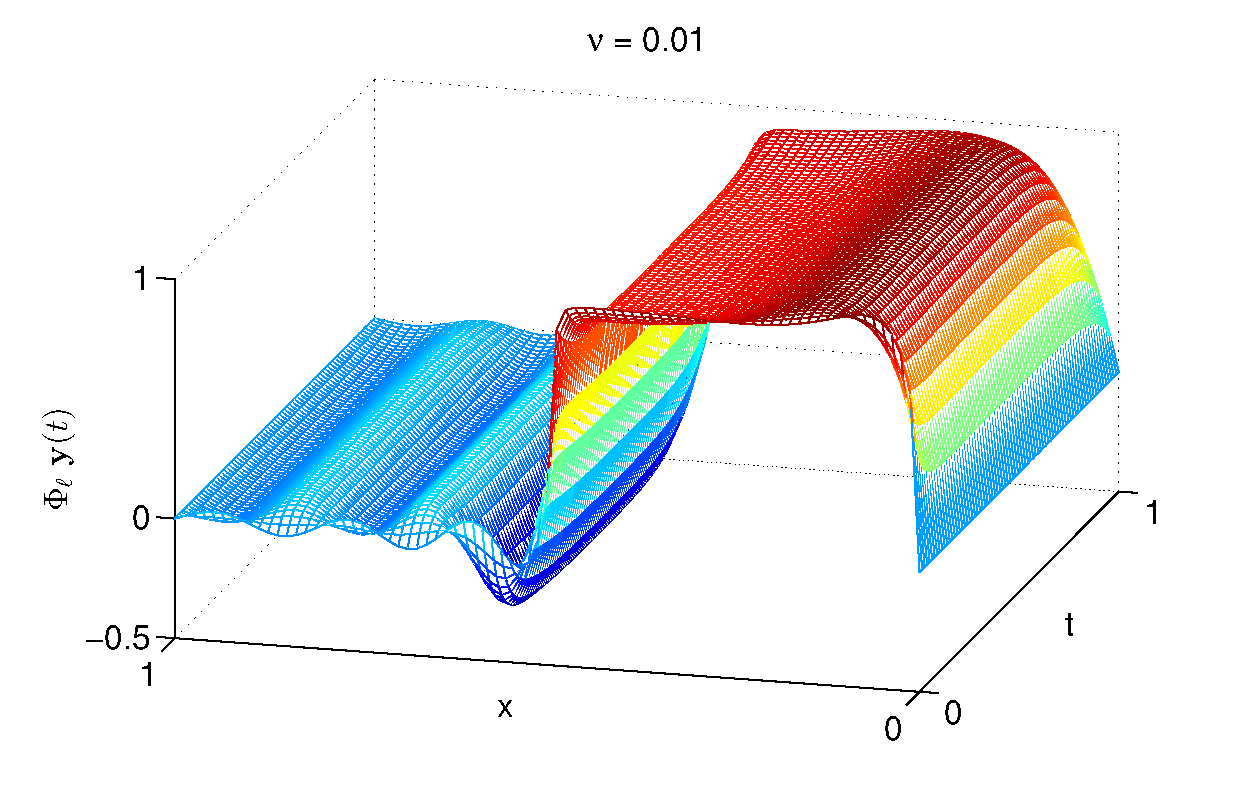
\includegraphics[width=0.49\textwidth]{plots/redOptCon_y7}}\hfill
\subfloat[$\ell = m = 15$]{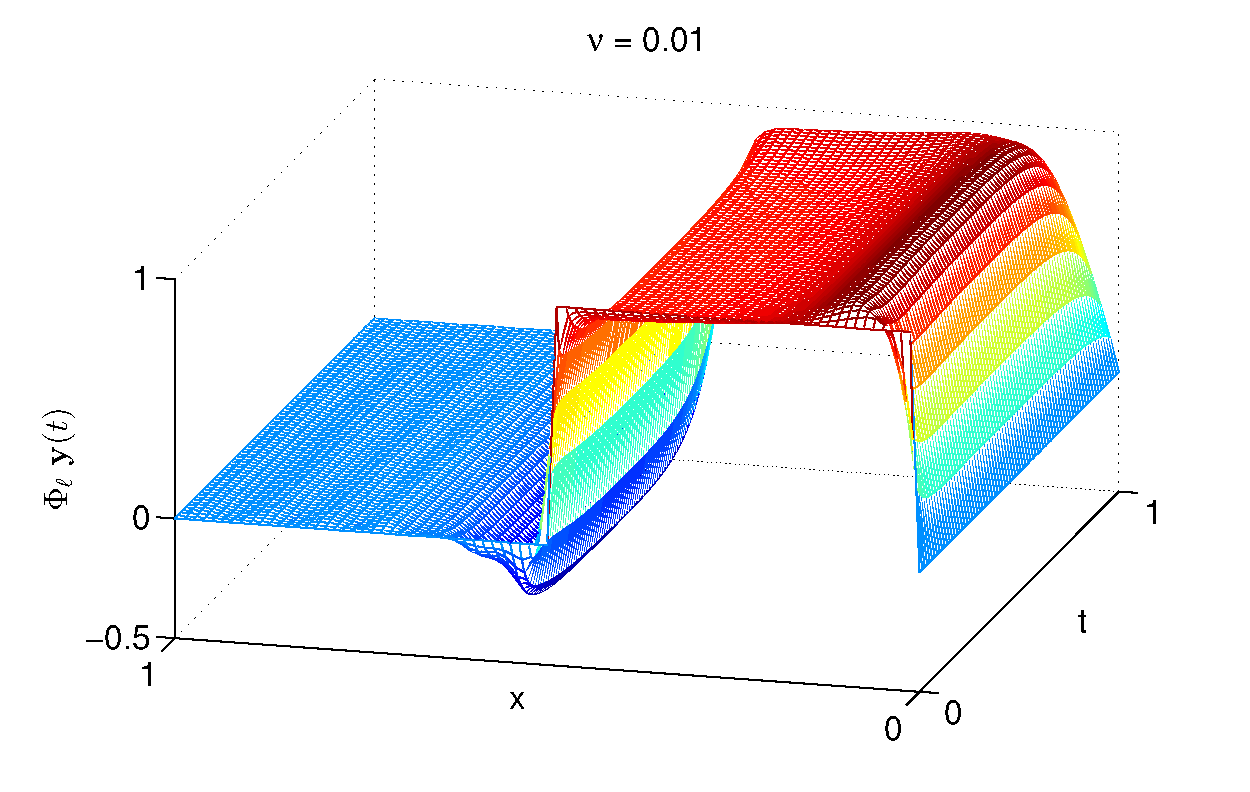
\includegraphics[width=0.49\textwidth]{plots/redOptCon_y15}}\\
\subfloat[$\ell = m = 7$ ]{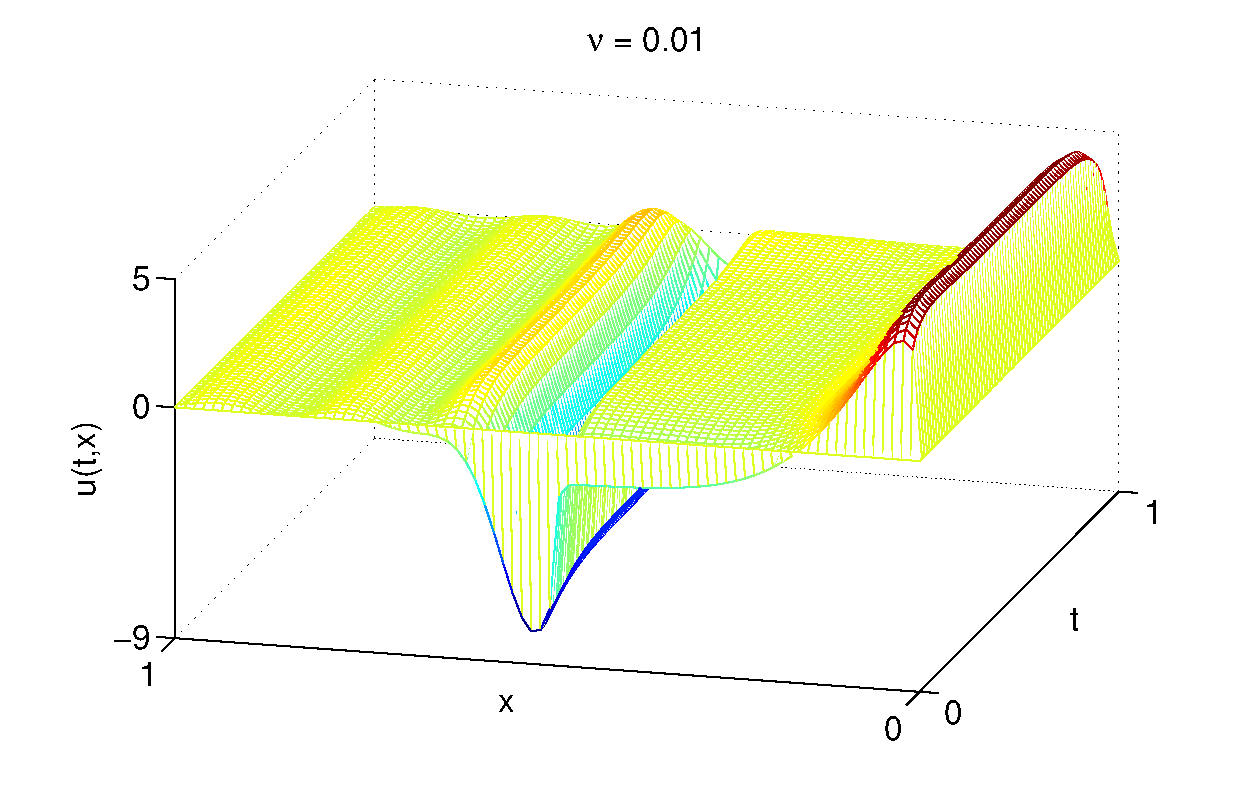
\includegraphics[width=0.49\textwidth]{plots/redOptCon_u7}}\hfill
\subfloat[$\ell = m = 15$]{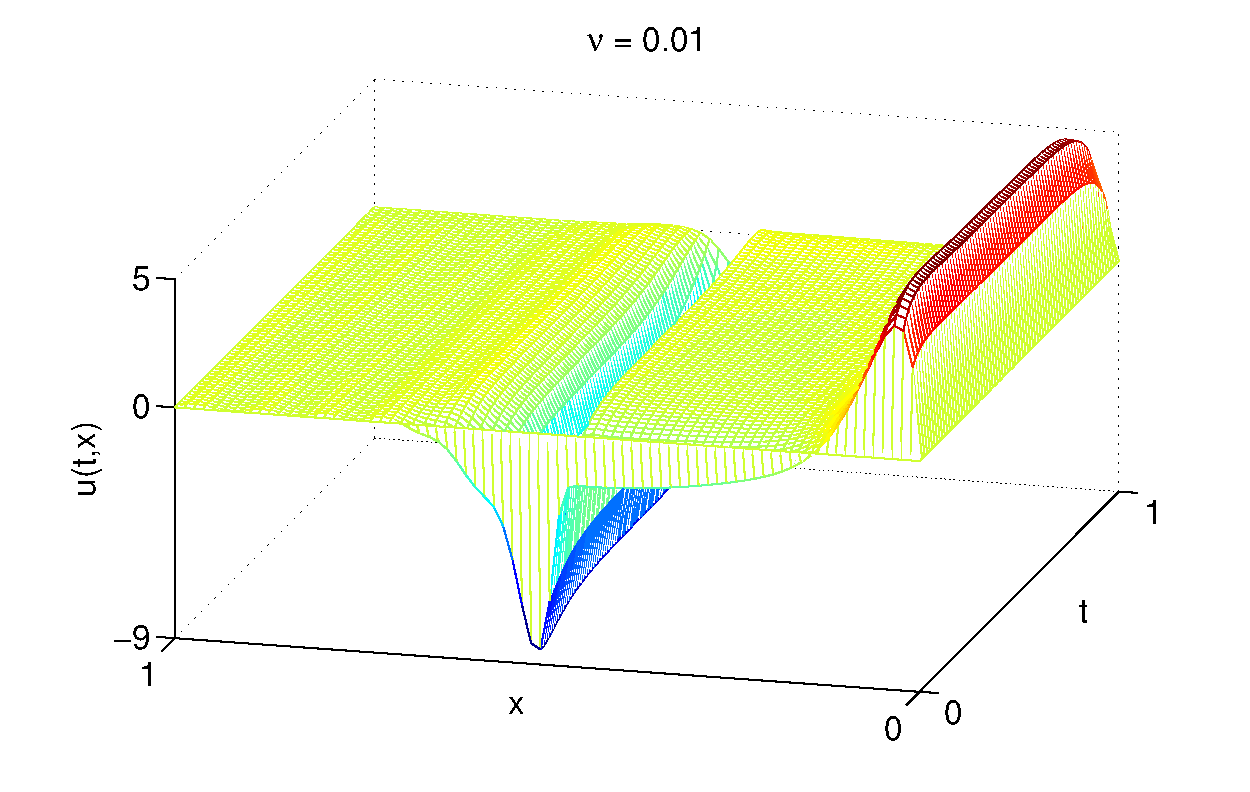
\includegraphics[width=0.49\textwidth]{plots/redOptCon_u15}}\\
\caption{Optimal control of the POD-DEIM reduced Burgers' model using different dimensions.}\label{optred}
\end{figure}
%\begin{algorithm}[H]
%\caption{Optimal control: Improving the reduced model using the full-order system}
%\label{alg:Opt+MOR}
%\begin{algorithmic}[1]
%\STATE Set initial control $\mathbf{\underline{u}}^{(0)} = 0$, and $k = 0$, $tol \in \mathbb{R}_+$, \texttt{MAX\_FULL} $\in %\mathbb{N}$
%\STATE Solve the full-order Burgers' equation \eqref{Burgers2_discr} for $\mathbf{\underline{y}}^{(0)}$ (uncontrolled %state)
%\WHILE{$k <$ \texttt{MAX\_FULL}}
%\STATE Set $\mathbf{\underline{u}}_{\text{old}} = \mathbf{\underline{u}}^{(k)}$
%\STATE Obtain the POD-DEIM reduced model from snapshots of $\mathbf{\underline{y}}^{(k)}$ and %$\mathbf{\underline{u}}^{(k)}$, i.e compute $\Phi_\ell$ via \eqref{Phidef}, $\Psi_\ell$ via \eqref{Psidef} and %$\mathcal{P}$ via Algorithm \ref{alg:DEIM}
%\STATE Calculate reduced control $\mathbf{\underline{\tilde u}}^{(k+1)}$ by solving the reduced optimization problem %\eqref{redOpt} subject to \eqref{redBurgers} via Algorithm \ref{alg:Opt}
%\STATE Set $\mathbf{\underline{u}}_{\text{new}} = \text{blkdiag}(\Psi_\ell)\mathbf{\underline{\tilde u}}^{(k+1)}$
%\IF{$\|\mathbf{\underline{u}}_{\text{old}} - \mathbf{\underline{u}}_{\text{new}}\| < tol$}
%\RETURN
%\ELSE
%\STATE Calculate full-order control $\mathbf{\underline{u}}^{(k+1)}$ by solving the optimization problem \eqref{minJ_discr} %subject to \eqref{Burgers2_discr} via Algorithm \ref{alg:Opt}
%\ENDIF
%\STATE $k = k + 1$
%\ENDWHILE
%\end{algorithmic}
%\end{algorithm}

%\begin{figure}[H]
%\centering
%\subfloat[$k=1$ (uncontrolled)]{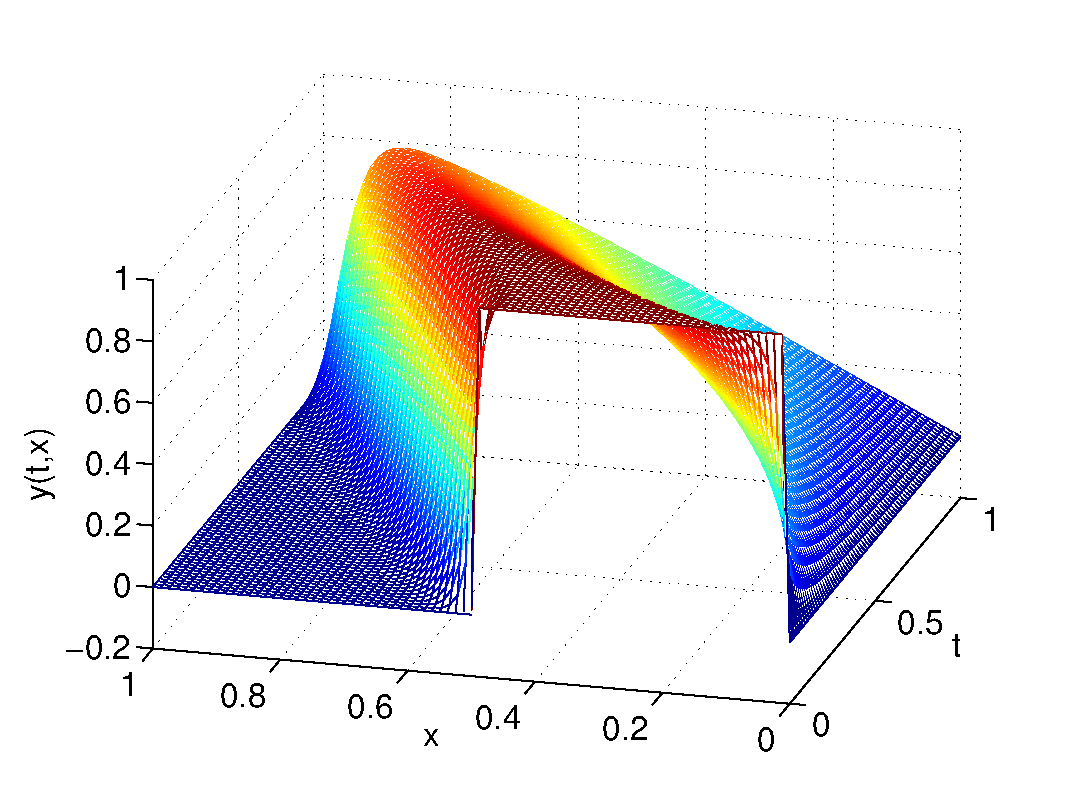
\includegraphics[width=0.49\textwidth]{plots/controlRedk1}}\hfill
%\subfloat[$k=2$]{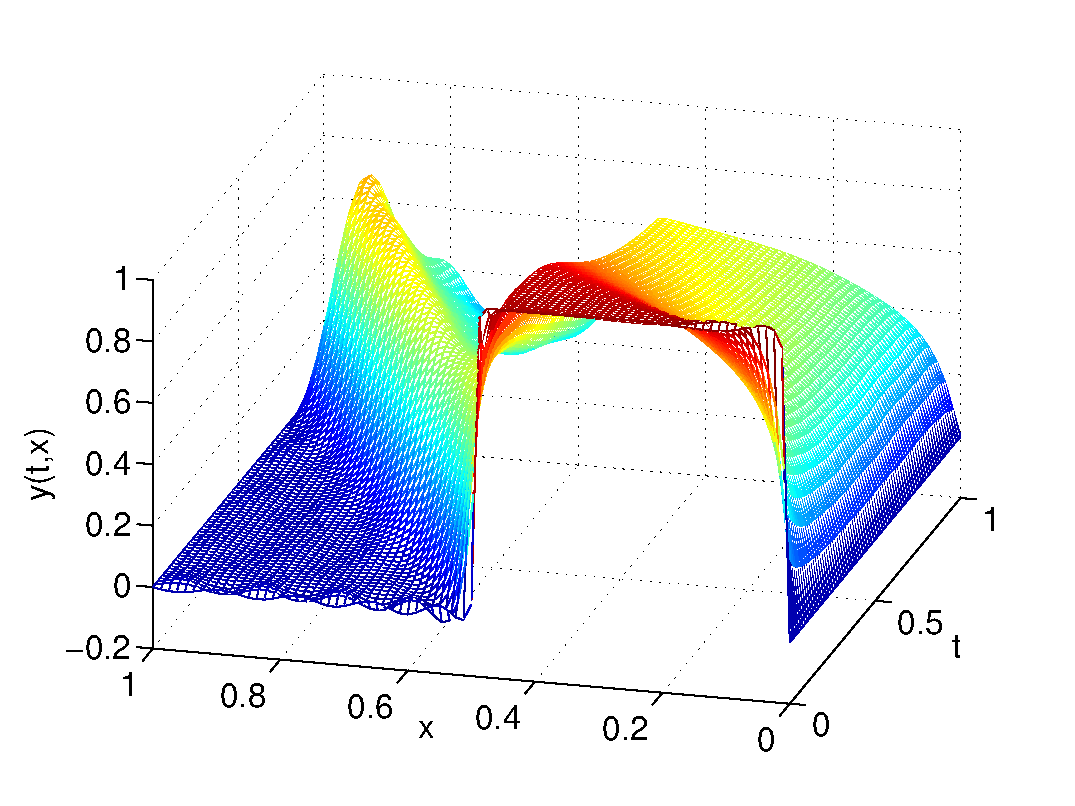
\includegraphics[width=0.49\textwidth]{plots/controlRedk2}}\\
%\subfloat[$k=5$ ]{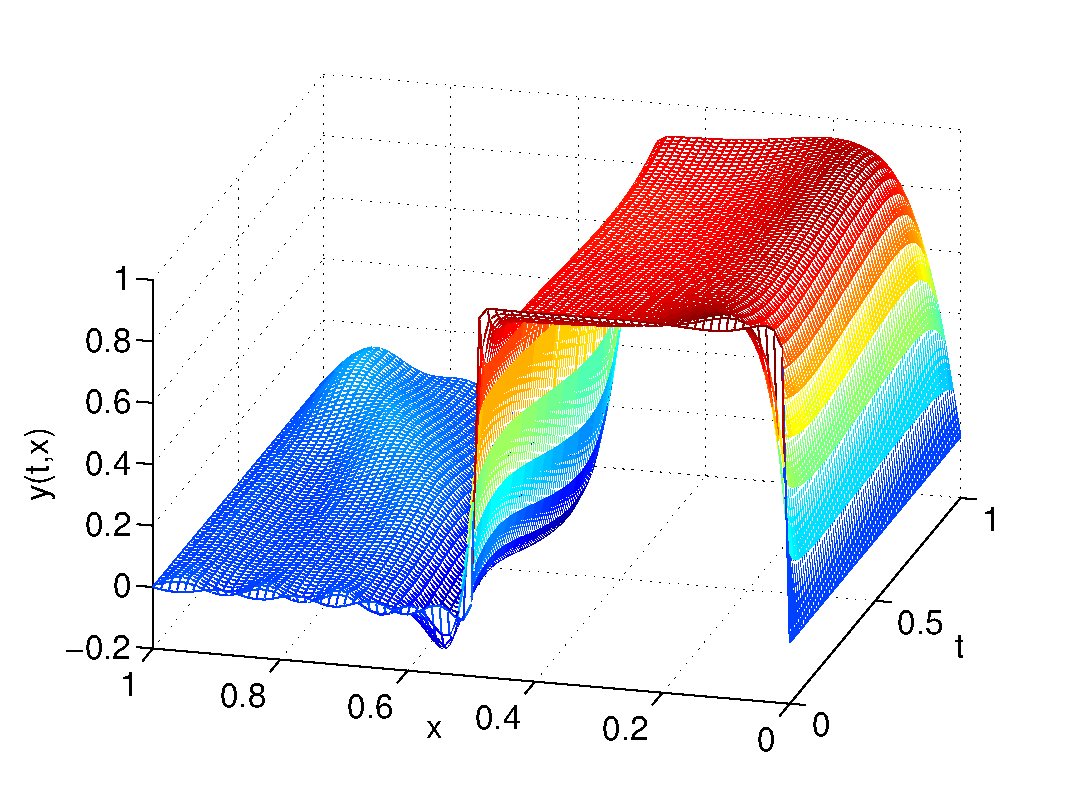
\includegraphics[width=0.49\textwidth]{plots/controlRedk5}}\hfill
%\subfloat[$k=10$]{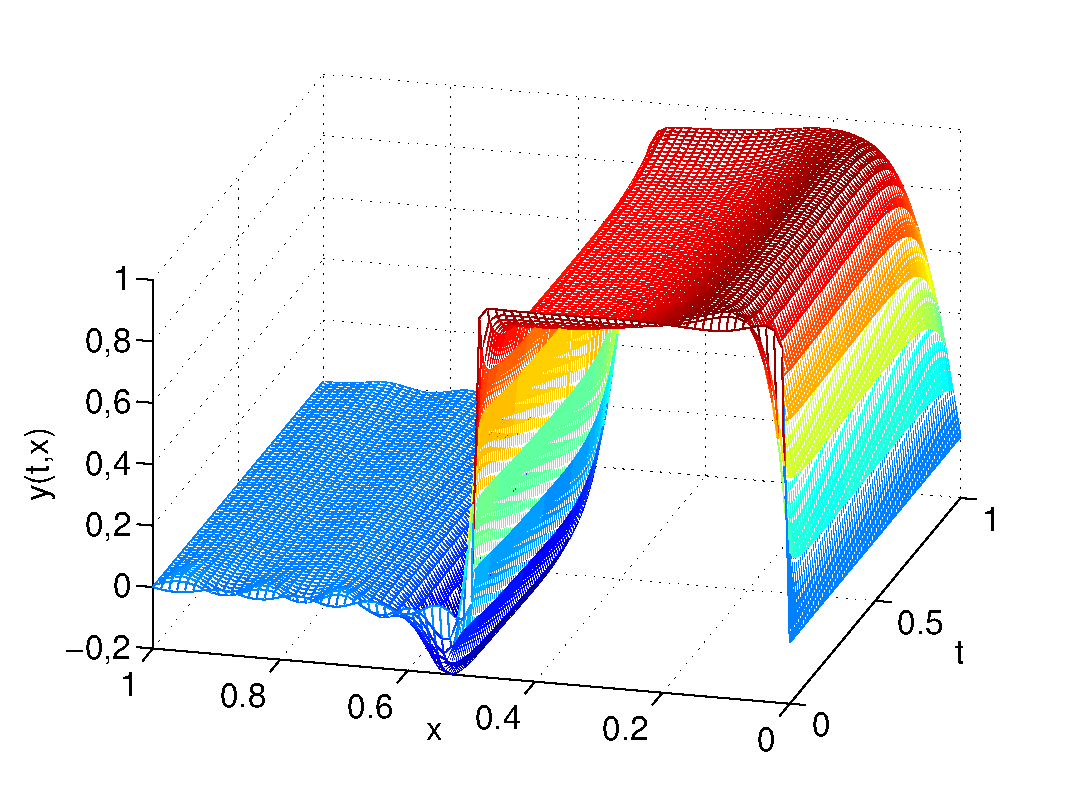
\includegraphics[width=0.49\textwidth]{plots/controlRedk10}}\\
%\caption{Reduced-order optimization.}\label{optRed}
%\end{figure}

%\begin{figure}[H]
%\centering
%\subfloat[$k=1$ (initial)]{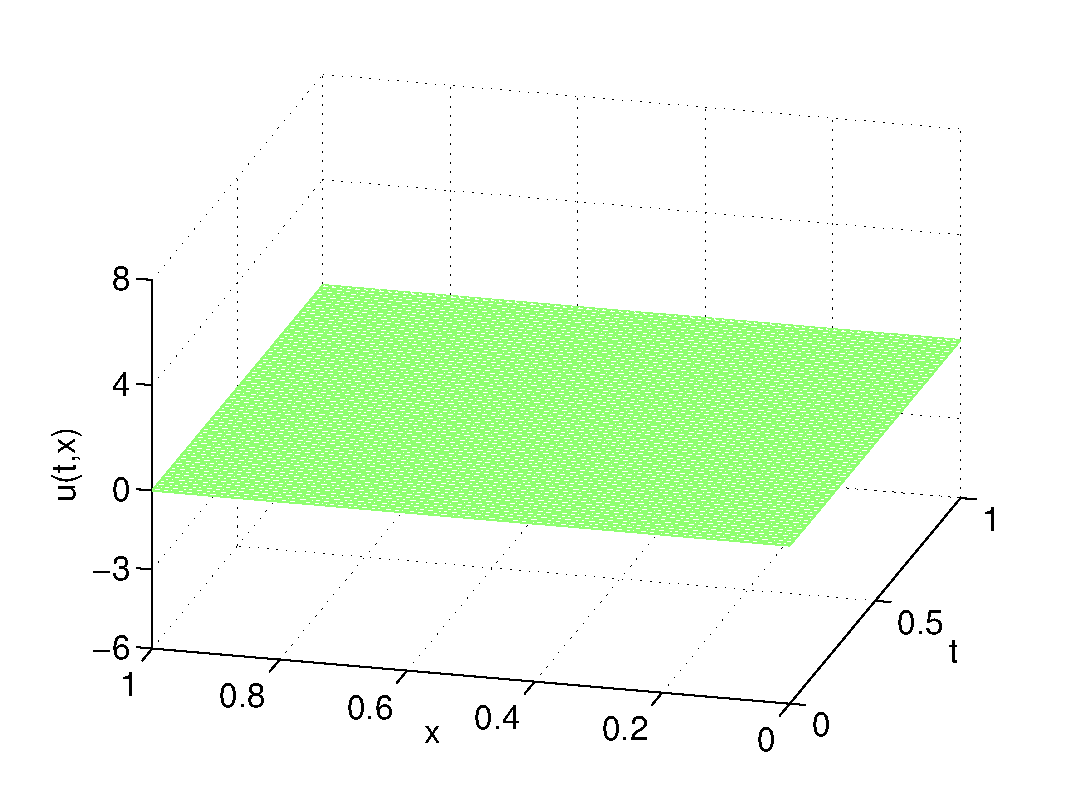
\includegraphics[width=0.49\textwidth]{plots/uRedk1}}\hfill
%\subfloat[$k=2$]{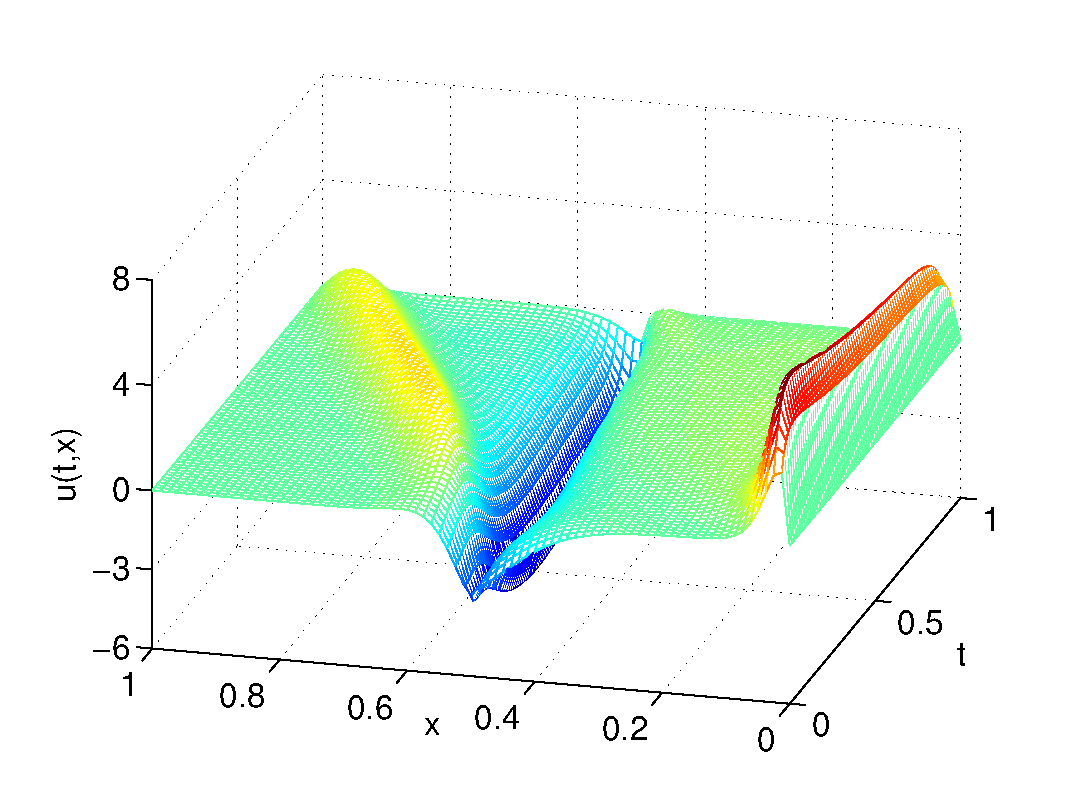
\includegraphics[width=0.49\textwidth]{plots/uRedk2}}\\
%\subfloat[$k=5$ ]{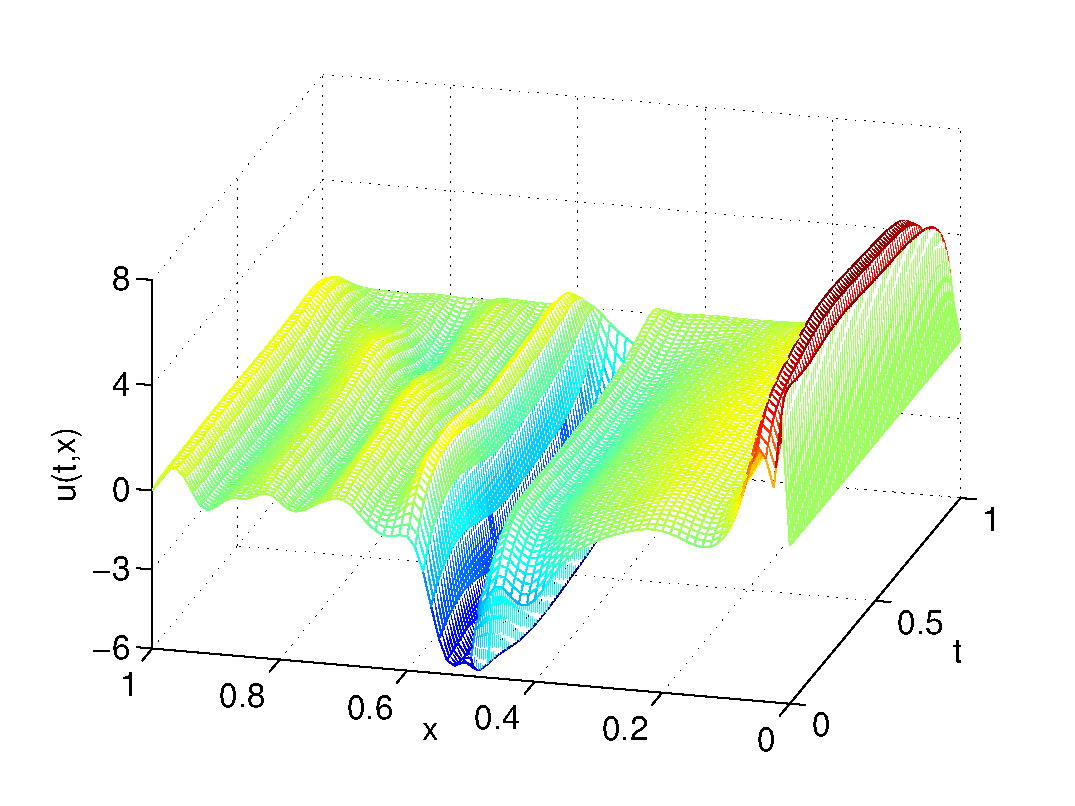
\includegraphics[width=0.49\textwidth]{plots/uRedk5}}\hfill
%\subfloat[$k=10$]{\includegraphics[width=0.49\textwidth]{plots/uRedk10}}\\
%\caption{Reduced-order control.}\label{optRedu}
%\end{figure}
\section{Low-dimensional control using individual control points}
\label{smallu_sec}
In order to overcome the dependence of the control on the dimension of the full-order model, we will restrict the control to certain discrete \textit{control points}. In Figure \ref{smallu}, we have indicated that we allow to control the system at only three different points in $[0,L]$. This approach requires, of course, some physical inside of the problem in the sense that we need to know at which points it is important to control the state.
\begin{figure}[H]
\centering
\includegraphics[width=0.49\textwidth]{plots/smallu.png}
\caption{Discretization of the interval $[0,L]$ indicating only $3$ discrete positions for control.}\label{smallu}
\end{figure}
We can model this approach by writing the control in the following way:
\begin{align}
\label{lowDimu}
\mathbf{u}(t) = \Psi_{n_c} \mathbf{\tilde u}(t), \quad \text{with } \mathbf{\tilde u}(t) \in \mathbb{R}^{n_c},
\end{align}
where $\mathbf{\tilde u}(t)$ is low-dimensional and contains only non-zero values of the control at the $n_c$ considered points. The matrix $\Psi$ indicates which entries of the control we want to consider. For the case in Figure \ref{smallu} with $n_c  = 3$, we would have:
\begin{align*}
\Psi_3 = \begin{pmatrix} 1 & 0 & 0 \\
                           &   \vdots & \\
                         0 & 1 & 0  \\
                         0 & 0 & 1  \\
                           &  \vdots &  \end{pmatrix} \in \mathbb{R}^{N \times 3}.
\end{align*}
Note that this decomposition corresponds to an ansatz:
\begin{align*}
u(t,x) \approx \sum_{j \in \mathcal{I}_{c}} u_j(t) \phi_j(x),
\end{align*}
with an index set $\mathcal{I}_{c}$ containing $n_c$ indices of the control points. This way, the mass matrix for the control can be derived in a straightforward way but the approach of \eqref{lowDimu} shows the gain in dimension reduction better: When we plug in \eqref{lowDimu} into the discretized objective function \eqref{redOpt}, we obtain:
\begin{align}
\label{redOpt_smallu}
\min_{\mathbf{\tilde{u}}_0,...,\mathbf{\tilde{u}}_{N_t}} \tilde{J}(\mathbf{\tilde y}_0,...,\mathbf{\tilde y}_{N_t},\mathbf{\tilde{u}}_0,...,\mathbf{\tilde{u}}_{N_t}) = \min_{\mathbf{\tilde{u}}_1,...,\mathbf{\tilde{u}}_{N_t}} \sum_{i=0}^{N_t} \delta \! t \left( \frac{1}{2} \mathbf{\tilde y}_i^T \mathbf{\tilde y}_i - \mathbf{\tilde z}^T\mathbf{\tilde y}_i + \frac{\omega}{2}\mathbf{\tilde{u}}_i^T \underbrace{\Psi^T M \Psi}_{\text{pre-compute}} \mathbf{\tilde{u}}_i \right),
\end{align}
which does not depend on the full-order dimension $N$ at all because the matrix $\Psi^T M \Psi \in \mathbb{R}^{n_c \times n_c}$. Note also that this matrix can be pre-computed. In the same way, we have for the discretized reduced Burgers' equation \eqref{redBurgers} the following:
\begin{align}
\label{redBurgers_smallu}
\tilde{c}_i(\mathbf{\tilde y}_i,\mathbf{\tilde y}_{i+1},\mathbf{\tilde u}_{i+1}) \equiv \frac{1}{\delta \! t} \mathbf{\tilde y}_{i+1} - \frac{1}{\delta \! t}\mathbf{\tilde y}_i + \frac{1}{2} \tilde{B}(\tilde{F}\mathbf{\tilde y}_{i+1})^2 + \nu \tilde{C}\mathbf{\tilde y}_{i+1} - \mathbf{\tilde f} - \underbrace{\Phi_\ell^T M \Psi}_{\text{pre-compute}} \mathbf{\tilde u}_{i+1} = 0,
\end{align}
where $i=0,...,N_t-1$ and $\Phi_\ell^T M \Psi \in \mathbb{R}^{\ell \times n_c}$.

In Figure \ref{result_Smallu}, we show the numerical result for $n_c = 3$. We see that even a control at only three different control points leads to a reasonable approximation to the desired state. We also present the corresponding control that drives the solution to the POD-DEIM reduced Burgers' equation into the desired state.
\begin{figure}[H]
\centering
\includegraphics[width=0.49\textwidth]{plots/y_smallu} \hfill
\includegraphics[width=0.49\textwidth]{plots/u_smallu}
\caption{Optimal control (right) and corresponding state (left) for $\ell = m = 11$ and $n_c = 3$ control points.}\label{result_Smallu}
\end{figure}
\section{Performance and error analysis}
\label{numTests}
The main goal of this thesis work is to evaluate the performance of POD-DEIM when applied to optimal control of Burgers' equation. In order to compare the results of the optimization using a POD-DEIM reduced model with the optimization based on a reduced model obtained from a pure POD reduction as suggested in \cite{KV99}, it is important to specify identical stopping criteria and tolerances for the respective numerical optimization algorithm. In this section, we present numerical results for three different viscosity parameters, $\nu = \{0.01, 0.001, 0.0001\}$, and for the three different optimization algorithms Newton-type, BFGS and SPG as presented in Section \ref{optAdj}, \ref{BFGS_section} and \ref{SPG_chap}, respectively. Since all three optimization algorithms are iterative methods, we are able to define a stopping of the optimization when either the change in the objective function is smaller than the tolerance $\varepsilon_\mathcal{J}$ or the zero-gradient condition is fulfilled upto a numeric tolerance specified by $\varepsilon_\nabla$. For the presented results of this section, we used  $\varepsilon_\mathcal{J} =$ \texttt{10e-8} and $\varepsilon_\nabla =$ \texttt{10e-9} in the respective Algorithms \ref{alg:Opt}, \ref{alg:BFGS} or \ref{alg:SPG}. In general, it is difficult to design a \textit{fair} comparison between different algorithms. For example, the stopping criterion for the gradient is implemented differently for the SPG method, see line $5$ of Algorithm \ref{alg:SPG}. Therefore, we also used a criterion which is called \textit{targeting} and which provides comparable results by choosing all parameters in such a way that the final value of the reduced objective function and the objective function of the full-order model are close. Moreover, we have required the error of the optimal state in the relative $L_2$-norm to be small.

In order to compare the optimal control of the POD and the POD-DEIM reduced Burgers' model, we are first interested in the \textit{accuracy} of the optimal state obtained by the two reduced models in comparison to the full-order optimal control as described in Section \ref{fullOrderControl}. Therefore, we choose the viscosity parameter $\nu = 0.01$ which requires a dimension of $N = 80$ for the full-order model, cf. Section \ref{fullOrderControl}. For a comparison of the optimal state obtained by a POD and POD-DEIM, we choose the DEIM-dimension constant, $m = 15$, and increase the POD dimension $\ell$ from $3$ to $25$. In Figure \ref{YerrL2}, we present the distribution of the error which is defined as the squared difference of the final state of the full-order optimization and the final state of the respective optimization of the reduced model,
\begin{align*}
 e(t,x) := [y(t,x) - \Phi_\ell \tilde{y}(t)]^2.
\end{align*}
Figure \ref{YerrL2} shows the error as a function of time and space for three different POD dimensions, $\ell = \{5,15,25\}$. We see that the error is large where the desired state is not smooth, i.e. at the boundary of the step function $z$. Furthermore, the plot in Figure \ref{YerrL2} shows that the error decreases as the POD dimension increases. For all three cases considered, the error is generally larger for the POD-DEIM reduced model but it is always of the same order of magnitude.
\begin{figure}[H]
\centering
\subfloat[$\ell = 5$]{\includegraphics[width=0.33\textwidth]{plots/YerrL2_pod_5_new}}\hfill
\subfloat[$\ell = 15$]{\includegraphics[width=0.33\textwidth]{plots/YerrL2_pod_15_new}}\hfill
\subfloat[$\ell = 25$]{\includegraphics[width=0.33\textwidth]{plots/YerrL2_pod_25_new}}\hfill \\
\subfloat[$\ell = 5$]{\includegraphics[width=0.33\textwidth]{plots/YerrL2_poddeim_5_new}}\hfill
\subfloat[$\ell = 15$]{\includegraphics[width=0.33\textwidth]{plots/YerrL2_poddeim_15_new}}\hfill
\subfloat[$\ell = 25$]{\includegraphics[width=0.33\textwidth]{plots/YerrL2_poddeim_25_new}}\hfill \\
\caption{Error distribution of the optimal state obtained by the Newton-type method and a POD and POD-DEIM reduced model.}\label{YerrL2}
\end{figure}
\newpage
In Figure \ref{L2err}, we present the error in the two reduced optimal sates with respect to the full optimal state not as a function of time and space but calculated in the corresponding $L_2$-norm. Since the POD reduced model only depends on $\ell$, we have again chosen a fixed DEIM-dimension $m = 15$ in order to compare the error in $L_2$ as a function of $\ell$. In Figure \ref{L2err}, we see that, as expected, the POD-DEIM error is larger for all considered $\ell$. It is also interesting to note that for $\ell > m$, the error of the POD-DEIM optimal state is dominated by the DEIM approximation error and does not decrease further whereas the error of the optimal state obtained from the POD reduced model still decreases.
\begin{figure}[H]
\centering
\includegraphics[width=0.66\textwidth]{plots/yL2err}
%\subfloat{\includegraphics[width=0.7\textwidth]{plots/uL2err}}
\caption{Comparison of the $L_2$-error of the POD and the POD-DEIM approximation when the projection dimensions are increased.}\label{L2err}
\end{figure}
The results presented in Figure \ref{YerrL2} and Figure \ref{L2err} show that the POD-DEIM reduced optimal control problem \eqref{redOpt}-\eqref{redBurgers} yields to a comparable optimal solution to a POD-reduced model and the full-order optimal control problem \eqref{minJ_discr}-\eqref{Burgers2_discr}. We will next consider the application of the Newton-type optimization method of Algorithm \ref{alg:Opt} to the three different models with respect to computational time. Therefore, we have calculated the optimal solution for three different values of $\nu$ in Table \ref{time_messure1}. The measurements reported in Table \ref{time_messure1} are:
\begin{itemize}
 \item $N$/$\ell$/$m$ - The (spatial) dimension of the full-order, POD and POD-DEIM reduced model, respectively. In the case of POD-DEIM we present both reduced dimensions as the tuple $(\ell,m)$
 \item $t_{opt}[s]$ - This is the time needed for the considered optimization algorithm. In case of the reduced optimal control presented in Algorithm \ref{alg:Opt+MOR1}, this also includes the time which is necessary for building the reduced model, i.e. the pre-computation of the POD basis and DEIM-indices.
 \item $\mathcal{J}(y^*,u^*)$ - The value of the (reduced) objective function after convergence of the optimization iteration.
 \item $\bar{e}$ - The relative error as defined in \eqref{relErr_def}, computed for the optimal state.
 \item $S_P$ - The speedup in computation time.
\end{itemize}
\newpage
\begin{table}[H]
\centering
\begin{tabular}{|c|c|c|c|c|c|c|c|c|c|}
\cline{1-10}
 & \multicolumn{3}{ c| }{$\nu = 0.01$} & \multicolumn{3}{ c| }{$\nu = 0.001$}& \multicolumn{3}{ c| }{$\nu = 0.0001$}\\ \cline{2-10}
 & Full & POD & DEIM & Full & POD & DEIM & Full & POD & DEIM \\ \cline{1-10}
$N$/$\ell$/$m$ & $80$ &$ 9 $&$(9,25)$ &$200$ &$11$ &$(11,25)$ & $800$&$15$ & $(15,25)$\\ \cline{1-10}
$t_{opt}[s]$        & 4.83      &4.13      &3.22       & 23.1 & 6.38 & 5.25 & 1,865.8 & 23.61 & 18.42 \\ \cline{1-10}
$\mathcal{J}(y^*,u^*)$   &  0.0241      & 0.0262      &0.0233        & 0.0206 & 0.0198 & 0.0200 &0.0202 & 0.0191 &0.0233 \\ \cline{1-10}
$\bar{e}$ &- & 0.0097 &  0.0141&- & 0.0194 & 0.0192 &- & 0.0255 &  0.0238\\ \cline{1-10}
$S_P$           & -      &1.35       &1.9  & - &  3.7 & 4.4 & - & \textbf{79.0} &\textbf{101.3}\\ \cline{1-10}
\end{tabular}
\caption{Results of the Newton-type optimization method \ref{alg:Opt} for $\nu = \{0.01, 0.001, 0.0001\}$.}\label{time_messure1}
\end{table}
The results in Table \ref{time_messure1} show that for all values of $\nu$, the POD as well as the POD-DEIM reduced optimal control problem lead to an optimal solution such that the value of the objective function $\mathcal{J}(y^*,u^*)$ is similar. We further note that the optimal state of the reduced model is a good approximation for the optimal state of the full-order optimization problem which can be seen by a small relative error, $\bar{e} \in \mathcal{O}(10^{-2})$, for all considered settings. The most important conclusion from Table \ref{time_messure1} is that for all three values of $\nu$, the speedup of the POD-DEIM reduced model is larger than the speedup of the POD-reduced model. In the case of $\nu = 0.0001$, the large full-order dimension $N$ that is required for numerical stability even leads to a computational speedup of $\sim 80$ for the POD-reduced optimization compared to a speedup of more than $100$ for the POD-DEIM reduced optimal control problem.

In the next numerical test we consider the same setting as before but we use the approach of a low-dimensional control as described in Section \ref{smallu_sec}. For the results presented in Table \ref{time_messure2}, we used $n_c = 3$ control points at the positions as indicated in Figure \ref{smallu}. Since for the time discretization of the interval $[0,1]$ we needed to choose $N_t = 80$ equidistant time-steps, the choice of $n_c =3$ has the consequence that the optimization in \eqref{redOpt_smallu} can be formulated in the unknown $\underline{\mathbf{\tilde u}} := [\mathbf{\tilde u}_1,...,\mathbf{\tilde u}_{N_t}]^T$ which is a vector of dimension $240$. In Table \ref{time_messure2}, we first note that the value of the objective function is higher for all models and all values of $\nu$ compared to Table \ref{time_messure1}. This is expected since we only allow the control to be different from zero at three discrete positions and, therefore, it is not possible to drive the solution of Burgers' equation into the desired state with the same accuracy as before. At the same time, we see that the computational cost for all presented simulations is much less than in Table \ref{time_messure1} due to the lower dimension of the respective optimization problem. Again, the approximation of the optimal state obtained when using the reduced order optimization is of good quality as the small relative error indicates, $\bar{e} \in \mathcal{O}(10^{-2})$. The speedup obtained by the dimension reduction of POD and POD-DEIM is generally smaller in this case compared to the previous experiment but, again, we can see an improvement obtained by the application of DEIM.
\begin{table}[H]
\centering
\begin{tabular}{|c|c|c|c|c|c|c|c|c|c|}
\cline{1-10}
 & \multicolumn{3}{ c| }{$\nu = 0.01$} & \multicolumn{3}{ c| }{$\nu = 0.001$}& \multicolumn{3}{ c| }{$\nu = 0.0001$}\\ \cline{2-10}
 & Full & POD & DEIM & Full & POD & DEIM & Full & POD & DEIM \\ \cline{1-10}
$N$/$\ell$/$m$ & $80$&$9$ &$(9,25)$ &$200$ &$11$ &$(11,25)$ &$800$ & $15$ & $(15,25)$\\ \cline{1-10}
$t_{opt}[s]$   &3.68 &2.41 & 1.90& 5.44 &2.6 & 1.89& 117.32 & 8.17 & 6.10 \\ \cline{1-10}
$\mathcal{J}(y^*,u^*)$ &0.0300 & 0.0394&  0.0396&0.0348 &0.0439 & 0.0371 &0.0763 & 0.0865& 0.0893\\ \cline{1-10}
$\bar{e}$   & -&0.0132 &  0.0142& -& 0.0127&  0.0187&- & 0.0204& 0.0304\\ \cline{1-10}
$S_P$           & - &1.6 & 1.9 & - & 2.0 & 2.9& - &  14.4 &  19.2\\ \cline{1-10}
\end{tabular}
\caption{Results of the Newton-type optimization method \ref{alg:Opt} using a low-dimensional control with $n_c = 3$ and $\nu = \{0.01, 0.001, 0.0001\}$.}\label{time_messure2}
\end{table}
As a last numerical test, we want to compare the second-order Newton-type method \ref{alg:Opt} to the first-order methods BFGS and SPG, as presented in Section \ref{BFGS_section} and \ref{SPG_chap}, respectively. In our experiments, the same stopping criteria have been used for all three iterative methods. In Table \ref{time_messure3}, we present the results of the three optimization algorithms for the optimal control of Burgers' equation and the respective results for the POD/DEIM reduced models when the viscosity parameter is $\nu = 0.0001$ and a control is only possible at $n_c = 3$ control points. We have chosen the smallest $\nu$ because for this case we have previously seen the largest speedup. Table \ref{time_messure3} shows almost the same speedup for all three optimization algorithms when compared to the full-order solution. Note that the results in Table \ref{time_messure3} show that the value of the objective function was slightly lower for the full-order model in all three cases which indicates that the reduced models do not reach entirely the optimal state of the full model.
\begin{table}[H]
\centering
\begin{tabular}{|c|c|c|c|c|c|c|c|c|c|}
\cline{1-10}
 & \multicolumn{3}{ c| }{Newton-type} & \multicolumn{3}{ c| }{BFGS}& \multicolumn{3}{ c| }{SPG}\\ \cline{2-10}
 & Full & POD & DEIM & Full & POD & DEIM & Full & POD & DEIM \\ \cline{1-10}
$N$/$\ell$/$m$ &$800$ & $15$ & $(15,25)$ & $800$ & $15$ & $(15,25)$ & $800$ & $15$ & $(15,25)$ \\ \cline{1-10}
$t_{opt}[s]$   &117.32 & 8.17 & 6.10& 294.90& 15.64 & 14.38& 123.00&  7.61 & 16.11\\ \cline{1-10}
$\mathcal{J}(y^*,u^*)$ &0.0763 & 0.0865& 0.0893&0.0840 &  0.0879 &0.0857 &0.0763 & 0.0861 & 0.0878\\ \cline{1-10}
$\bar{e}$   &- & 0.0204& 0.0304 &- &  0.0226&0.0247 &- & 0.0218& 0.0355\\ \cline{1-10}
$S_P$           & - & 14.4 &  19.2& - & 18.3& 20.5& - & 16.3& 7.6\\ \cline{1-10}
\end{tabular}
\caption{Results of three different optimization algorithms and $\nu = 0.0001, n_c = 3$.}\label{time_messure3}
\end{table}
We note in Table \ref{time_messure3} that the speedup for the POD-DEIM reduced model is small when the SPG method is applied. This can be explained when taken into account the number of evaluations of the cost function \eqref{redOpt} and its gradient in Table \ref{time_messure3_eval}. We see that in order to converge within the same precision, the SPG method needs $52$ evaluations of the objective function when POD-DEIM has been applied. This analysis explains the relatively poor speedup of $7.6$ for POD-DEIM compared to a speedup of $16.3$ of POD. The much larger number of required function evaluations overtops the speedup of a single iteration.
\begin{table}[H]
\centering
\begin{tabular}{|c|c|c|c|c|c|c|}
\cline{1-7}
 & \multicolumn{3}{ c| }{BFGS}& \multicolumn{3}{ c| }{SPG}\\ \cline{2-7}
 & Full & POD & DEIM & Full & POD & DEIM \\ \cline{1-7}
$\# \mathcal J$ &65 &38 & 40&17 & 13& 52 \\ \cline{1-7}
$\# \nabla \mathcal J$ &65 & 38&40 &16 &12 &12 \\ \cline{1-7}
\end{tabular}
\caption{Number of evaluations of the cost function and the gradient for the first-order methods in the setting of Table \ref{time_messure3}.}\label{time_messure3_eval}
\end{table}
Moreover, the SPG method has been considered for three different values of $\nu$ and the full-dimensional control that has been constrained in the following way, $-2 \leq u \leq 2$. In Section \ref{SPG_chap}, we have defined a projector that allows to include this bound constraint in an easy way. The numerical results presented in Table \ref{time_messure4} show a larger value of the objective function at the optimal state compared to the results obtained by the Newton-type method presented in Table \ref{time_messure1}. This shows that the restriction of the control to be within a certain range influences the quality of the obtained optimal state. Again, the performed numerical tests show that the reduced models approximate the optimal state of the full-order model well since $\bar{e} \in \mathcal{O}(10^{-2})$. For the smallest value of $\nu = 0.0001$ which corresponds to a full-order dimension of $N=800$, we observe a speedup of the SPG method of $3.6$ when POD is used to solve the constraining Burgers' equation and a speedup of $8.8$ in the case of a model order reduction by POD-DEIM while the value of the objective function for both reduced models has been almost the same.
\begin{table}[H]
\centering
\begin{tabular}{|c|c|c|c|c|c|c|c|c|c|}
\cline{1-10}
 & \multicolumn{3}{ c| }{$\nu = 0.01$} & \multicolumn{3}{ c| }{$\nu = 0.001$}& \multicolumn{3}{ c| }{$\nu = 0.0001$}\\ \cline{2-10}
 & Full & POD & DEIM & Full & POD & DEIM & Full & POD & DEIM \\ \cline{1-10}
$N$/$\ell$/$m$ & $80$ &$ 9 $&$(9,25)$ &$200$ &$11$ &$(11,25)$ & $800$&$15$ & $(15,25)$\\ \cline{1-10}
$t_{opt}[s]$   &6.61 & 4.02 & 3.77&  12.55&  6.61 & 5.99& 193.40& 53.16 & 22.05\\ \cline{1-10}
$\mathcal{J}(y^*,u^*)$ & 0.0367 & 0.0399&  0.0332&0.0347 & 0.0397 & 0.0378& 0.0339 & 0.0357 &  0.0367\\ \cline{1-10}
$\bar{e}$   &- & 0.0193& 0.0250&- & 0.0255& 0.0249&- & 0.0238&  0.0248\\ \cline{1-10}
$S_P$           & - &1.6 &  1.8& - &1.9 &2.1 & - & 3.6& 8.8\\ \cline{1-10}
\end{tabular}
\caption{Results of the SPG method and a bounded control $-2 \leq u \leq 2$.}\label{time_messure4}
\end{table} 
\chapter{Summary and Future research}
\section{Overview and main results}
In this project, we have applied the nonlinear MOR methods POD and DEIM to the optimal control of Burgers' equation. Therefore, the optimal control problem \eqref{minJ}-\eqref{Burgers2} has been discretized in space using a finite element approach and integrated in time using an implicit Euler scheme. The resulting discretized equations are an implicitly constrained optimization problem that has been solved using the three different optimization algorithms Newton-type method, BFGS and SPG. The main theoretical contribution of this work is the derivation of the adjoints equation in Algorithm \ref{alg:Adj1} and Algorithm \ref{alg:Adj2}and its application to the full-order and the POD-DEIM reduced Burgers' model in the Algorithms \ref{alg:Adj1_Burgers}-\ref{alg:Adj2_Burgers} and the Algorithms \ref{alg:Adj1_redBurgers}-\ref{alg:Adj2_redBurgers}, respectively. The discretized optimal control problem for Burgers' equation has been implemented in \textsc{Matlab} and the three different optimization algorithms have been tested with the full-order model, the POD-reduced model and the POD-DEIM-reduced model.

One main goal of this thesis was to apply DEIM to a POD-reduced model of Burgers' equation and compare the results of both reduced models with respect to accuracy of the dynamical behavior and computational speedup. The theoretical derivations in Section \ref{Deim_chap} have shown that the POD-DEIM reduced Burgers' model is completely independent of the size of the full-order model $N$ whereas in the case of a purely POD-reduced model, the nonlinear term of Burgers' equation still depends on $N$. The numerical tests in Section \ref{sect2_numTests} have shown that the larger the original dimension $N$ is, the more speedup we obtain from DEIM. For $N=800$ and a viscosity parameter of $\nu = 0.0001$ we have shown that the speedup of POD-DEIM is about $52$ times the full-order model while a POD-reduced model only leads to a speedup of $16$. Further numerical tests have proven the independence of the POD-DEIM model of $N$.

In Section \ref{Opt_chap} and \ref{chap4}, the DEIM method has been used for the optimal control of Burgers' equation. In this thesis, we have compared the optimal control of Burgers' equation using the three different optimization algorithms BFGS, SPG and a Newton-type method. All of them have been applied to the optimal control of the full-order model as well as a POD and a POD-DEIM reduced model. Numerical tests have been shown that the optimal state of the reduced models is close to the optimal state of the full-order model measured in the $L_2$-norm. At the same time we have seen for $\nu = 0.0001$ and $N = 800$ that a computational speedup of more than $100$ times for the POD-DEIM reduced optimal control is possible whereas the POD-reduced model only let to a speedup of $\sim 80$. Additionally, the SPG method has been used to introduce so-called bound constraints on the control of the full-order and the respective reduced models. Numerical tests in Section \ref{numTests} have shown that also for this case, the optimization of the POD-DEIM reduced model leads to a significant speedup and an optimal state that is close to the optimal state of the full-order model.
\section{Outlook on future research questions}
At this point, we would like to present some directions for future research that might build up on this thesis work.
\subsection*{A priori dimension reduction of the control variable}
In Section \ref{smallu_sec}, we have derived a POD-DEIM reduced optimal control problem that uses only a low-dimensional control in order to drive the solution of Burgers' equation into the desired state. This has been done by defining discrete control points at which the control is allowed to be different from zero. Numerical tests in Section \ref{numTests} have shown that this approach leads to a tremendous reduction in computational time even for the optimization of the full-order Burgers' model. It has been shown as well that the choice of the position of the control points is crucial and requires some \textit{physical inside} of the considered optimization problem. Since it is in general not clear which positions are optimal for the control points, it would be desirable to develop an algorithmic approach that reduces the dimension of the control and, hence, the dimension of the optimization problem and at the same time leads to an optimal state close to the desired state. A different and more general approach for the dimension reduction of the control variable might be to use the POD basis of the state variable. For the dimension reduction of the state variable we have used an approximation of the form,
\begin{align*}
\mathbf{y}(t) \approx \Phi_\ell \mathbf{\tilde y}(t),
\end{align*}
where $\Phi_\ell = [\varphi_1,...,\varphi_\ell]$ consists columnwise of the POD basis and, thus, the state variable can be expressed as $\mathbf{y}(t) \approx \sum_{i=1}^\ell \varphi_i \tilde{y}_i(t)$. In a future work, one might consider a similar approach also for the control variable,
\begin{align}
\label{lowu}
\mathbf{u}(t) \approx \Phi_\ell \mathbf{\tilde u}(t) = \sum_{i=1}^\ell \varphi_i \tilde{u}_i(t),
\end{align}
where $\mathbf{\tilde u}(t) = [\tilde{u}_1,...,\tilde{u}_\ell]^T$ is the reduced control. Note that we suggest to use the same basis $\{\varphi_i\}_{i=1}^\ell$ for the low-dimension expression of the control variable. In Section \ref{MOR_chap} we have argued that the POD basis captures well the dynamical behavior of the state variable. Therefore, the quality of the approximation \eqref{lowu} might be of interest in future research.
\subsection*{Optimal control of Burgers' equation in 2D/3D}
In order to obtain a larger factor for the computational speedup of DEIM, the work of \cite{CS10,SN13} has shown that a problem defined for the physical domain $\Omega \subset \mathbb{R}^{d}$, for $d = {2,3}$, shows in general more potential for model order reduction. In \cite{CS10}, the authors present the application of DEIM to the numerical simulation of a two-dimensional model for miscible fingering in porous media. Therein, it is presented that the POD-DEIM reduced model leads to a reduction of the computational time by a factor of $\mathcal{O}(1000)$. Since it has already been shown in \cite{GU12,RT07} that the optimal control for $2$ or $3$-dimensional models is possible, a further improvement of this work would be to extend the optimal control of Burgers' equation to higher dimensions and evaluate the computational gain of POD-DEIM. It is expected that this leads to a larger speedup for the reduced model.
\subsection*{Educated choice of the reduction dimensions $\ell$ and $m$}
During the numerical tests in Chapter \ref{chap4}, we have seen that it is in general not trivial to choose suitable values for the reduced dimensions $\ell$ and $m$. Especially when the SPG method has been used for the solution of the optimal control problem, we have seen in Section \ref{numTests} that it might happen that more function and gradient evaluations for the POD-DEIM reduced model are necessary which has a bad influence on the computational speedup even though a single optimization iteration is much faster. For the test calculations presented in Table \ref{time_messure3}, we have not been able to choose the DEIM dimension in such a way that this behavior does not appear. It is therefore desirable to evaluate the choice of $\ell$ and $m$ in more detail and derive an a priori estimate for both dimensions such that the convergence behavior of the SPG method is optimal.
\subsection*{Development of a reduced model for optimal flow control}
Burgers' equation is an important model equation in the field of computational fluid dynamics (CFD) because the structure of the nonlinear term is similar to the nonlinearity in the Navier-Stokes equations. Since this thesis has proven that POD-DEIM leads to a good approximation of the dynamical behavior of Burgers' equation, one might conclude that the same mathematical methods can be applied in order to derive a reduced model of the Navier-Stokes equations. In \cite{MS07,RT07}, the Navier-Stokes equations have been considered for the optimal control of two-dimensional flow. The implementation of MOR techniques to the software used in \cite{MS07,RT07} might be a major step in order to reduce the huge computational work that is required in CFD applications. The theoretical considerations for Burgers' equation presented in this thesis might be very helpful in order to derive a POD-DEIM reduced model for the Navier-Stokes equations due to the similar nonlinear terms of both models.
%\subsection*{FEM-POD}


% *************** Bibliography **************

\bibliographystyle{plain}
\bibliography{LitStudy}


% *************** Appendixes ****************

\appendix
\appendixpage*
\chapter{Numerical solution of Burgers' equation}
\label{FEMDiscr}
\section{Spacial discretization via the finite element method}
\label{FEMDiscr_space}
We consider Burgers' equation \eqref{Burgers} together with homogeneous Dirichlet boundary conditions \eqref{BurgersBC} and initial value \eqref{BurgersIC} given by the function $y_0(x)$,
\begin{align}
\label{Burgers}
&y_t + \left( \frac{1}{2} y^2 - \nu y_x \right)_x = f, \\
\label{BurgersBC}
&y(t,0) = y(t,L) = 0,\\
\label{BurgersIC}
&y(0,x) = y_0(x).
\end{align}
When we define the spatial grid as $\{0=x_0,...,x_{N+1}=L\}$ with constant step size $h$, the following FEM ansatz,
\begin{align}
\label{FEMansatz}
y(t,x) \approx \sum_{i=1}^N y_i(t) \phi_i(x),
\end{align}
implicitly fulfills the boundary conditions \eqref{BurgersBC}. As test functions, the following \textit{hat functions} as proposed, for instance, in \cite{FEMbook} have been used:
\begin{align*}
\phi_i(x) = \begin{cases} \frac{x-x_{i-1}}{h}, & \text{ for } x \in [x_{i-1},x_i], \\ \frac{x_{i+1}-x}{h}, & \text{ for } x \in [x_i,x_{i+1}], \\ 0, & \text{ otherwise.}\end{cases}
\end{align*}
In order to derive the weak form of \eqref{Burgers}, let us first assume that a source function $f \neq 0$ is given. In the FEM-Galerkin method we then multiply \eqref{Burgers} by the test function $\phi_j$ and integrate over the spatial domain $[0,L]$:
\begin{align*}
\int_0^L y_t(t,x) \phi_j(x) dx &= -\frac{1}{2} \int_0^L \left( y^2(t,x) \right)_x \phi_j(x) dx + \nu \int_0^L \left( y(t,x) \right)_{xx} \phi_j(x) dx + \int_0^L f(x) \phi_j(x) dx\\
 &= -\frac{1}{2} \int_0^L \left( y^2(t,x) \right)_x \phi_j(x) dx - \nu \int_0^L y_x(t,x) \left( \phi_j(x) \right)_x dx + \int_0^L f(x) \phi_j(x) dx,
\end{align*}
using integration by parts and the homogeneous Dirichlet boundary conditions. We now plug in the approximation \eqref{FEMansatz} and assume further $y^2(t,x) \approx \sum_{i=1}^N y^2_i(t) \phi_i(x)$:
\begin{align*}
\int_0^L \sum_{i=1}^N \dot{y}_i(t) \phi_i(x) \ \phi_j(x) dx &= -\frac{1}{2} \int_0^L \sum_{i=1}^N y^2_i(t) (\phi_i(x))_x \ \phi_j(x) dx \\
&\quad - \nu \int_0^L \sum_{i=1}^N y_i(t) (\phi_i(x))_x \ (\phi_j(x))_x dx + \int_0^L f(x) \phi_j(x) dx ,
\end{align*}
which is equivalent to
\begin{align*}
 \sum_{i=1}^N \dot{y}_i(t) \underbrace{\int_0^L \phi_i(x) \phi_j(x) dx}_{=:M_{i,j}} &= -\frac{1}{2} \sum_{i=1}^N y^2_i(t) \underbrace{\int_0^L  (\phi_i(x))_x \ \phi_j(x) dx}_{=:B_{i,j}} - \\
 &\quad \nu \sum_{i=1}^N y_i(t) \underbrace{\int_0^L (\phi_i(x))_x \ (\phi_j(x))_x dx}_{=:C_{i,j}} + \int_0^L f(x) \phi_j(x) dx .
\end{align*}
It is important to note that the matrices $M,B,C$ are constant in time and their entries consist of polynomials which due to the fact that they are defined as hat function mostly cancel out. The matrices can be pre-computed and are tridiagonal:
\begin{align*}
M = \frac{h}{6} \small \begin{bmatrix} 4 & 1 & & & \\ 1 & 4 & 1 & & \\ & \ddots & \ddots & \ddots & \\ & & 1 & 4 & 1 \\ & & & 1 & 4\end{bmatrix}\normalsize, B = \small\begin{bmatrix} 0 & \frac{1}{2} & & & \\ -\frac{1}{2} & 0 & \frac{1}{2} & & \\ & \ddots & \ddots & \ddots & \\ & & -\frac{1}{2} & 0 & \frac{1}{2} \\ & & & -\frac{1}{2} & 0\end{bmatrix}\normalsize, C = \frac{1}{h} \small\begin{bmatrix} 2 & -1 & & & \\ -1 & 2 & -1 & & \\ & \ddots & \ddots & \ddots & \\ & & -1 & 2 & -1 \\ & & & -1 & 2\end{bmatrix}\normalsize.
\end{align*}
For the source term, we assumed a function $f(x)$ that does not depend on time and, thus, this vector can be pre-computed as well. Taking into account that the linear ansatz function are only non-zero at two cells, the Trapezoidal rule \cite{B06} yields:
\begin{align*}
\int_0^L f(x) \phi_j(x) dx = \int_{x_{j-1}}^{x_{j}} f(x) \phi_j(x) dx + \int_{x_{j}}^{x_{j+1}} f(x) \phi_j(x) dx \approx \frac{h}{2} f(x_j) + \frac{h}{2} f(x_j) = h f(x_j).
\end{align*}
In order to formulate the discretization in vector notation, we define $\mathbf{y}(t) := [y_1(t),...,y_N(t)]^T$ and obtain the following system of ODEs:
\begin{align}
\label{afterFEM}
M \mathbf{\dot y}(t) = -\frac{1}{2} B \mathbf{y}^2(t) - \nu C \mathbf{y}(t) + \mathbf{f},
\end{align}
where the source vector is given by
\begin{align*}
\mathbf{f} = \begin{bmatrix} \int_0^L f(x) \phi_1(x) dx \\ \vdots \\ \int_0^L f(x) \phi_N(x) dx\\ \end{bmatrix} \approx h \begin{bmatrix} f(x_1) \\ \vdots \\ f(x_N)\\ \end{bmatrix}.
\end{align*}

Suitable initial conditions when $y_0(x)$ is equal to a step function can be derived straight forward since the test functions are equal to $1$ at the grid points:
\begin{align*}
y_0(x) = \begin{cases} 1, & \text{ if } 0 \leq x \leq \frac{L}{2} \\ 0, & \text{ if } \frac{L}{2} < x \leq L \end{cases} \quad \Rightarrow \quad y_i(0) = \begin{cases} 1, & \text{ if } x_i \in [0,\frac{L}{2}] \\ 0, & \text{ if } x_i \in (\frac{L}{2},L] \end{cases}.
\end{align*}
\section{Time integration with the implicit Euler method}
\label{implEuler}
Since the ODE \eqref{afterFEM} is nonlinear, the application of the implicit Euler methods requires to solve for the root of a nonlinear equation using Newton's method at each time step.

The implicit Euler method applied to \eqref{afterFEM} reads
\begin{align*}
M \frac{\mathbf{y}^{(n+1)} - \mathbf{y}^{(n)}}{\tau} = -\frac{1}{2} B (\mathbf{y}^{(n+1)})^2 - \nu C \mathbf{y}^{(n+1)} + \mathbf{f}, \quad n=1,...,N_t,
\end{align*}
where $\mathbf{y}^{(n)} = \mathbf{y}(t_n)$, $\tau$ is the time step, and $N_t$ is the total number of time steps.

A re-formulation leads to
\begin{align*}
 \mathbf{F}(\mathbf{y}^{(n+1)}) \equiv \frac{1}{\tau}M\mathbf{y}^{(n+1)} - \frac{1}{\tau}M\mathbf{y}^{(n)} + \frac{1}{2} B (\mathbf{y}^{(n+1)})^2 + \nu C \mathbf{y}^{(n+1)} - \mathbf{f}= 0,
\end{align*}
where Newton's method can be applied such that the root of the nonlinear function $\mathbf{F}$ is equal to the solution at the next time step $\mathbf{y}^{(n+1)}$ (see Algorithm \ref{alg:Euler}). In order to solve the linear system at line 6, we also need to derive the Jacobian of $\mathbf{F}$ which can be computed analytically by
\begin{align*}
J_F(\mathbf{y}^{(n+1)}) = \frac{1}{\tau} M + B .* \mathbf{y}^{(n+1)} + \nu C,
\end{align*}
where $B .* \mathbf{y}^{(n)}$ means that every row of the matrix $B$ is multiplied pointwise with the vector $\mathbf{y}^{(n)}$ such that the overall product is again a matrix of the appropriate dimension. The stopping criterium can be specified via a tolerance $\varepsilon_{Eul}$ for the relative error of the Newton iteration (see line 7).
\begin{algorithm}[H]
\caption{Euler implicit with Newton's method}
\label{alg:Euler}
\begin{algorithmic}[1]
\STATE Initialize $\mathbf{y}^{(1)} = \mathbf{y}_0, \varepsilon_{Newton} \in \mathbb{R}_+$, \texttt{max\_newton} $\in \mathbb{N}$
\FOR{$n = 1$ to $N_t$}
\STATE $\mathbf{y}_{tmp,1} = \mathbf{y}^{(n)}$ \quad \textit{\% Educated guess}
\STATE Set $err = 1$, $iter = 0$
\WHILE{$err > \varepsilon_{Newton}$ \AND $iter < $\texttt{ max\_newton}}
\STATE Solve $\mathbf{y}_{tmp,2} = \mathbf{y}_{tmp,1} - J_F^{-1} \mathbf{F}(\mathbf{y}_{tmp,1})$
\STATE $err = \|\mathbf{y}_{tmp,2} - \mathbf{y}_{tmp,1}\|_2 / \|\mathbf{y}_{tmp,2}\|_2$
\STATE Update iterate,  $\mathbf{u}_{tmp,1} = \mathbf{u}_{tmp,2}$
\STATE $iter = iter + 1$
\ENDWHILE
\STATE $\mathbf{y}^{(n+1)} = \mathbf{y}_{tmp,2}$  \quad \textit{\% Assign update after convergence}
\ENDFOR
\end{algorithmic}
\end{algorithm} 
\chapter{Implementation issues}
\section{The truncated conjugant gradient (CG) method}
\label{CGapp}
In order to obtain a new search direction in the $k$-th iteration of the Newton-based method discussed in Section \ref{optAdj}, we need to solve the Newton equation,
\begin{align}
 \label{CG_Newtoneqn}
 \nabla^2 \hat{\mathcal J}(u_k)s_k  = - \nabla \hat{\mathcal J}(u_k),
\end{align}
for the search direction $s_k$. Note that \eqref{CG_Newtoneqn} is a linear system of equations and the Hessian $\nabla^2 \hat{\mathcal J}(u_k)$ is by definition a symmetric matrix. For simplicity, let us denote $A := \nabla^2 \hat{\mathcal J}(u_k)$, $x := s_k$ and $b := - \nabla \hat{\mathcal J}(u_k)$ such that \eqref{CG_Newtoneqn} is equal to $A x = b$. In order to motivate the usage of the CG algorithm to solve \eqref{CG_Newtoneqn}, we use the theorem \cite[Theorem 38.2]{Tre97} that states that in the $i$-th iteration of CG, the error $e^{(i)} = x^* - x^{(i)}$ is minimized in the $A$-norm, i.e.
\begin{align*}
 x^{(i)} = \argmin_{x \in \mathcal{K}_i} \|e^{(i)}\|_A = \argmin_{x \in \mathcal{K}_i} \| x^* - x \|_A,
\end{align*}
where $x^{(i)}$ is the $i$-th iterate of the CG algorithm and $x^*$ is the (unknown) exact solution of linear system, i.e. $Ax^* = b$. Furthermore, the CG method minimizes in step $i$ over the so-called Krylov space of dimension $i$,
\begin{align*}
\mathcal{K}_i := \text{span }\{b, Ab, ..., A^{i-1}b \}.
\end{align*}

The following short calculation shows that minimizing the error $e^{(i)}$ in the $A$-norm is equivalent to minimizing the second-order Taylor expansion of the cost function $\hat{\mathcal J}$,
\begin{align*}
\|e^{(i)}\|_A^2 &= (e^{(i)})^T A e^{(i)} = (x^* - x^{(i)})^T A (x^* - x^{(i)})\\
 &= (x^{(i)})^T A x^{(i)} - 2 (x^{(i)})^T A x^* + (x^*)^T A x^* \\
 &= (x^{(i)})^T A x^{(i)} - 2 (x^{(i)})^T b + (x^*)^T b =: 2 T_{\hat{\mathcal{J}}}(x^{(i)}) + (x^*)^T b,
\end{align*}
where $(x^*)^T b$ is a constant term and after back-substitution of $A, x, b$ we see that $T_{\hat{\mathcal{J}}}(x) = \frac{1}{2} x^T A x - x^T b$ is except for a constant term equal to the second-order Taylor expansion of the objective function $\hat{\mathcal J}$. Therefore, the CG algorithm can be interpreted as an iterative process for minimizing the quadratic approximation of the cost function which motivates its usage in optimization, cf. \cite{Tre97}. This is also the reason why the update formula in line 19 of Algorithm \ref{alg:serCG} reminds of a line search algorithm. In fact, it is derived in \cite{Tre97} that $T_{\hat{\mathcal J}}$ is minimized in step $i$ over the Krylov space $\mathcal{K}_i$.

Furthermore, the version of the CG algorithm we present in Algorithm \ref{alg:serCG} is truncated when the following condition is fulfilled,
\begin{align}
 \label{CGcond}
 \|\nabla^2 \hat{\mathcal J}(u_k)s_k + \nabla \hat{\mathcal J}(u_k)\|_2 \leq \eta_k \|\nabla\hat{\mathcal J}(u_k)\|_2,
\end{align}
where $\eta_k \in (0,1)$ and the left-hand side is the residual of the Newton equation \eqref{CG_Newtoneqn}. For the numerical test in Section \ref{NumTests_Hess} and \ref{Newton_red_chapter}, we use $\eta_k = 0.01$ or, as suggested in \cite{H08}, $\eta_k = \min \{0.01, \| \nabla \hat{\mathcal J}(u_k)\|_2 \}$.

Note that in Algorithm \ref{alg:serCG}, we choose the method of steepest descent in the case that the Hessian is not positive definite (line 12).
\begin{algorithm}[H]
\caption{The truncated CG algorithm for solving the Newton equation \mbox{$\nabla^2 \hat{\mathcal J}(u_k) s_k = - \nabla \hat{\mathcal J}(u_k)$}, \cite{H08}}
\label{alg:serCG}
\begin{algorithmic}[1]
\STATE \textbf{INPUT: } Function handle that evaluates the matrix-vector product $\nabla^2 \hat{\mathcal J}(u_k) \cdot v$, right-hand side $-\nabla \hat{\mathcal J}(u_k)$, \texttt{max\_cg}$ \in \mathbb{N}$, truncation tolerance $\eta_k \in (0,1)$
\STATE \textbf{OUTPUT: } Solution of Newton's equation $s_k$
\STATE Set $s_k = 0, p_k^{(0)} = r_k^{(0)} = - \nabla \hat{\mathcal J}(u_k)$
\FOR{$i=0,1,2,...,$\texttt{max\_cg}}
\IF{$\|r_k^{(i)}\|_2 < \eta_k \|r_k^{(0)}\|_2$}
\IF{$i = 0$}
\STATE $s_k =  -\nabla \hat{\mathcal J}(u_k)$ \quad \textit{\% Steepest descent direction}
\RETURN
\ENDIF
\ENDIF
\STATE Compute $q_k^{(i)} = \nabla^2 \hat{\mathcal J}(u_k) \cdot p_k^{(i)}$
\IF{$(p_k^{(i)})^T q_k^{(i)} < 0 $}
\IF{$i = 0$}
\STATE $s_k =  -\nabla \hat{\mathcal J}(u_k)$ \quad \textit{\% Steepest descent direction}
\RETURN
\ENDIF
\ENDIF
\STATE Compute $\gamma_k^{(i)} =  \|r_k^{(i)}\|^2_2 / (p_k^{(i)})^T q_k^{(i)} $
\STATE Update solution, $s_k = s_k + \gamma_k^{(i)} q_k^{(i)}$% \quad \textit{// Update solution}
\STATE Compute $r_k^{(i+1)} = r_k^{(i)} - \gamma_k^{(i)} q_k^{(i)}$
\STATE Compute $\beta_k^{(i)} = \|r_k^{(i+1)}\|_2^2 / \|r_k^{(i)}\|_2^2$
\STATE Compute $p_k^{(i+1)} = r_k^{(i+1)} + \beta_k^{(i)} p_k^{(i)}$
\ENDFOR
\end{algorithmic}
\end{algorithm}
\newpage
\section{Armijo line search}
\label{Armapp}
Suppose the search direction $s$ is known (we omit the index $k$ since the situation is the same at each iteration) we need to minimize the objective function $\mathcal{J}(y(u),u)$ along the descent direction $s$. This means we are looking for an optimal step length $\alpha^*$ in the direction of $s$, i.e.
\begin{align}
\label{line-search}
\alpha^* = \argmin_{\alpha \in \mathbb{R}_+} \mathcal{J}(y(u + \alpha \cdot s), u + \alpha \cdot s).
\end{align}
An update of $u$ can then be computed according to formula \eqref{update_u}. Since $\mathcal{J}(y(\cdot),\cdot)$ is a multi-dimensional function, we will only find a local minimum along the direction of $s$. The Armijo algorithm \ref{alg:Armijo} belongs to the family of line search algorithms that iteratively solve the optimization problem \eqref{line-search} along the search direction $s$. An overview of other line search algorithms can for instance be found in \cite{Rao09,Bart}.
\begin{algorithm}[H]
\caption{Armijo line search algorithm, \cite{Rao09}}
\label{alg:Armijo}
\begin{algorithmic}[1]
\STATE \textbf{INPUT: } initial point $u_0$, search direction $s$, tolerance $\varepsilon_\alpha \in \mathbb{R}_+$, safeguard $\alpha_{min} \in (0,1)$
\STATE \textbf{OUTPUT: } optimal step size $\alpha^*$ in direction $s$
\STATE Solve $c(y_0,u_0)$ for $y_0$
\STATE Compute $\mathcal{J}_0 = \mathcal{J}(y_0,u_0)$
\STATE Set $\alpha = 1$ and set $u = u_0 + \alpha \cdot s$
\STATE Solve $c(y,u)$ for $y$
\WHILE{$\mathcal{J}(y,u) > \mathcal{J}_0 + \varepsilon_\alpha \cdot \alpha \cdot s^T \nabla_u \mathcal{J}(y_0,u_0)$ \AND $\alpha > \alpha_{min}$}
\STATE Set $\alpha := \alpha/2$
\STATE Set $u = u_0 + \alpha \cdot s$
\STATE Solve $c(y,u)$ for $y$
\STATE Compute $\mathcal{J}(y,u)$
\ENDWHILE
\STATE We have found $\alpha^* = \alpha$
\end{algorithmic}
\end{algorithm}
The stopping condition in line $7$ does not require a re-calculation of the gradient of the objective function since, in practice, we used the respective value of the previous iterate as initial tuple $(u_0, y_0)$ for which the gradient has already been computed. The tolerance that has been used is $\varepsilon_\alpha = 10^{-4}$. In line $8$, the step size is devided by $2$ and the control is updated. It is important to note that once the control is updated in line $9$, we need to solve the constraining PDE $c$ in order to obtain the state $y(u)$. Afterwards, the cost function $\mathcal{J}(y,u)$ can be evaluated again. Therefore, it is crucial to note that it is necessary to solve $c(y,u)$ in line $3$ and line $10$. In case of optimal control of the reduced model, this has been replaced by the solution of $\tilde{c}(\tilde{y}, u)$ which leads to a computational gain within the Armijo line search algorithm.
\newpage
\section{\textsc{Matlab} code}
The numerical test calculations for the POD-DEIM model of Burgers' equation presented in Section \ref{BurgersPODDEIM} as well as the optimal control algorithm discussed in Section \ref{fullOrderControl} and \mbox{Chapter \ref{chap4}} have been implemented in \textsc{Matlab}. The code is freely accessible via
\begin{center}
\url{https://github.com/ManuelMBaumann/MasterThesis}
\end{center}
and can be used for further improvement or demonstration at any time. 
\chapter{Notation}
Whenever I read a scientific publication I keep asking myself \textit{What is f ?} Therefore, the following list gives an overview of the names of variables that are used in this Master thesis.
\\ \\
\begin{tabular}[h]{c|l}
    $y$           & State variable \\
    $u$           & Control variable \\
    $\lambda$     & Adjoint variable \\
    $\nu$         & Viscosity parameter in Burgers' equation\\
    $[0,T]$       & Time domain\\
    $N$           & Spatial dimension of the full model\\
    $\ell$        & POD-dimension \\
    $m$           & DEIM-dimension \\
    $\Omega$      & Spatial domain \\
    $N_t$         & Time discretization size\\
    $\mathcal{P}$  & DEIM projection matrix \\
    $\mathcal{L}$ & Lagrangian function\\
    $\mathcal{J}$ & Objective function\\
    $\hat{\mathcal{J}}$&  The same objective function depending on the control only\\
    $\omega$      & Control penalty, we choose $\omega \in (0,1)$\\
    $M, B, C$     & Constant matrices derived from the spatial discretization of Burgers' equation\\
    $I_N$         & Identity matrix of dimension $N \times N$\\
    $S_P$         & The speedup is defined as the ratio of computation times\\
    $\varepsilon_\mathcal{J}$         & Tolerance for change in objective function\\
    $\varepsilon_\nabla$         & Tolerance for zero-gradient condition\\
    $\varepsilon_\alpha$         & Tolerance of the Armijo line-search \\
    $\varepsilon_{Newton}$         & Tolerance of the Newton-iteration for implicit Euler \\
    $\eta_k$         & Truncation tolerance for CG-algorithm
\end{tabular} 

%**************** Back **********************
%\backmatter
%\thispagestyle{empty}
\chapter{Acknowledgements}
\large{

This Master thesis has been written within the Erasmus Mundus Master's program \textit{Computer Simulations for Science and Engineering (COSSE)}\footnote{For more information, please visit: \url{http://www.kth.se/en/studies/programmes/em/cosse}}. During the past two years of my studies, I had the opportunity to study for one year at the Royal Institute of Technology in Stockholm, Sweden, as well as the Technical University in Delft, the Netherlands. But COSSE offers much more than the possibility to study at two world-known universities in the field of Computer Science and Applied Mathematics and, therefore, I am mostly thankful for the friendship and scientific influence of all the great people I met from all over the world.

Since the beginning of my studies at TU Berlin more than five years ago, I was also supported by a scholarship of the \textit{Friedrich-Ebert foundation (FES)}\footnote{Again, more information is available online: \url{http://www.fes.de/studienfoerderung}}. The FES is a political foundation that mostly supports students from a so-called working class background. During my time as a stipend, I went to many interesting workshops and seminars, especially in the field of development politics.

I would like to thank professor Volker Mehrmann and professor G\"unter B\"arwolff from TU Berlin who supported my application for COSSE. Because of them I felt encouraged to apply for an international study program and the Erasmus Mundus scholarship. Professor Mehrmann also gave crucial scientific advices to my thesis work whenever I was in Berlin.

Most of all, I would like to thank the (daily) supervisors of my Master thesis, Martin van Gijzen and Marielba Rojas. Our weekly meetings, known as the \textit{3M meetings}, always were inspiring, encouraging and, on a personal level, delightful. Both of you motivated me to continue my scientific career with a PhD. Moreover, I would like to thank S\l awomir Szklarz who helped me in many respects since I arrived in Delft.

During the last two years of studying abroad, the support of my parents never ended and I am very thankful for many of their advices during our \textsc{Skype} talks. Last but not least, I would like to thank \textit{Jana}. Only because of you, I never felt lonely away from home.
} 

\end{document}
